%% LyX 2.3.4.2 created this file.  For more info, see http://www.lyx.org/.
%% Do not edit unless you really know what you are doing.

\documentclass[12pt,oneside, american, intlimits]{book}
%\documentclass[oneside,intlimits,reqno]{scrbook}
\usepackage[T1]{fontenc}
\usepackage{mathptmx}
\usepackage[utf8]{inputenc}
\usepackage[a4paper]{geometry}
\geometry{verbose,tmargin=4cm,bmargin=3cm,lmargin=3cm,rmargin=2cm,headheight=0.8cm,headsep=1cm,footskip=0.5cm}
\pagestyle{headings}
\setcounter{secnumdepth}{3}
\usepackage{url}
\usepackage{amsmath}
\usepackage{amsthm}
\usepackage{amssymb}
\usepackage{graphicx}
\graphicspath{ {figures/} }

\usepackage{setspace}
\usepackage{subfig}
\usepackage{tikz}

\usepackage{array}
\usepackage{enumerate}
\usepackage{mathrsfs}
\usepackage{mathtools}
\usepackage{pgf,tikz}
\usetikzlibrary{arrows}
\usepackage{extarrows}
\usepackage{graphicx,makeidx}
\usepackage{a4wide}
\usepackage{ragged2e}
\usepackage[nottoc]{tocbibind}
\usepackage{amsmath,amssymb,amsthm,amsfonts}
\usepackage{mathabx}
\usepackage[czech]{babel}
\usepackage{relsize}
\makeatletter

\usepackage[colorlinks]{hyperref}
\usepackage{nomencl}
\makenomenclature

\renewcommand{\nomname}{List of Symbols}

\renewcommand{\nompreamble}{The next list describes several symbols that will be later used within the body of the document}

\usepackage{acronym}





\usepackage[inline,attach]{asymptote}
\def\asydir{pictures/source}
\usepackage[dvips]{attachfile2}


%definice textu nad rovnítkem
\newcommand{\equal}[1]{\mathop{\overset{#1}{\resizebox{\widthof{.{\ensuremath{\mathop{\overset{#1}{\mathop{=}}}}.}}}{\heightof{=}}{$\mathop{=}$}}}}

\renewcommand{\d}{\mathrm{d}} % diferenciál
\newcommand{\me}{\mathrm{e}} % eulerovo číslo
\newcommand{\E}{\mathbb{E}} % střední hodnota
\newcommand{\D}{\mathrm{D}} %  rozptyl
\newcommand{\LL}{\mathscr{L}}
\newcommand{\Loss}{\mathscr{L}}
\newcommand{\FF}{\mathrm{F}} % distribuční funkce
\newcommand{\PP}{\mathbb{P}} % pravděpodobnost
\newcommand{\NN}{\mathcal{N}}
\newcommand{\MSE}{\mathrm{MSE}}
\newcommand{\Exp}{\mathrm{Exp}}
\newcommand{\NF}{\mathrm{F}}
\newcommand{\AN}{\mathcal{AN}}
\newcommand{\sgn}{\mathrm{sgn}}
\newcommand{\A}{\mathrm{A}}
\newcommand{\BS}{\mathrm{BS}}
\newcommand{\HF}{H_F^{-1}}
\newcommand{\bx}{\boldsymbol{x}}

\newcommand{\prostor}{(\Omega,\mathcal{A},\PP)} % prostor
\newcommand{\mi}{\mathrm{i}} % imaginární jednotka
\newcommand{\R}{\mathbb{R}} % množina reálných čísel
\newcommand{\C}{\mathbb{C}} % množina komplexních čísel
\newcommand{\Z}{\mathbb{Z}} % množina celých čísel
\newcommand{\N}{\mathbb{N}} % množina přirozených čísel
\newcommand{\Cc}{\mathcal{C}} % funkce třídy C (spojité)
\newcommand{\I}{\textbf{I}} % identita
\newcommand{\Identita}[1]{\mathbb{I}_{#1}} % identita
\newcommand{\fisher}{\mathbb{I}} % Fisherova matice
\newcommand{\RR}{\mathcal{R}}
\newcommand{\RT}{\mathcal{R}_T}
\newcommand{\Be}{\mathrm{Be}}
\newcommand{\Bi}{\mathrm{Bi}}
\newcommand{\X}{\textbf{X}}
\newcommand{\Q}{\textbf{Q}}
\newcommand{\bt}{\boldsymbol{\theta}}
\newcommand{\bdelta}{\boldsymbol{\delta}}
\newcommand{\Y}{\textbf{Y}}
\newcommand{\KL}[2]{D_{\mathrm{KL}} \left(#1 \Vert #2 \right)}

\newcommand{\PEX}{\PP^\X}
\newcommand{\fex}{f_\X}
\newcommand{\FEX}{\FF_\X}
\newcommand{\FT}{\FF_T}
\newcommand{\FR}{\lambda_T}
\newcommand{\CFR}{\Lambda_T}
\newcommand{\MRL}{\mathrm{MRL}}
\newcommand{\MTTF}{\mathrm{MTTF}}
\newcommand{\IFR}{\mathrm{IFR}}
\newcommand{\IFRA}{\mathrm{IFRA}}
\newcommand{\NBU}{\mathrm{NBU}}
\newcommand{\NBUE}{\mathrm{NBUE}}

\newcommand{\Weib}{\mathrm{Weib}}
\newcommand{\LN}{\mathcal{LN}}


\newcommand{\Aa}{\mathcal{A}}
\newcommand{\Bb}{\mathcal{B}}
\renewcommand{\t}{\theta} % theta
\newcommand{\bmu}{\boldsymbol{\mu}} % vektorové mí
\newcommand{\bphi}{\boldsymbol{\phi}}

\newcommand{\htm}{\widehat{\t}_\txt{M}}
\newcommand{\htb}{\widehat{\t}_\txt{B}}
\newcommand{\html}{\widehat{\t}_\txt{ML}}
\newcommand{\htn}{\widehat{\t}_n}
\newcommand{\rhn}{R_{H_0}}
\newcommand{\Phiast}{\crossedphi^\ast}
\newcommand{\rhno}{\overline{R}_{H_0}}
\newcommand{\freg}{\mathcal{F}_{reg}}
\newcommand{\fregp}{\mathcal{F}_{reg}^+}
\newcommand{\fregml}{\mathcal{F}_{reg}^\txt{ML}}
\newcommand{\fregmle}{\mathcal{F}_{reg}^\txt{MLE}}
\newcommand{\RE}{\mathrm{RE}_{2,1}}
\newcommand{\ARE}{\mathrm{ARE}_{2,1}}


%matematické výrazy
\newcommand{\tg}{\mathop{\mathrm{tg}}}
\newcommand{\argmin}{\mathop{\mathrm{argmin}}}
\newcommand{\argmax}{\mathop{\mathrm{argmax}}}
\newcommand{\argsup}{\mathop{\mathrm{argsup}}}
\renewcommand{\Re}{\mathop{\mathrm{Re}}}
\newcommand{\Ran}{\mathop{\mathrm{Ran}}}
\newcommand{\supp}{\mathop{\mathrm{supp}}}
\renewcommand{\Im}{\mathop{\mathrm{Im}}}
\newcommand{\Cov}{\mathbb{C}\mathrm{ov}}


%konvergence
\newcommand{\sj}{\stackrel{s.j.}{\longrightarrow}}
\newcommand{\Pto}{\stackrel{\PP}{\to}}
\newcommand{\wto}{\stackrel{w}{\to}}
\newcommand{\Dto}{\stackrel{\mathscr{D}}{\to}}
\newcommand{\PSJ}{\stackrel{\PP,s.j.}{\longrightarrow}}
\newcommand{\Lto}{\stackrel{(\mathscr{L})}{\to}}
\newcommand{\sjP}{\stackrel{s.j.~\PP}{\longrightarrow}}
\newcommand{\Lp}{\stackrel{L_p}{\longrightarrow}}

%nadtržítka
\newcommand{\overbar}[1]{\mkern 1mu\overline{\mkern-1mu#1\mkern-3mu}\mkern 3mu}
\newcommand{\Oxn}{\overbar{\rule{0ex}{1.8ex}X_n}}
\newcommand{\Oyn}{\overbar{\rule{0ex}{1.8ex}Y_n}}
\newcommand{\Ox}[1]{\overbar{\rule{0ex}{1.8ex}X_{#1}}}
\newcommand{\Oy}[1]{\overbar{\rule{0ex}{1.8ex}Y_{#1}}}
\newcommand{\oxn}{\overbar{\rule{0ex}{1.33ex}X_n}}
\newcommand{\ox}[1]{\overbar{\rule{0ex}{1.33ex}X_{#1}}}
\newcommand{\oy}[1]{\overbar{\rule{0ex}{1.33ex}Y_{#1}}}
\newcommand{\oyn}{\overbar{\rule{0ex}{1.33ex}Y_n}}
\newcommand{\omn}{\overbar{\rule{0ex}{1.3ex}\mu_n}}
\newcommand{\walpha}{\widehat{\alpha}}
\newcommand{\wbeta}{\widehat{\beta}}
\newcommand{\wgamma}{\widehat{\gamma}}

\newcommand{\hyn}{\widehat{y}_n}
\newcommand{\hyi}{\widehat{y}_i}
\newcommand{\hy}{\widehat{y}}
\newcommand{\lyn}{\overline{y}_n}
\newcommand{\ly}{\overline{y}}
\newcommand{\lhyn}{\overline{\hy}_n}
\newcommand{\lhy}{\overline{\hy}}
\newcommand{\lyi}{\overline{y}_i}
\newcommand{\RMR}{\mathrm{R}}
\newcommand{\SST}{\mathrm{SST}}
\newcommand{\SSE}{\mathrm{SSE}}
\newcommand{\SSR}{\mathrm{SSR}}
\newcommand{\lei}{\overline{e}_i}
\newcommand{\hei}{\widehat{e}_i}
\newcommand{\he}{\widehat{e}}
\newcommand{\Hobv}{\mathcal{H}_\text{obv}}
\newcommand{\HCF}{\mathcal{H}_\mathrm{CF}}
\newcommand{\RF}{\mathcal{R}}

\newcommand{\pB}{\widehat{p}_B}
\newcommand{\pML}{\widehat{p}_\mathrm{ML}}
\newcommand{\wmu}{\widehat{\mu}}
\newcommand{\bz}{\boldsymbol{z}}
\newcommand{\model}[1]{f_{\boldsymbol{\theta}}\left(\boldsymbol{#1}\right) }
\newcommand{\conparamden}[4]{#1_{\boldsymbol{#2}}\left(#3\vert#4\right)}

\newcommand{\TV}{\mathrm{TV}}
\newcommand{\Ev}{\mathrm{Ev}}
\newcommand{\Dd}{\mathscr{D}}
\newcommand{\Rr}{\mathscr{R}}
\DeclareMathOperator{\Tr}{Tr}

\newcommand{\oxnn}{\overbar{\rule{0ex}{1.33ex}x_n}}

%stříšky
\newcommand{\hsn}{\widehat{\sigma}_n^2}

%posloupnosti
\newcommand{\posl}{(X_j)_{j=1}^{+\infty}}
\newcommand{\poslkon}{(X_j)_{j=1}^{n}}
\newcommand{\posln}{(X_n)_{n=1}^{+\infty}}
\newcommand{\poslnn}{(\X_n)_{n=1}^{+\infty}}

%sumy
\newcommand{\suminftyo}{\sum\limits_{n=0}^{+\infty}}
\newcommand{\suminfty}{\sum\limits_{n=1}^{+\infty}}
\newcommand{\sumainfty}[1]{\sum\limits_{#1}^{+\infty}}
\newcommand{\suminftylo}{\sum\limits_{l=0}^{+\infty}}
\newcommand{\sumin}{\sum\limits_{i=1}^{n}}
\newcommand{\sumjn}{\sum\limits_{j=1}^{n}}
\newcommand{\sm}[2]{\sum\limits_{ #1 }^{ #2 }}
%norma
\newcommand{\norm}[1]{\left\lVert#1\right\rVert}

\newcommand{\dom}[1]{\mathop{\mathrm{Dom} (#1)}} % definiční obor
\newcommand{\mat}[1]{\mathbf #1}
\newcommand{\abs}[1]{\left|#1\right|}
\renewcommand{\b}[1]{\left( #1 \right)}
\newcommand{\nor}[1]{\left\|#1\right\|}
\newcommand{\Br}[1]{\Bigl(#1\Bigr)}
\newcommand{\br}[1]{\bigl(#1\bigr)}
\newcommand{\e}[1]{\me^{#1}}
\newcommand{\inv}[1]{#1^{-1}}
\newcommand{\ini}{\theta\in\Theta}
\newcommand{\init}[1]{\theta\in\Theta\subset\R^#1}

\newcommand{\txt}[1]{\mathrm{{\footnotesize  #1 }}}
\newcommand{\matice}[4]{\left(\begin{array}{cc}	#1 & #2 \\ #3 & #4	\end{array} \right)}
\newcommand{\maticehrana}[4]{\left[\begin{array}{cc}	#1 & #2 \\ #3 & #4	\end{array} \right]}
\newcommand{\vektor}[2]{\left(\begin{array}{c}	#1  \\  #2	\end{array} \right)}
\newcommand{\p}[1]{\PP\left( #1 \right)}
\newcommand{\EE}[1]{\E\left[ #1 \right]}
\newcommand{\n}[1]{\NN\left( #1 \right)}
\newcommand{\hypothesis}[2]{H_0: #1 ~\text{vs.}~ H_1: #2 }
\newcommand{\hypothesiswide}[2]{H_0: #1 \qquad\text{vs.}\qquad H_1: #2 }
\newcommand{\silofunkce}[1]{\beta_\crossedphi\big|_{\Theta_{#1}}}
\newcommand{\silofunkceast}[1]{\beta_{\Phiast}\big|_{\Theta_{#1}}}
\newcommand{\hypothesisap}[2]{H'_0: #1 ~\text{vs.}~H'_1: #2 }
\newcommand{\test}[1]{\boxed{\text{TEST: $H_0$ zamítáme, pokud } #1 .}}
\renewcommand{\S}{\mathbb{S}}
\DeclareMathAlphabet{\pazocal}{OMS}{zplm}{m}{n}

% Prostředí
\theoremstyle{definition}
\newtheorem{define}{Definice}[chapter]
\theoremstyle{plain}
\newtheorem{theorem}[define]{Věta}
\newtheorem{lemma}[define]{Lemma}
\newtheorem{dusl}[define]{Důsledek}
\newtheorem{corollary}[define]{Tvrzení}
\renewcommand{\proofname}{Důkaz}

\theoremstyle{remark}
\newtheorem{example}[define]{\textsc{Example}}
\newtheorem{remark}[define]{\textsc{Remark}}

%exclude from table of content
\DeclareRobustCommand{\gobblefive}[5]{}
\newcommand*{\SkipTocEntry}{\addtocontents{toc}{\gobblefive}}






%%%%%%%%%%%%%%%%%%%%%%%%%%%%%% Textclass specific LaTeX commands.
\newenvironment{lyxlist}[1]
	{\begin{list}{}
		{\settowidth{\labelwidth}{#1}
		 \setlength{\leftmargin}{\labelwidth}
		 \addtolength{\leftmargin}{\labelsep}
		 \renewcommand{\makelabel}[1]{##1\hfil}}}
	{\end{list}}

\newenvironment{para}[1]
{%here comes what is processed before
	\noindent\textbf{#1}\hspace{1em}\ignorespaces}
{%and here what is processed after
	\par}



%%%%%%%%%%%%%%%%%%%%%%%%%%%%%% User specified LaTeX commands.
%% Font setup: please leave the LyX font settings all set to 'default'
%% if you want to use any of these packages:

%% Use Times New Roman font for text and Belleek font for math
%% Please make sure that the 'esint' package is turned off in the
%% 'Math options' page.
%\usepackage{txfonts}

%% Use Utopia text with Fourier-GUTenberg math
\usepackage{fourier}

%% Bitstream Charter text with Math Design math
%\usepackage[charter]{mathdesign}

%%---------------------------------------------------------------------

%% Make the multiline figure/table captions indent so that the second
%% line "hangs" right below the first one.
%\usepackage[format=hang]{caption}

%% Indent even the first paragraph in each section
\usepackage{indentfirst}
\usepackage{wrapfig}
%%---------------------------------------------------------------------

%% Disable page numbers in the TOC. LOF, LOT (TOC automatically
%% adds \thispagestyle{chapter} if not overriden
%\addtocontents{toc}{\protect\thispagestyle{empty}}
%\addtocontents{lof}{\protect\thispagestyle{empty}}
%\addtocontents{lot}{\protect\thispagestyle{empty}}

%% Shifts the top line of the TOC (not the title) 1cm upwards 
%% so that the whole TOC fits on 1 page. Additional page size
%% adjustment is performed at the point where the TOC
%% is inserted.
%\addtocontents{toc}{\protect\vspace{-1cm}}

%%---------------------------------------------------------------------

% completely avoid orphans (first lines of a new paragraph on the bottom of a page)
\clubpenalty=9500

% completely avoid widows (last lines of paragraph on a new page)
\widowpenalty=9500

% disable hyphenation of acronyms
\hyphenation{CDFA HARDI HiPPIES IKEM InterTrack MEGIDDO MIMD MPFA DICOM ASCLEPIOS MedInria}

%%---------------------------------------------------------------------

%% Print out all vectors in bold type instead of printing an arrow above them
\renewcommand{\vec}[1]{\boldsymbol{#1}}

% Replace standard \cite by the parenthetical variant \citep
%\renewcommand{\cite}{\citep}

\makeatother

\usepackage{babel}

\begin{document}



\def\documentdate{May 2, 2022}

%%\def\documentdate{\today}

\pagestyle{empty}
{\centering

\noindent %
\begin{minipage}[c]{3cm}%
\noindent \begin{center}

\includegraphics[width=3cm,height=3cm,keepaspectratio]{plots/Images/TITLE/cvut}
\par\end{center}%
\end{minipage}%
\begin{minipage}[c]{0.6\linewidth}%
\begin{center}
\textsc{\large{}Czech Technical University in Prague}{\large{}}\\
{\large{}Faculty of Nuclear Sciences and Physical Engineering}
\par\end{center}%
\end{minipage}%
\begin{minipage}[c]{3cm}%
\noindent \begin{center}

\includegraphics[width=3cm,height=3cm,keepaspectratio]{plots/Images/TITLE/fjfi}
\par\end{center}%
\end{minipage}

\vspace{3cm}

\textbf{\huge{}Hybrid Discriminative-Generative Training for Set data}{\huge\par}

\vspace{1cm}

\selectlanguage{czech}%
\textbf{\huge{}Hybridní diskriminativně-generativní modely pro množinová data}{\huge\par}

\selectlanguage{american}%
\vspace{2cm}

{\large{}Master Thesis}{\large\par}

}

\vfill{}

\begin{lyxlist}{MMMMMMMMM}
\begin{singlespace}
\item [{Author:}] \textbf{Bc. Jakub Bureš}
\item [{Supervisor:}] \textbf{doc. Ing. Václav Šmídl, Ph.D.}
\end{singlespace}

\begin{singlespace}
\item [{Academic~year:}] 2021/2022
\end{singlespace}
\end{lyxlist}

~\newpage{}

\noindent \emph{\Large{}Acknowledgment:}{\Large\par}

\noindent I would like to thank doc. Ing. Václav Šmídl, Ph.D.
for his expert guidance and patience during this academic year.

\vfill

\noindent \emph{\Large{}Author's declaration:}{\Large\par}

\noindent I declare that this Master Thesis is entirely
my own work and I have listed all the used sources in the bibliography.

\bigskip{}

\noindent Prague, \documentdate\hfill{}Bc. Jakub Bureš

\vspace{2cm}

\newpage{}

\selectlanguage{czech}%
\begin{onehalfspace}
\noindent \emph{Název práce:}

\noindent \textbf{Hybridní diskriminativně-generativní modely pro množinová data}
\end{onehalfspace}

\bigskip{}

\noindent \emph{Autor:} Bc. Jakub Bureš

\bigskip{}

\noindent \emph{Obor:} Matematické inženýrství\bigskip{}

\noindent \emph{Zaměření:} Aplikované matematicko-stochastické metody

\bigskip{}

\noindent \emph{Druh práce:} Diplomová práce

\bigskip{}

\noindent \emph{Vedoucí práce:} doc. Ing. Václav Šmídl, Ph.D.

\bigskip{}


\noindent \emph{Abstrakt:} Tato diplomová práce se zabývá hybridními diskriminativními a generativními modely a jejich možným využitím v multi--instačním učení, kde je jeden vzorek tvořen množinou vektorů. Nejprve se seznámíme s technikáliemi tohoto přístupu, po té provedeme jednoduchý experiment a nakonec se budeme věnovat samotnému multi--instančnímu učení. Hlavním cílem je pak využít strukturu HMill s knihovnou Mill.jl a rozšírit je o konstrastivní učení na množinová data, kde ukážeme výhody oproti diskriminativnímu učení.

\bigskip{}

\noindent \emph{Klíčová slova:} hybridní diskriminativní a generativní modely, multi--instanční učení

\selectlanguage{american}%
\vfill{}
~

\begin{onehalfspace}
\noindent \emph{Title:}

\noindent \textbf{Hybrid Discriminative-Generative Training for Set data}
\end{onehalfspace}

\bigskip{}

\noindent \emph{Author:} Bc. Jakub Bureš

\bigskip{}

\noindent \emph{Abstract:} This Master Thesis deals with hybrid discriminative and generative modeling and its possible utilization in multiple--instance learning. At first, technicalities of this approach are introduced; consequently a simple experiment is performed and lastly multi--instance learning itself is taken care of. The main aim of this work is to use the HMill framework with the Mill.jl library and involve contrastive learning into it, where the benefits of this approach are shown. 

\bigskip{}

\noindent \emph{Key words:} hybrid discriminative and generative modeling, multiple instance learning

\newpage{}

\pagestyle{plain}

\tableofcontents{}

\newpage{}
\pagestyle{headings}

\thispagestyle{empty}
\SkipTocEntry\listoffigures
\SkipTocEntry\listoftables
\newpage
%\pagenumbering{arabic}

\nomenclature{\(p(.)\)}{probability distribution function}
\nomenclature{\(\EE{.}\)}{expected value}
\nomenclature{\(\R\)}{the set of real numbers}
\noindent
\printnomenclature
\thispagestyle{empty}

\chapter*{List of Acronyms}
\begin{acronym}[PDFFFFFFFFFFFFF]
\acro{PDF}{probability density function}
\acro{KL}{Kullback-Leibler (divergence)}
\acro{MLE}{maximum likelihood estimation}
\acro{ML}{machine learning}
\acro{CE}{cross-entropy}
\acro{CV}{cross-validation}
\acro{SL}{supervised learning}
\acro{UL}{unsupervised learning}
\acro{i.i.d.}{independent and identically distributed}
\acro{EBM}{energy--based model}
\acro{JEM}{joint energy--based model}
\acro{HDGM}{hybrid discriminative--generative model}
\acro{MIL}{multiple instance learning}
\end{acronym}

\chapter*{Introduction}

\addcontentsline{toc}{chapter}{Introduction}

In the field of supervised learning \cite{supervised} tremendous progress and success have been achieved in recent years. Examples of such successes include speech recognition \cite{speech} or anomaly detection \cite{Pevnak}. A classification task is typically addressed minimizing a cross entropy loss, which is defined as an expected value of logarithm of the Softmax function. 

Contrastive learning \cite{contrastive1, contrastive2} is a machine learning method that is often used in representation learning for image classification or video understanding. For training such models is, most of the time, minimized the contrastive loss, which reduces the 'distance' between representations of different augmented views of the same image and increases the distance between representations of augmented views of different images. 

In this research project, these two objectives are brought together and utilized in the form of a hybrid combination \cite{HDGEmain}, which is used instead of the mentioned cross entropy loss. Consequently, this approach is applied to multiple instance learning problems, taking advantage of the unified framework HMill and Mill.jl library \cite{mandlik} implemented in Julia programming language \cite{Julia}.

This work is arranged into 3 chapters in a logical sequence. In the first chapter is written theoretical introduction needed for a better understanding of the whole work. The second chapter consists of discriminative and generative modeling and its hybrid combination, where the simple polynomial regression experiment is performed. In the last, third, chapter, multiple instance learning is introduced with the following experiments. 
The primary goal of this work is to test out the hybrid approach on the real data and, eventually, show its benefits in comparison to discriminative learning. 

\chapter{Theoretical introduction}

\section{Notation}\label{sec:terminology}
It will be most appropriate to begin by introducing the basic notation that will be used throughout this thesis. This will avoid any confusion, even though the notation is quite standard. \\
Notation for random variables using upper case letters of the Latin alphabet is widely used. Typically, the letters used are from the end of the alphabet, i.e. $X,Y$ or $Z$. The realization of a random variable, also known as an observed value or simply an observation, will be denoted by the appropriate lower case letters. Thus, the realization  $x$ corresponds to the random variable $X$, which holds by analogy for other random variables. Bold symbols, for instance $\boldsymbol{x}$ or $\boldsymbol{y}$, will be used to distinguish vectors and scalars. Of course, random variables can also be vectors, but we will not work with them; our primary interest is in realizations, since realizations of random variables are all data. \\



\section{Probability theory}
Mathematical models are very well described by probability and for this reason, this section will look at some of the basic concepts of probability theory that we will need. The most important such concept is probability density (PDF). 
The symbol $p(x)$ will be used predominantly for the PDF, which is a function of $x$.  In addition, this will be used for both discrete and continuous $x$. In this way can be achieved significant simplification and unification of all formulas and equations. \\
The average value of some function $g(x)$ under a probability distribution $p(x)$ is typically denoted by $\EE{g}$ and it is called expectation or mean \cite{bishop}. For a continuous variable, expectations are expressed in terms of an integration with respect to the corresponding probability density
\begin{equation}
	\EE{g} = \int p(x)g(x)\d{x}.
\end{equation} 
In the case of a discrete variable, one has to keep in mind that an integration turns into a sum over all $x$.   \\
Usual goal (learning task) is to make a good prediction of the output $y$, denoted by the symbol $\hat{y}$, with given input $\boldsymbol{x}$. Such tasks are called \emph{supervised learning} problems \cite{supervised}. This prediction is obtained through learning a model $f_{\boldsymbol{\theta}}\left(\boldsymbol{x}\right) = f\left(\boldsymbol{\theta}, \boldsymbol{x}\right)$ that minimizes a loss function (also known as the error function) $\pazocal{L}(f_{\boldsymbol{\theta}}(\boldsymbol{x}), y)$, where $\boldsymbol{\theta}$ are the parameters of the model. \\
To contruct this prediction we need data, hence it is supposed that we have available set of observations, input--output paired samples denoted by $\mathcal{D} = \lbrace \left(x_i , y_i \right)\rbrace_{i=1}^N$, eventually, this may in fact be $\mathcal{D} = \lbrace\left( \boldsymbol{x}_i , y_i \right)\rbrace_{i=1}^N$, where $\boldsymbol{x}_i \in \R^D$ and $y_i \in \R,~~\forall i = 1,\dots,N$, known as training data.  Observations are considered to be independent and identically distributed, often abbreviated as i.i.d. 




\section{Bayesian Inference}
The Bayesian methodology is a well established approach to statistical inference and became very important technique in statistics and data analysis. As its name suggests, Bayesian statistics is based on application of Bayes' rule. In this chapter, we briefly review basic concept of this approach, which was suggested here \cite{smidl}. \\
 Let the measured data be denoted by $\mathcal{D}$, defined according to previous section \ref{sec:terminology}. A parametric probabilistic model of the data $\mathcal{D}$ is given by the probability density function  $p(\mathcal{D}|\boldsymbol{\theta})$, where $\boldsymbol{\theta}~\in~\boldsymbol{\Theta}~\subset~\R^s$ denotes parameters of the model. The main idea behind Bayesian theory is the treatment of the unknown parameters $\boldsymbol{\theta}$ as a random variable.  Bayes' rule is applied to infer model parameters $\boldsymbol{\theta}$, therefore
 \begin{equation}\label{Bayesinference}
 	p(\boldsymbol{\theta} | \mathcal{D}) = \frac{p(\boldsymbol{\theta}, \mathcal{D})}{p(\mathcal{D})} = \frac{p(\mathcal{D}| \boldsymbol{\theta})p(\boldsymbol{\theta})}{\int_{\boldsymbol{\Theta}}p(\mathcal{D}|\boldsymbol{\theta})p(\boldsymbol{\theta})\d\boldsymbol{\theta}}.
 \end{equation} 
Since $p(\mathcal{D})$ is just the normalization constant, Equation \eqref{Bayesinference} is often simplified to
\begin{equation}
	p(\boldsymbol{\theta} | \mathcal{D}) \propto p(\mathcal{D}| \boldsymbol{\theta})p(\boldsymbol{\theta}).
\end{equation} 
Symbol $\propto$ means equal up to the normalization constant. The term $p(\boldsymbol{\theta} | \mathcal{D})$ is known as the \emph{posterior} distribution, $p(\mathcal{D}| \boldsymbol{\theta})$  as the \emph{observation model}, and $p(\boldsymbol{\theta})$ is called the \emph{prior} distribution of the $\boldsymbol{\theta}$. Note that evaluation of the normalization constant can be computionally expensive, in higher dimension even intractable. \\
Popular choices for an optimal value of the point estimate are:
\begin{enumerate}
	\item Maximum A posteriori estimate (MAP)
	\begin{equation}
		\widehat{\boldsymbol{\theta}}_{\mathrm{MAP}} = \argmax_{\boldsymbol{\theta}} p(\boldsymbol{\theta} | \mathcal{D})
	\end{equation}
This method estimates $\boldsymbol{\theta}$ as the mode of the posterior distribution. It appears to be computionally attractive, as it is not necessary to evaluate the normalization constant. 
\item Mean or expected value
\begin{equation}
	\widehat{\boldsymbol{\theta}}_{\mathrm{B}} = \int_{\boldsymbol{\Theta}} \boldsymbol{\theta}~ p(\boldsymbol{\theta} | \mathcal{D}) \d\boldsymbol{\theta} = \E_{\boldsymbol{\theta} \sim p(\boldsymbol{\theta} | \mathcal{D}) }\left[\boldsymbol{\theta} \right]
\end{equation}
Mean value, unlike MAP estimate, may be very expensive to compute because of the required integration. This may lead to further approximations such as EM algorithm \cite{EM}.
\end{enumerate}	

\subsection{Choice of prior distribution}
For the posterior computation, it is necessary to specify the prior distribution $p(\boldsymbol{\theta})$, unfortunately, this might not be easily determined. This can be achieved via knowledge of previous models, expert knowledge, their combination or even uncertainty about $\boldsymbol{\theta}$ can be viable option. \\
There is also many practical aspects of priors:
\begin{itemize}
	\item Regularization - supplementing the data, if there is insufficient data or poorly defined model. 
	\item Imposing various restrictions on the parameters $\boldsymbol{\theta}$ reflecting physical constraints. The choice of prior distribution with bounded support will result to posterior distribution with bounded support as well. 
	\item Non--informative prior - if the data are informative enough to make a prediction, it is proposed to choose a prior with minimal impact on the posterior distribution, such as uniform distribution. However, typical choices of non--informative priors are so--called \emph{Jeffreys priors} \cite{jeffrey}.
\end{itemize}



\subsection{Prediction}
We are not usually interested in the value of $\widehat{\boldsymbol{\theta}}$ itself but rather, once the model is estimated, we are interested in making prediction of output variable $y^{\star}$ for the new input variable $\boldsymbol{x}^{\star}$. Note that the symbol $\mathcal{D}$ contains all of the previous given data $\boldsymbol{x}$ and $y$. The posterior predictive distribution is then determined by distribution of the $y^{\star}$, marginalized over the posterior
\begin{equation}
	p(y^{\star} | \boldsymbol{x}^{\star}, \mathcal{D}) =   \int_{\boldsymbol{\Theta}} p(y^{\star}|\boldsymbol{x}^{\star}, \boldsymbol{\theta}) p(\boldsymbol{\theta}|\mathcal{D}) \d\boldsymbol{\theta}.
\end{equation} 
When the distribution $p(\boldsymbol{\theta}|\mathcal{D})$ is not available, we have to approximate leveraging the Dirac delta function $\delta(x)$  
\begin{equation}
p(y^{\star} | \boldsymbol{x}^{\star}, \mathcal{D}) = \int_{\boldsymbol{\Theta}} 	p(y^{\star}|\boldsymbol{x}^{\star}, \boldsymbol{\theta}) \delta(\boldsymbol{\theta} - \widehat{\boldsymbol{\theta}})\d\boldsymbol{\theta} = p(y^{\star}|\boldsymbol{x}^{\star}, \widehat{\boldsymbol{\theta}}),
\end{equation}
causing an error. In typical MAP, this is known as \emph{over--fitting}. Prediction error is then defined by a loss function measuring errors between $y$ and $\widehat{y}$
\begin{equation}
	\mathrm{Err} = \pazocal{L}\left(\widehat{y}, y \right),
\end{equation}	
where $\widehat{y} = \widehat{f}_{\boldsymbol{\theta}}\left(\boldsymbol{x}\right) = f(\widehat{\boldsymbol{\theta}}, \boldsymbol{x})$.  As an example, we can mention couple of typically used loss functions 
\begin{equation}
\pazocal{L}\left(y,\widehat{y} \right) =
 \begin{cases}
	 \left(y - \widehat{y}\right)^2& \text{squared error}\\
	 \abs{y - \widehat{y}} & \text{absolute error}\\
\end{cases}   .
\end{equation}
We shall also discuss the problem of the model complexity. Consider a polynomial regression problem,  where the model is defined by
\begin{equation}
	f_{\boldsymbol{\theta}}(x) = \sum_{i=0}^{s-1}\theta_ix^i.
\end{equation}
 Here, over--fitting occurs very frequently. Model complexity of this case is very intuitive, as it is just the order of the polynomial, $s-1$.  Smaller orders of the polynomial (may) give rather poor fits to the data in contrast to much higher order polynomial giving an excellent fit. Such polynomial passes exactly through each datapoint, however, oscillates wildly and gives poor prediction for new input variable $x^{\star}$. \\
To obtain some quantitative insight into dependence of the generalization performance on model complexity, consider separate test set of data (testing data) used to assess the performance of the model. 
In general, prediction error evaluated on the training data for increasing model complexity approaches zero. On the other hand, prediction error evaluated on the testing data for increasing model complexity is (from certain point) increasing as well. The typical scenario is illustrated in Figure \ref{fig:Prediction_error}.
 \begin{figure}[h]
	\centering
	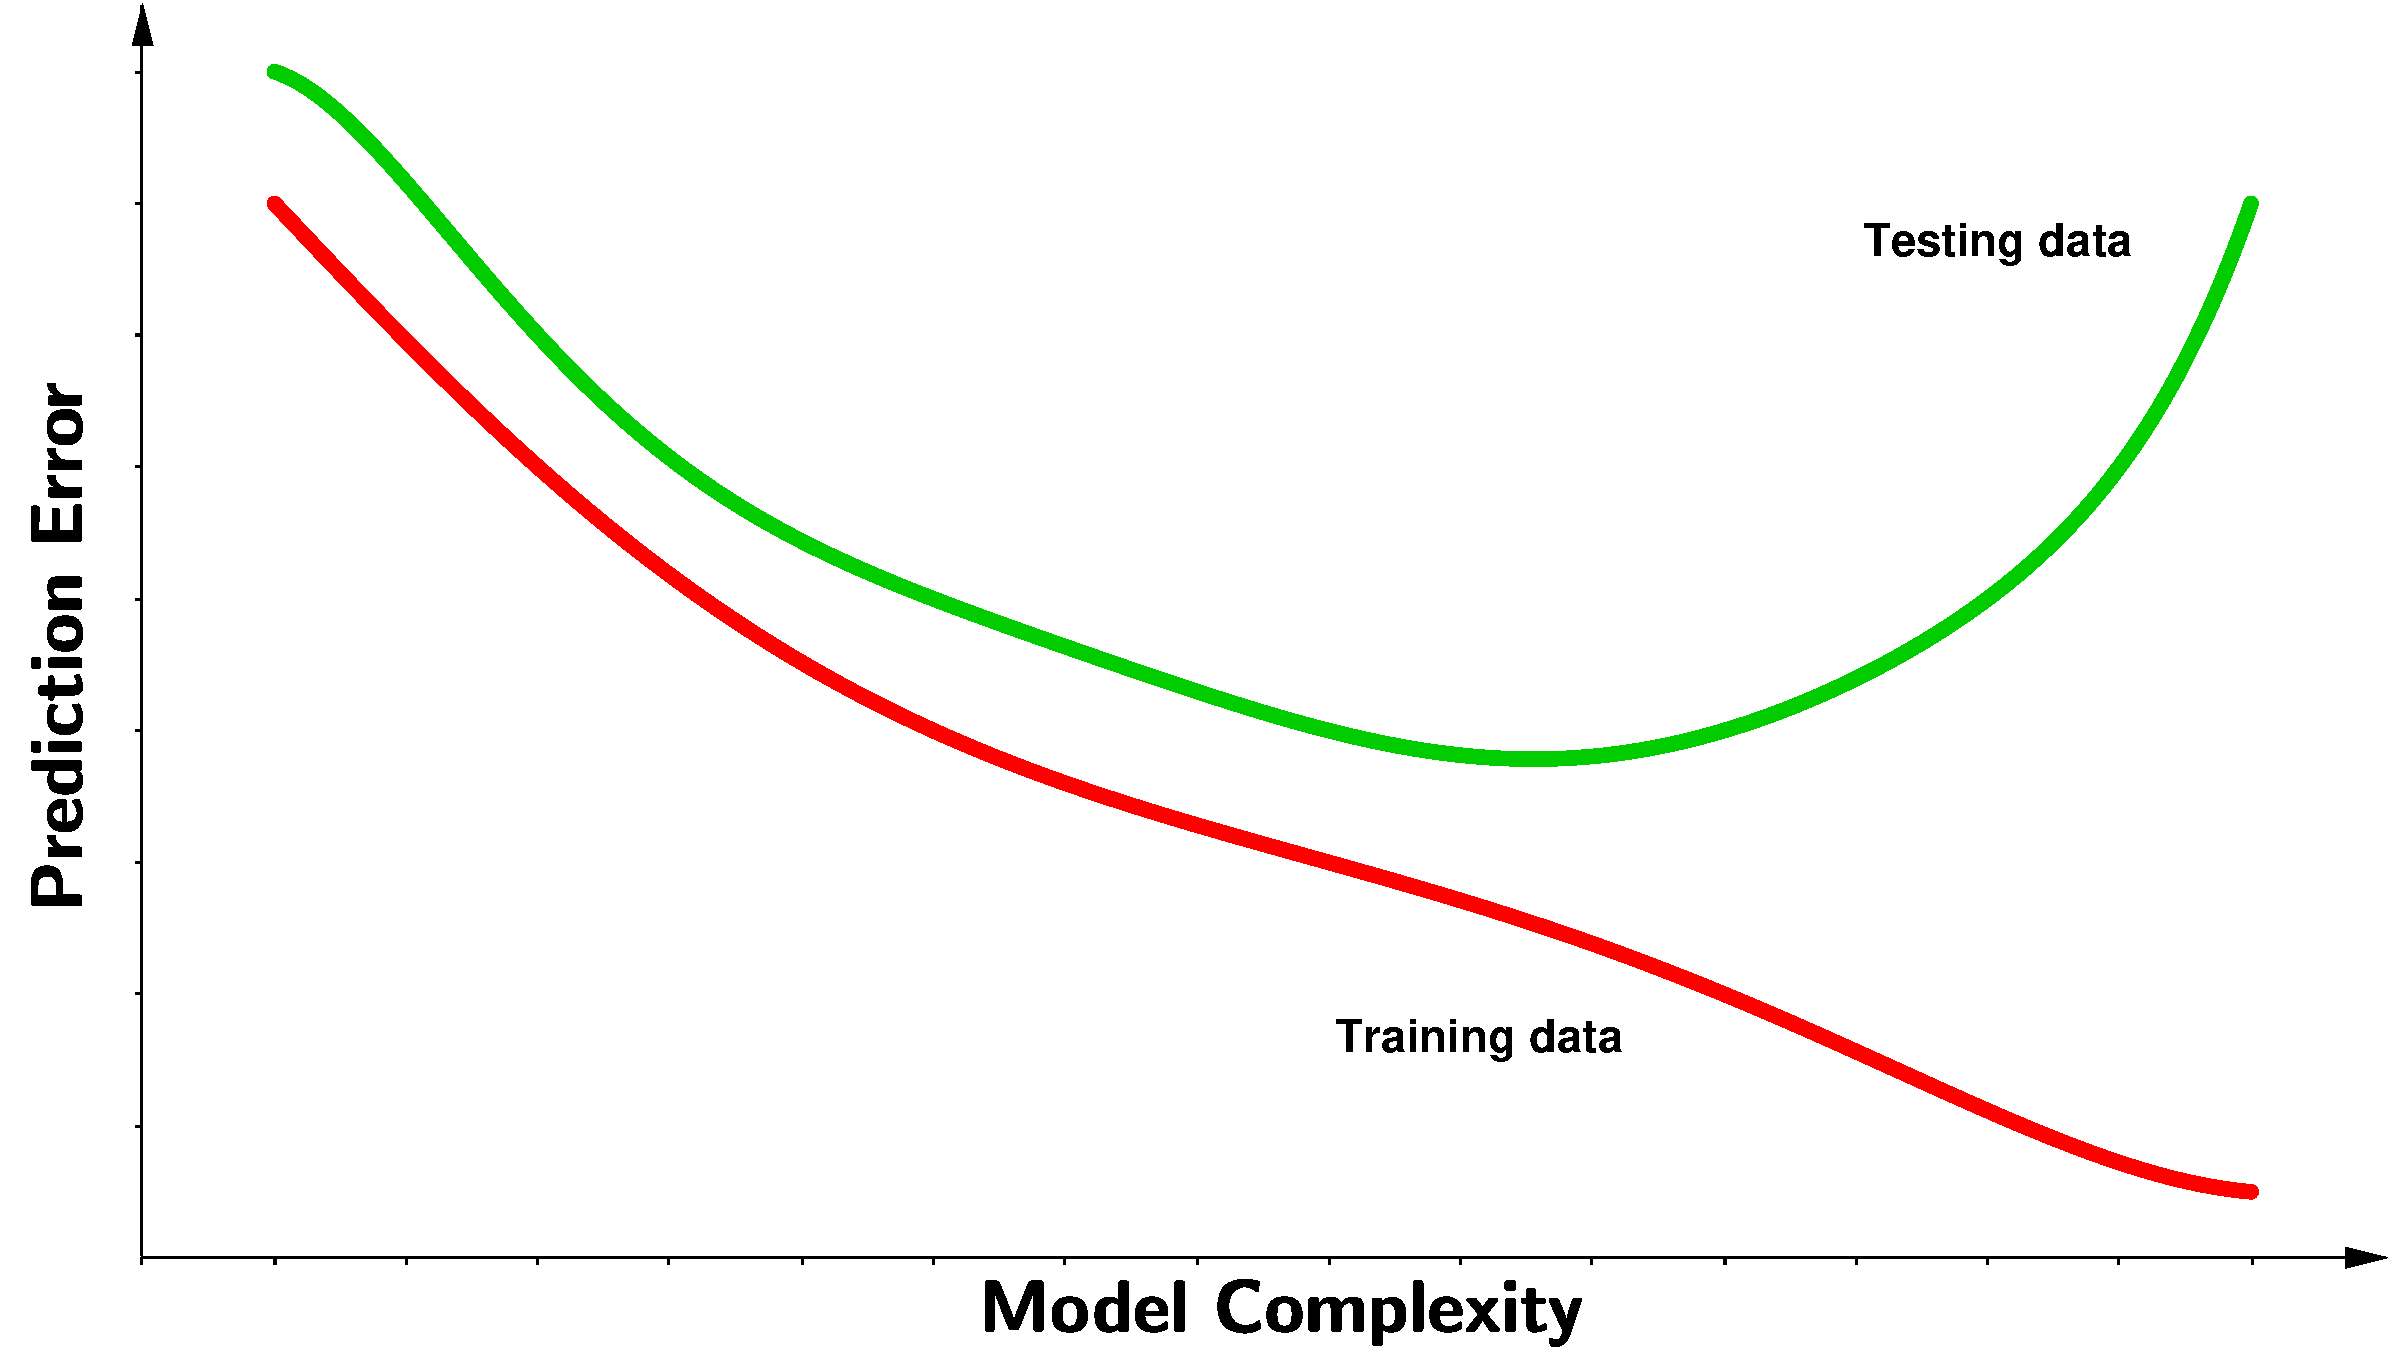
\includegraphics[width=16.0cm]{plots/Images/PE3.pdf}
	\caption{Evaluation of prediction error as a function of model complexity.}%
	\label{fig:Prediction_error}%
\end{figure}

\section{Cross-Validation}
The simplest and most widely used method for estimating prediction error of  the model $\hat{f}_{\boldsymbol{\theta}}$ is called \emph{cross-validation} (CV) \cite{statistics}. It is used for direct estimating of the expected extra-sample error
\begin{equation}
	\widehat{\mathrm{Err}} = \E\left[\mathcal{L}\left(y, \widehat{y}\right)\right],
\end{equation}
the measure how accurately is the model able to predict output values for previously unseen data - independent test sample. 


\subsection{K-Fold Cross-Validation}
In an ideal case, if we have sufficient number of data, we can set aside a test set and use
it to assess the performance of our prediction model. Since data are often
scarce, this is usually not possible. Very elegant solution to this problem is via K-fold cross-validation \cite{statistics}. It
uses part of the available data for fitting the model, and a different
part for testing. We split the data into $K$ roughly equal-sized parts, for
example, when $K = 5$, the scenario is shown in Figure \ref{fig:KFOLD}. 
\begin{figure}[h]
\begin{center}
\begin{tikzpicture}
\draw[step=2cm,gray,very thin] (0,0) grid (10,2); 
\draw (5,1) node{test};
\draw (1,1) node{train};
\draw (3,1) node{train};
\draw (7,1) node{train};
\draw (9,1) node{train};
\end{tikzpicture}
\end{center}
\caption{Splitting the data into $K=5$ roughly equal-sized parts.}
\label{fig:KFOLD}
\end{figure}

For the $j^{\mathrm{th}}$ part (third in Figure \ref{fig:KFOLD}), we train the model to the other $K-1$ parts
of the data, and calculate the prediction error of the fitted model when
predicting the $j^{\mathrm{th}}$ part of the data. We repeat this process for $j = \left\lbrace 1,2,\dots,K\right\rbrace$ and
combine the $K$ estimates of prediction error.\\
Let $\gamma : \left\lbrace 1,\dots,N\right\rbrace\rightarrow  \left\lbrace 1,\dots,K\right\rbrace$ be an indexing
function that indicates the partition to which observation $j$ is allocated by
the randomization. Symbol $\hat{f}_{\boldsymbol{\theta}}^{-j}\left(\boldsymbol{x}\right)$ denotes the fitted model, computed with
the $j^{\mathrm{th}}$th part of the data removed. Then the cross-validation estimate of
prediction error is defined by
\begin{equation}
\mathrm{CV}\left(\hat{f}_{\boldsymbol{\theta}}\right) = \frac{1}{N}\sum_{i = 1}^{N}\mathcal{L}\left(y_i , \hat{f}_{\boldsymbol{\theta}}^{-\gamma\left(i\right)}\left(\boldsymbol{x}_i\right)\right).
\end{equation}
Typical choices of $K$ are 5 or 10 and even case $K = N$ that is known as \emph{leave-one-out} cross--validation. Generally, there is not an universal way of choosing $K$, since it strongly depends on the available number of data. \\
The biggest problem of this method is a fact that it is computionally very expensive. For extremely complicated and complex models that are trained for hours or days, is cross--validation inconvenient approach of estimating the prediction error. 



\chapter{Discriminative vs. Generative Models}\label{discriminative_modelinmg}
\section{Overview}
Machine learning models can be classified into two main categories, discriminative and generative models. Simply put, a discriminative model makes predictions based on conditional probability $p\left(y|\bx\right)$ and is used for classification or regression problems. In other words, discriminative models distinguishes the decision boundary between the
classes.  It corresponds to learning parameters that maximize the conditional probability
distribution $p(y|\bx)$. On the contrary, a generative model revolves around the distribution of a data set to return a probability for a given example. Rather than
looking at classes and trying to find something to separate them, it focuses
only on the one class at the time and builds a model what that certain class looks like, then turns attention to the other class. To express it more formally, generative models learn parameters that maximize $p\left(\bx|y \right)$ and $p\left(y\right)$. Since
\begin{align}\label{eq:prob_decompostion}
p\left(\bx,y\right) = p\left(\bx|y\right)\cdot p\left(y\right),
\end{align}
with joint PDF it is possible to generate new $\left\lbrace\bx',y'\right\rbrace$ pairs. In some cases, the use of the second decomposition $p\left(\bx,y\right) = p\left(y|\bx\right)\cdot p\left(\bx\right)$ is also an option.  Note that in an unsupervised setting, the task is reduced to inferring only $p\left(\bx\right)$.
\begin{figure}[h]
	\centering
	\begin{minipage}{.5\textwidth}
		\centering
		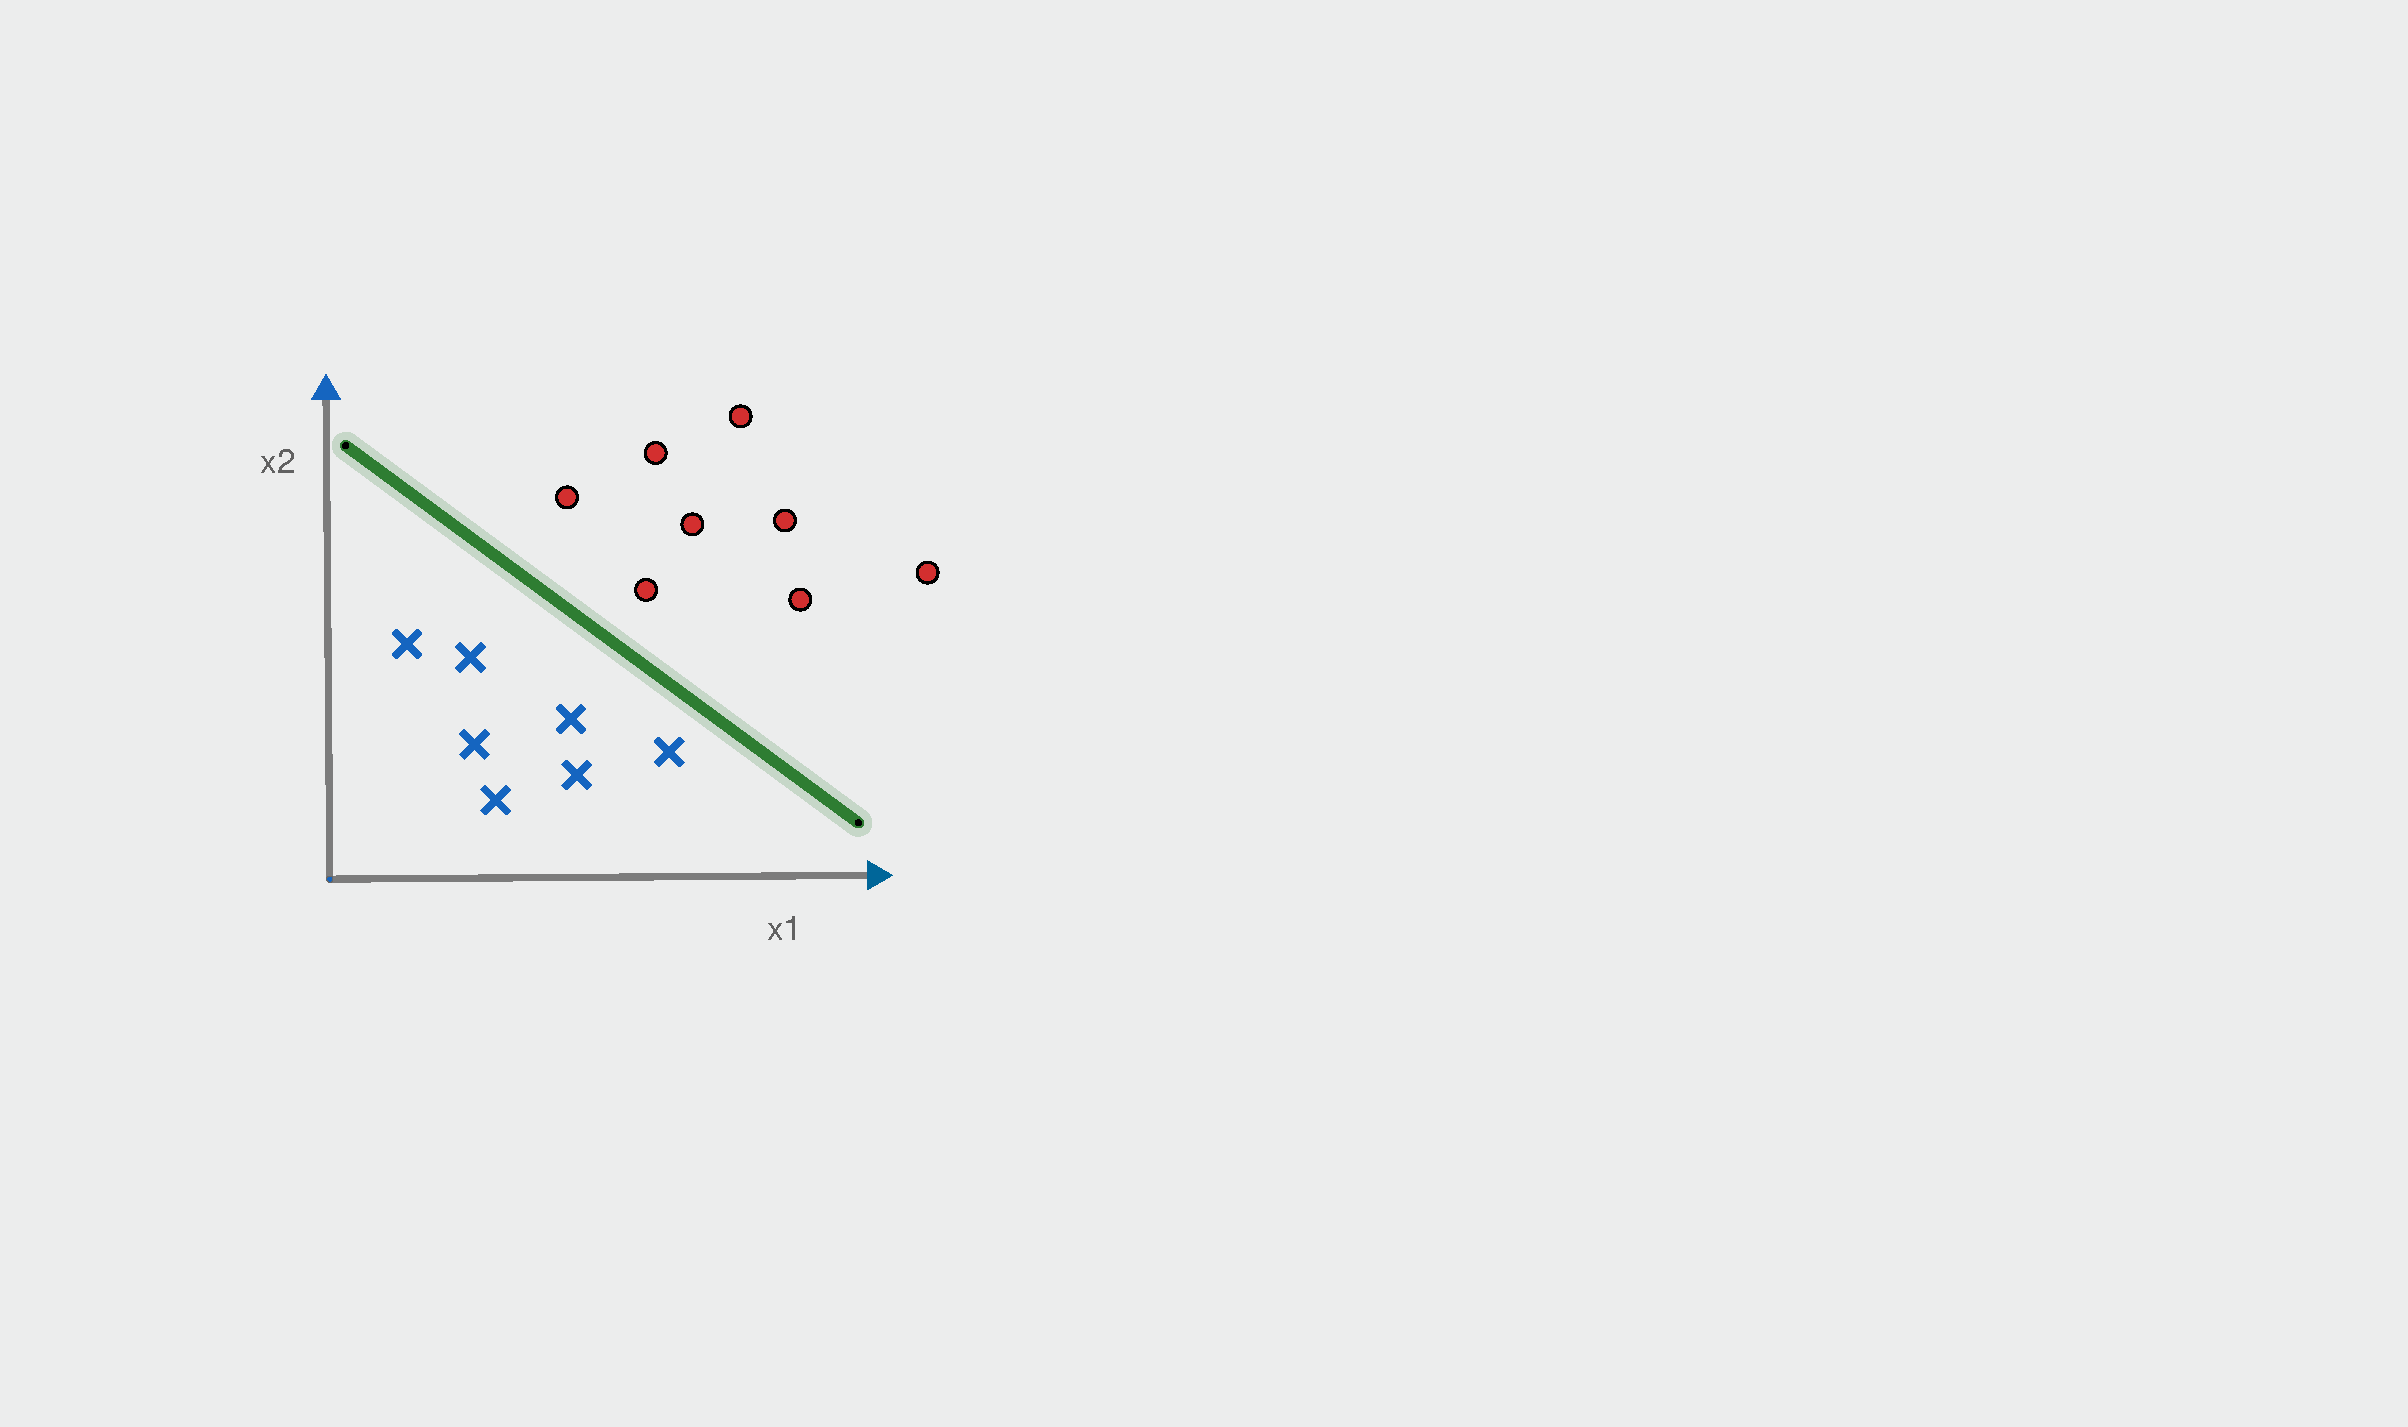
\includegraphics[trim = 4cm 8cm 24cm 6cm, clip = true, totalheight=0.26\textheight]{plots/Images/discriminative_model.pdf}
		\captionof{figure}{Discriminative approach. }
		\label{fig:test1}
	\end{minipage}%
	\begin{minipage}{.5\textwidth}
		\centering
		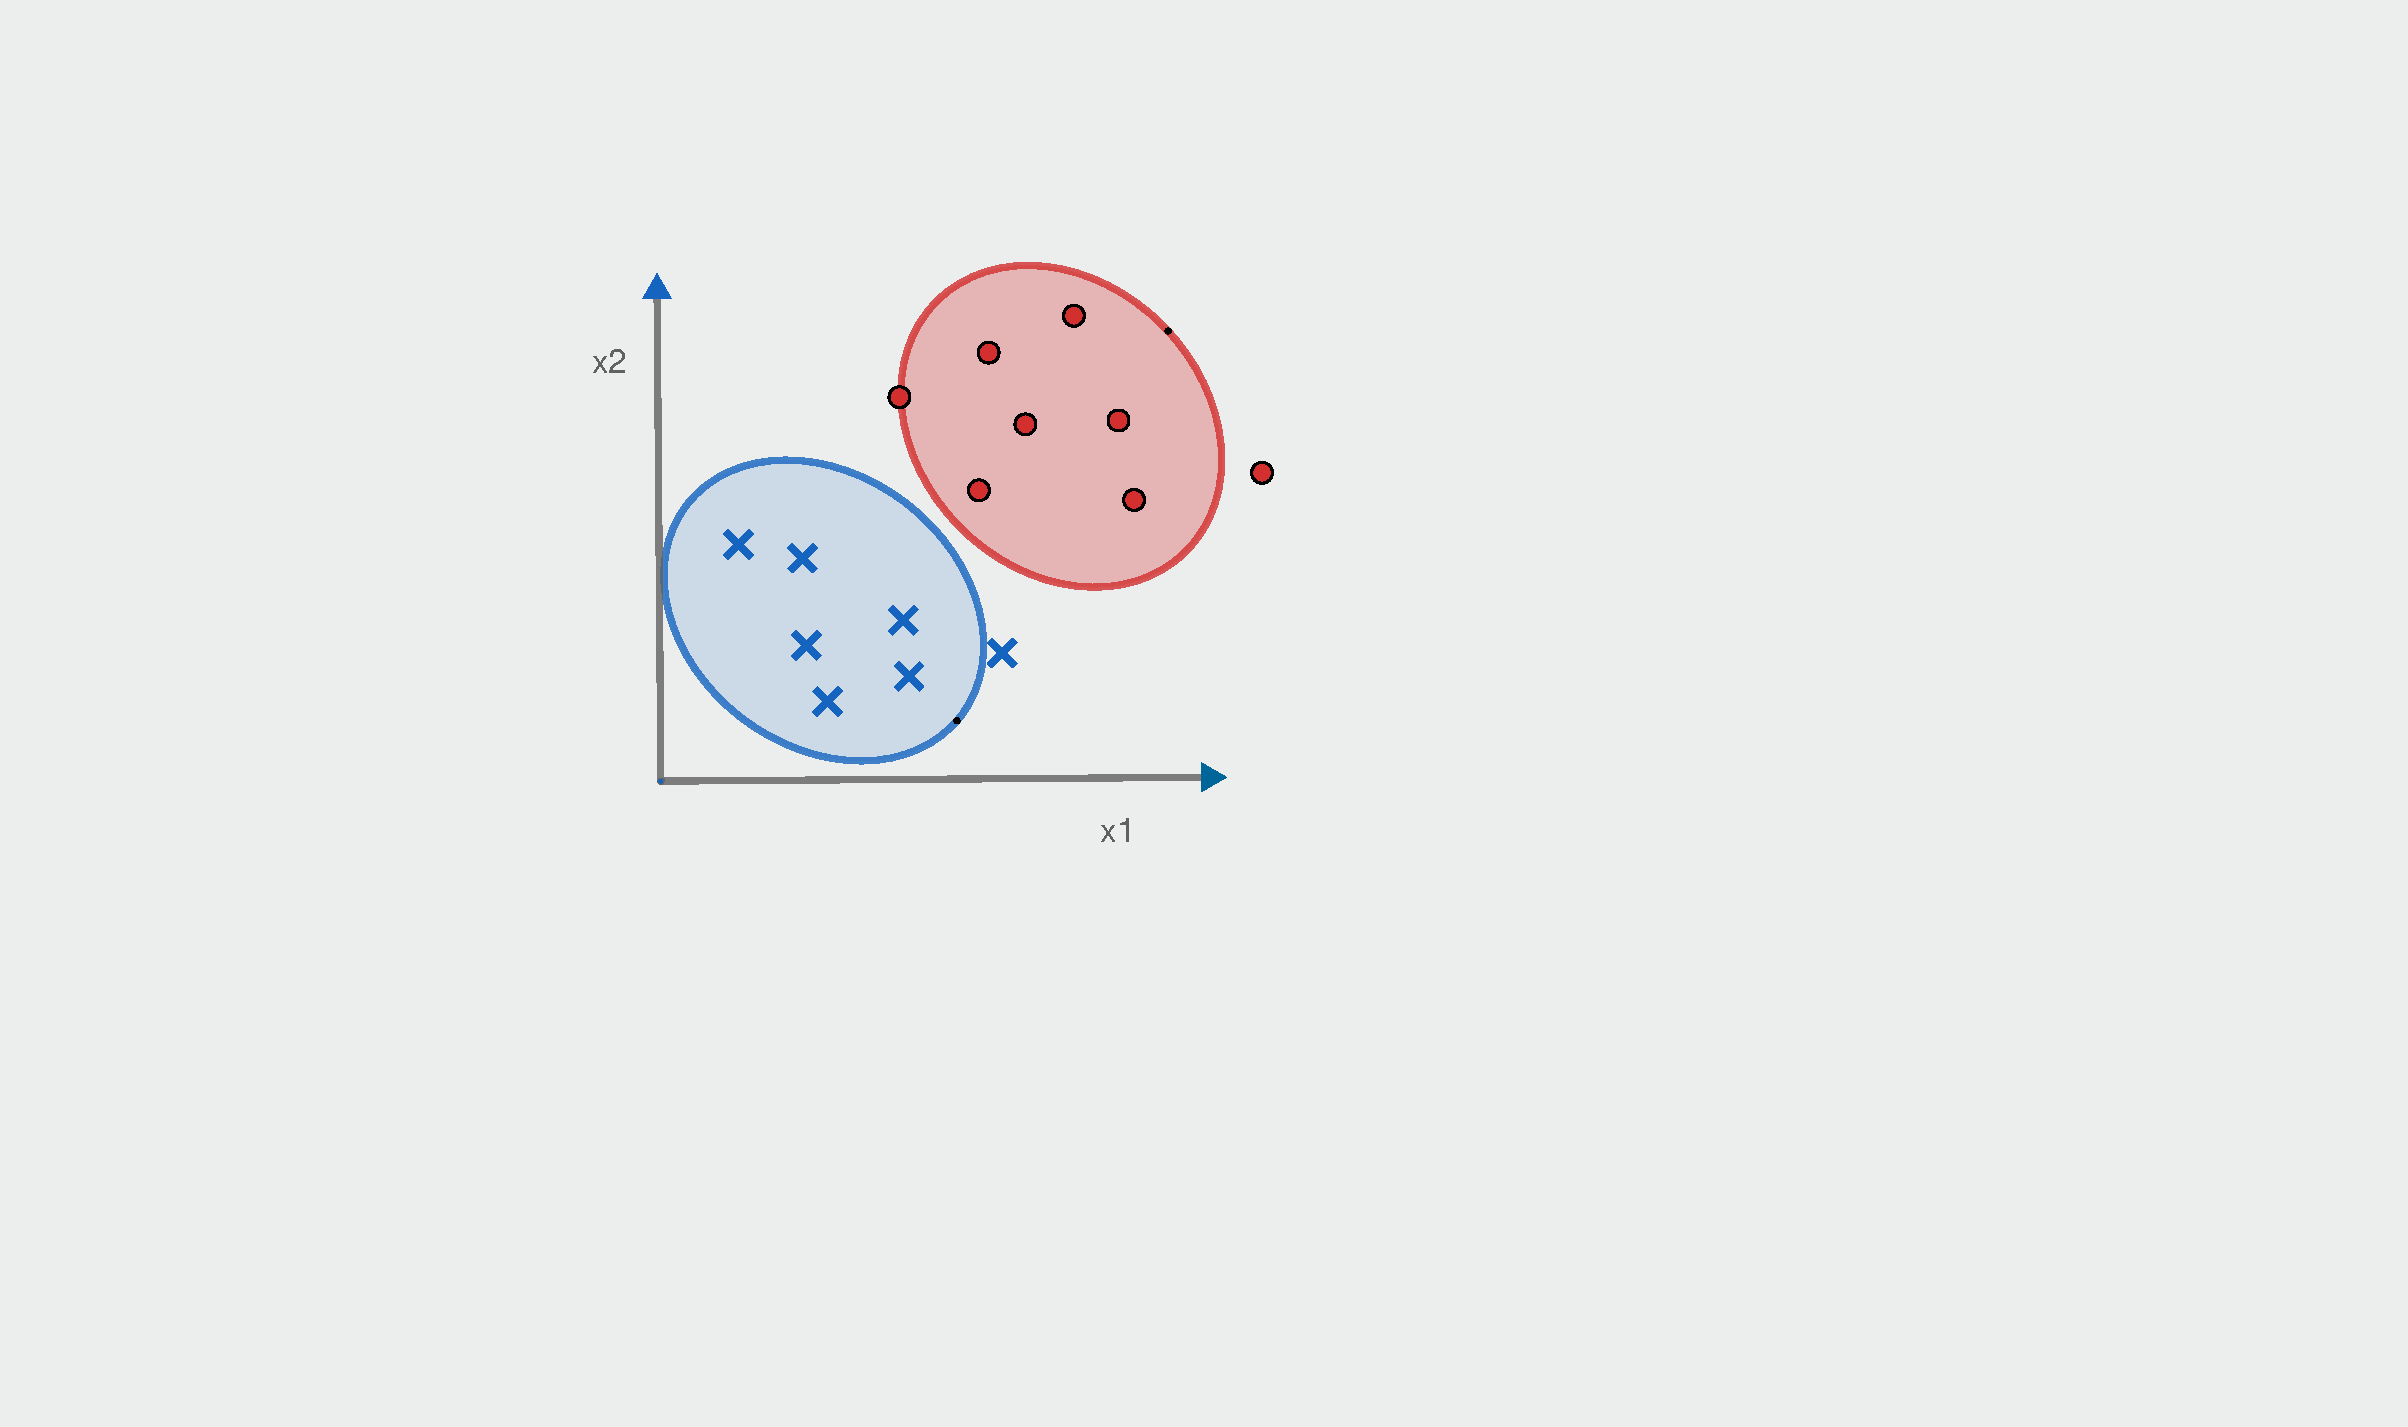
\includegraphics[trim =9.6cm 9.6cm 19cm 4cm, clip = true, totalheight=0.26\textheight]{plots/Images/generative_model.pdf}
		\captionof{figure}{Generative approach.}
		\label{fig:test2}
	\end{minipage}
%\caption{Discriminative and Generative approach.}
\end{figure}
\section{Discriminative Modeling}
In this section, we review the basics of discriminative modeling proposed in \cite{HDGEmain}. Given a data distribution through the probability density $p(\boldsymbol{x})$ and a label distribution with probability density $p(y|\boldsymbol{x})$ containing $C$ categories. In this thesis, we focus on classification problems, where the label $y$ is now a qualitative variable, taking on $C$ possible values and comes from a finite set $\pazocal{C}$.  A classification problem is typically solved using a parametric function $f_{\boldsymbol{\theta}}~:~\mathbb{R}^D~\to~\pazocal{C}$, where $\boldsymbol{\theta}$ denotes the parameters of the model. In practice, the function $f_{\boldsymbol{\theta}}$ is often used in the form of $\mathbb{R}^D \to  \mathbb{R}^C$. This function maps each data point $\boldsymbol{x} \in \mathbb{R}^D$ to $C$ real-valued numbers known as logits. It should be noted that $\mathbb{R}^C$ is allowed here due to the utilization of \emph{one-hot encoding}, which will be explained in Section \ref{OHE}. Logits are used to parameterize a categorical distribution through the function
\begin{equation}\label{softmax}
	q_{\boldsymbol{\theta}}\left(y|\boldsymbol{x}\right) = \frac{\exp\left({f_{\boldsymbol{\theta}}\left(\boldsymbol{x}\right)[y]}\right)}{\sum_{y\in\pazocal{C}}\exp\left({f_{\boldsymbol{\theta}}\left(\boldsymbol{x}\right)[y]}\right)},
\end{equation}
which is known as the Softmax. In other words, the data density $p\left(y\vert \bx\right)$ is modeled by a parameterized family of functions $\left\lbrace q_{\bt}\left(y\vert \bx\right) \vert \bt \in \Theta  \right\rbrace$ and thus $p\left(y\vert\bx\right)$ is assumed to belong to this family.   Note that the convention $f_{\boldsymbol{\theta}}\left(\boldsymbol{x}\right)[y]$ means the element $y^{\mathrm{th}}$ of $f_{\boldsymbol{\theta}}\left(\boldsymbol{x}\right)$. For learning $f_{\boldsymbol{\theta}}$ is usually minimized cross-entropy loss 
\begin{equation}\label{crossentropy}
     \mathrm{CE}\left(\bt\right)=-\mathbb{E}_{p_{\mathrm{data}}\left(y,\bx\right)}\left[\log q_{\boldsymbol{\theta}}\left(y|\boldsymbol{x}\right)\right] \approx -\frac{1}{N}\sum_{i=1}^N\log q_{\boldsymbol{\theta}}\left(y_i|\boldsymbol{x}_i\right).
\end{equation} 
The rationale for this objective comes from minimizing the Kullback-Leibler (KL) divergence with a target distribution $p(y| \boldsymbol{x})$ \cite{KL}. In general, the
KL divergence (or KL distance) from $p(y| \boldsymbol{x})$ to $q_{\boldsymbol{\theta}}\left(y|\boldsymbol{x}\right)$ is defined as
\begin{equation}\label{eq:KLdiv}
D_{\mathrm{KL}} \left(p(y| \boldsymbol{x}) || q_{\boldsymbol{\theta}}\left(y|\boldsymbol{x}\right) \right) = \int p(y| \boldsymbol{x})\log\frac{p(y| \boldsymbol{x})}{q_{\boldsymbol{\theta}}\left(y|\boldsymbol{x}\right)}\d{y} = \mathbb{E}_{p(y| \boldsymbol{x})} \left[\log\frac{p(y| \boldsymbol{x})}{q_{\boldsymbol{\theta}}\left(y|\boldsymbol{x}\right)} \right]
\end{equation}
and has the following properties:
\begin{enumerate}
\item $\KL{p(y| \boldsymbol{x})}{q_{\boldsymbol{\theta}}\left(y|\boldsymbol{x}\right)} \geq 0,$
\item $\KL{p(y| \boldsymbol{x})}{q_{\boldsymbol{\theta}}\left(y|\boldsymbol{x}\right)} = 0$ iff $p(y| \boldsymbol{x}) = q_{\boldsymbol{\theta}}\left(y|\boldsymbol{x}\right)$ almost everywhere,
\item $\KL{p(y| \boldsymbol{x})}{q_{\boldsymbol{\theta}}\left(y|\boldsymbol{x}\right)} \neq \KL{q_{\boldsymbol{\theta}}\left(y|\boldsymbol{x}\right)}{p(y| \boldsymbol{x})}$ and KL divergence does not obey the triangle inequality.
\end{enumerate}
The third property indicates that care is needed in the syntax describing KL divergence. We say that \eqref{eq:KLdiv} is from $p(y| \boldsymbol{x})$ to $q_{\boldsymbol{\theta}}\left(y|\boldsymbol{x}\right)$. Using the logarithmic property, \eqref{eq:KLdiv} can be further rewritten in the form 
\begin{equation}
	 \mathbb{E}_{p(y| \boldsymbol{x})} \left[\log\frac{p(y| \boldsymbol{x})}{q_{\boldsymbol{\theta}}\left(y|\boldsymbol{x}\right)} \right] = 
	 \mathbb{E}_{p(y| \boldsymbol{x})} \left[\log p(y| \boldsymbol{x}) \right] - \mathbb{E}_{p(y| \boldsymbol{x})} \left[\log q_{\boldsymbol{\theta}}\left(y|\boldsymbol{x}\right) \right],
	\end{equation}
where subscript $\boldsymbol{\theta}$ emphasizes that $q_{\boldsymbol{\theta}}\left(y|\boldsymbol{x}\right)$ is the approximative density we get to control. Note that
the first term does not depend on $\bt$ and therefore minimizing either CE or KL divergence is equivalent. Finally, by minimizing with respect to $\bt$ we obtain
\begin{equation}
\min_{\boldsymbol{\theta}} D_{\mathrm{KL}} \left(p(y| \boldsymbol{x}) \Vert q_{\boldsymbol{\theta}}\left(y|\boldsymbol{x}\right) \right) = \min_{\boldsymbol{\theta}} - \E_{p(y| \boldsymbol{x})}\left[ \log q_{\boldsymbol{\theta}}\left(y|\boldsymbol{x}\right)\right].
\end{equation}
For the sake of clarity, the expected value will be discussed. In practice, it is dealt with with discrete data, so the term $\E_{ p(y| \boldsymbol{x})}\left[\log q_{\boldsymbol{\theta}}\left(y|\boldsymbol{x}\right)\right]$ takes the form of
\begin{equation}
    \E_{p(y| \boldsymbol{x})}\left[\log q_{\boldsymbol{\theta}}\left(y|\boldsymbol{x}\right)\right] \approx \sum_{k=1}^C p(y_k| \boldsymbol{x})\log q_{\boldsymbol{\theta}}\left(y_k|\boldsymbol{x}\right).
\end{equation}
This part deserves further discussion for a few reasons:
\begin{itemize}
    \item Maximum likelihood estimation (MLE) of $\bt$ is equivalent to minimizing the KL distance.
    \item One may encounter the concepts of minimization or maximization of CE.
\end{itemize}
To address these reasons, it is necessary to briefly review the MLE. The MLE principle assumes that the most reasonable
values for $\bt$ are those for which the probability of the observed sample is
highest. Since $q_{\boldsymbol{\theta}}\left(y|\boldsymbol{x}\right)$ is model PDF, we have to follow the objective function
\begin{equation}
   \pazocal{L}\left(\bt^{}\right)= \sum_{i=1}^{N}\log q_{\boldsymbol{\theta}}\left(y_i|\boldsymbol{x}_i\right),
\end{equation}
which is up to the factor $-\frac{1}{N}$ same as \eqref{crossentropy}. Clearly, this changes only the value of $\pazocal{L}\left(\bt^{}\right)$, but not the location of the optima, so from an optimization perspective, the distinction is not important. However, the negative sign is obviously important since it is the difference between maximizing and minimizing.
Further optimization of $\pazocal{L}\left(\bt\right)$ gives the point estimate
\begin{align}
    \widehat{\bt}_{\mathrm{ML}} &= \argmax_{\bt} \sum_{i=1}^{N}\log q_{\boldsymbol{\theta}}\left(y_i|\boldsymbol{x}_i\right)\label{eq:argmax}\\ 
    &=\argmin_{\bt} -\sum_{i=1}^{N}\log q_{\boldsymbol{\theta}}\left(y_i|\boldsymbol{x}_i\right)\label{eq:argmin}.
\end{align}
It is more common to minimize a function than to maximize it in practice and therefore log--likelihood function is inverted by adding a negative sign to the front yielding a negative log--likelihood. 
\subsection{One--hot encoding}\label{OHE}
 Machine learning (ML) algorithms can misinterpret the numeric values of labels if there exists a hierarchy between them. One--hot encoding is a very common approach for dealing with this issue, in order to improve the algorithm performance. Each unique category value is transformed into a new column and these dummy variables are then filled with 0 or 1 (0 for FALSE and 1 for TRUE). For the sake of clarity, the transformation of a label encoding into a one--hot encoding is illustrated in the following table \ref{tab:OHE}. 
 
 However, this method has its own downsides. For example, it creates new variables and if there exist many unique category values, the models have to deal with a large number of predictors, leading to the so-called \emph{Big-p problem} \cite{Bigp}. Also, one--hot encoding causes multicolinearity between the individual variables, which may lead to reducing the model's accuracy. 
 \begin{table}[h]
 \centering
 	\begin{tabular}{|l|l|l|}
 		\hline
 		Food Name & Categorical \# & Calories \\ \hline
 		Pizza     & 1              & 266      \\ \hline
 		Hamburger & 2              & 295      \\ \hline
 		Caviar    & 3              & 264      \\ \hline
 	\end{tabular}
 	\quad $\Rightarrow$ \quad
	\begin{tabular}{|l|l|l|l|}
		\hline
		Pizza & Hamburger & Caviar & Calories \\ \hline
		1     & 0         & 0      & 266      \\ \hline
		0     & 1         & 0      & 295      \\ \hline
		0     & 0         & 1      & 264      \\ \hline
	\end{tabular}
	\caption{Transformation of a label encoding (left) to the one--hot encoding (right).}
	\label{tab:OHE}
 \end{table}
\section{Generative Modeling}

\subsection{Variational autoencoder}
The first generative modeling approach that will be discussed is the variational autoencoder (VAE). In this section, motivation will be addressed and individual mathematical aspects will be discussed in detail. 
\subsubsection{Problem scenario}
Assume that the data $\boldsymbol{X}=\left\lbrace x_i \right\rbrace^N_{i=1}$ are generated by some random process involving an unobserved continuous variable $\boldsymbol{z}$, which will be referenced as a latent variable or code. The objective is again to find the PDF of the given data in parametric form $p_{\bt}\left(\bx\right)$. One can choose an approximative distribution in the form of
\begin{equation}\label{eq:VAE_approxform}
p_{\bt}\left(\bx\right) = \int p_{\bt}\left(\bx,  \boldsymbol{z}\right)\d{\boldsymbol{z}} =\int p_{\bt}\left(\bx\vert \boldsymbol{z}\right)p_{\bt}\left(\boldsymbol{z}\right)\d{\boldsymbol{z}},
\end{equation}
But such an approximation is usually very expensive to compute or can even be intractable. Intractability of the $p_{\bt}\left(\bx\right)$ makes posterior PDF $p_{\bt}\left(\boldsymbol{z}\vert\bx\right)$ also intractable.

\subsubsection{Naive approach}
One of the simplest ways to solve this problem may seem to be to build a model depending on the latent variable $f_{\bt}\left(\boldsymbol{z}\right)$ and try to train its parameters. For simplicity, let $p\left(\boldsymbol{z} \right) = \pazocal{N}\left(\boldsymbol{0}, \mathbb{I}_P\right)$, where $P$ denotes the dimension of the latent space $\boldsymbol{z}$ and also let
\begin{equation}
\bx = f_{\bt}\left(\boldsymbol{z}\right) + \boldsymbol{\varepsilon}, \quad \boldsymbol{\varepsilon} \sim \pazocal{N}\left(\boldsymbol{0},\sigma^2\cdot\mathbb{I}_D \right)
\end{equation}
which actually gives 
\begin{equation}\label{eq:VAE_decoder}
p_{\bt}\left(\bx\vert\boldsymbol{z}\right) = \pazocal{N}\left(\boldsymbol{x};f_{\bt}\left(\boldsymbol{z}\right),\sigma^2\cdot\mathbb{I}_D \right).
\end{equation}
It may be noted that the subscript $D$ is the dimension of the data point $\bx$. The true PDF of the given data can be cleverly written using the empirical PDF, i.e., in the form of $p_{\mathrm{emp}}\left(\boldsymbol{x} \right)~=~\frac{1}{N}\sum_{i=1}^N\delta\left(\bx - \bx_i\right) $,
which can be exploited by finding the $\bt$ parameters by minimizing the $\KL{p_{\mathrm{emp}}\left(\boldsymbol{x} \right)}{p_{\bt}\left(\bx\right)}$. Since minimizing the KL distance is equivalent to ML estimation and using the approximative form \eqref{eq:VAE_approxform}, the following holds 
\begin{align}
    \widehat{\boldsymbol{\bt}} &= \argmin_{\boldsymbol{\bt}}- \sum_{i=1}^N\log p_{\boldsymbol{\bt}}\left(\boldsymbol{x}_i \right)\\
    &=  \argmin_{\boldsymbol{\bt}}- \sum_{i=1}^N \log \int \pazocal{N}\left(\boldsymbol{x}_i;f_{\bt}\left(\boldsymbol{z}\right),\sigma^2\cdot\mathbb{I}_D \right) \cdot \pazocal{N}\left(\boldsymbol{z};\boldsymbol{0}, \mathbb{I}_P\right) \d{\boldsymbol{z}}\\
    &= \argmin_{\boldsymbol{\bt}}- \sum_{i=1}^N \log \sum_{j=1}^{P}\exp\left(-\frac{1}{2\sigma^2}\left(\bx_i-f_{\bt}\left(\boldsymbol{z}_j\right)\right)^\top\left(\bx_i-f_{\bt}\left(\boldsymbol{z}_j\right)\right) \right).
\end{align}
Integration over $\boldsymbol{z}$ is represented by sampling. In iterations, for an incorrect value of $\bt$, all the generated samples may
be away from the samples of $\boldsymbol{x}$, and the gradient is poor.


\subsubsection{Variational Bayes approach}
\begin{figure}[h]
	\centering
	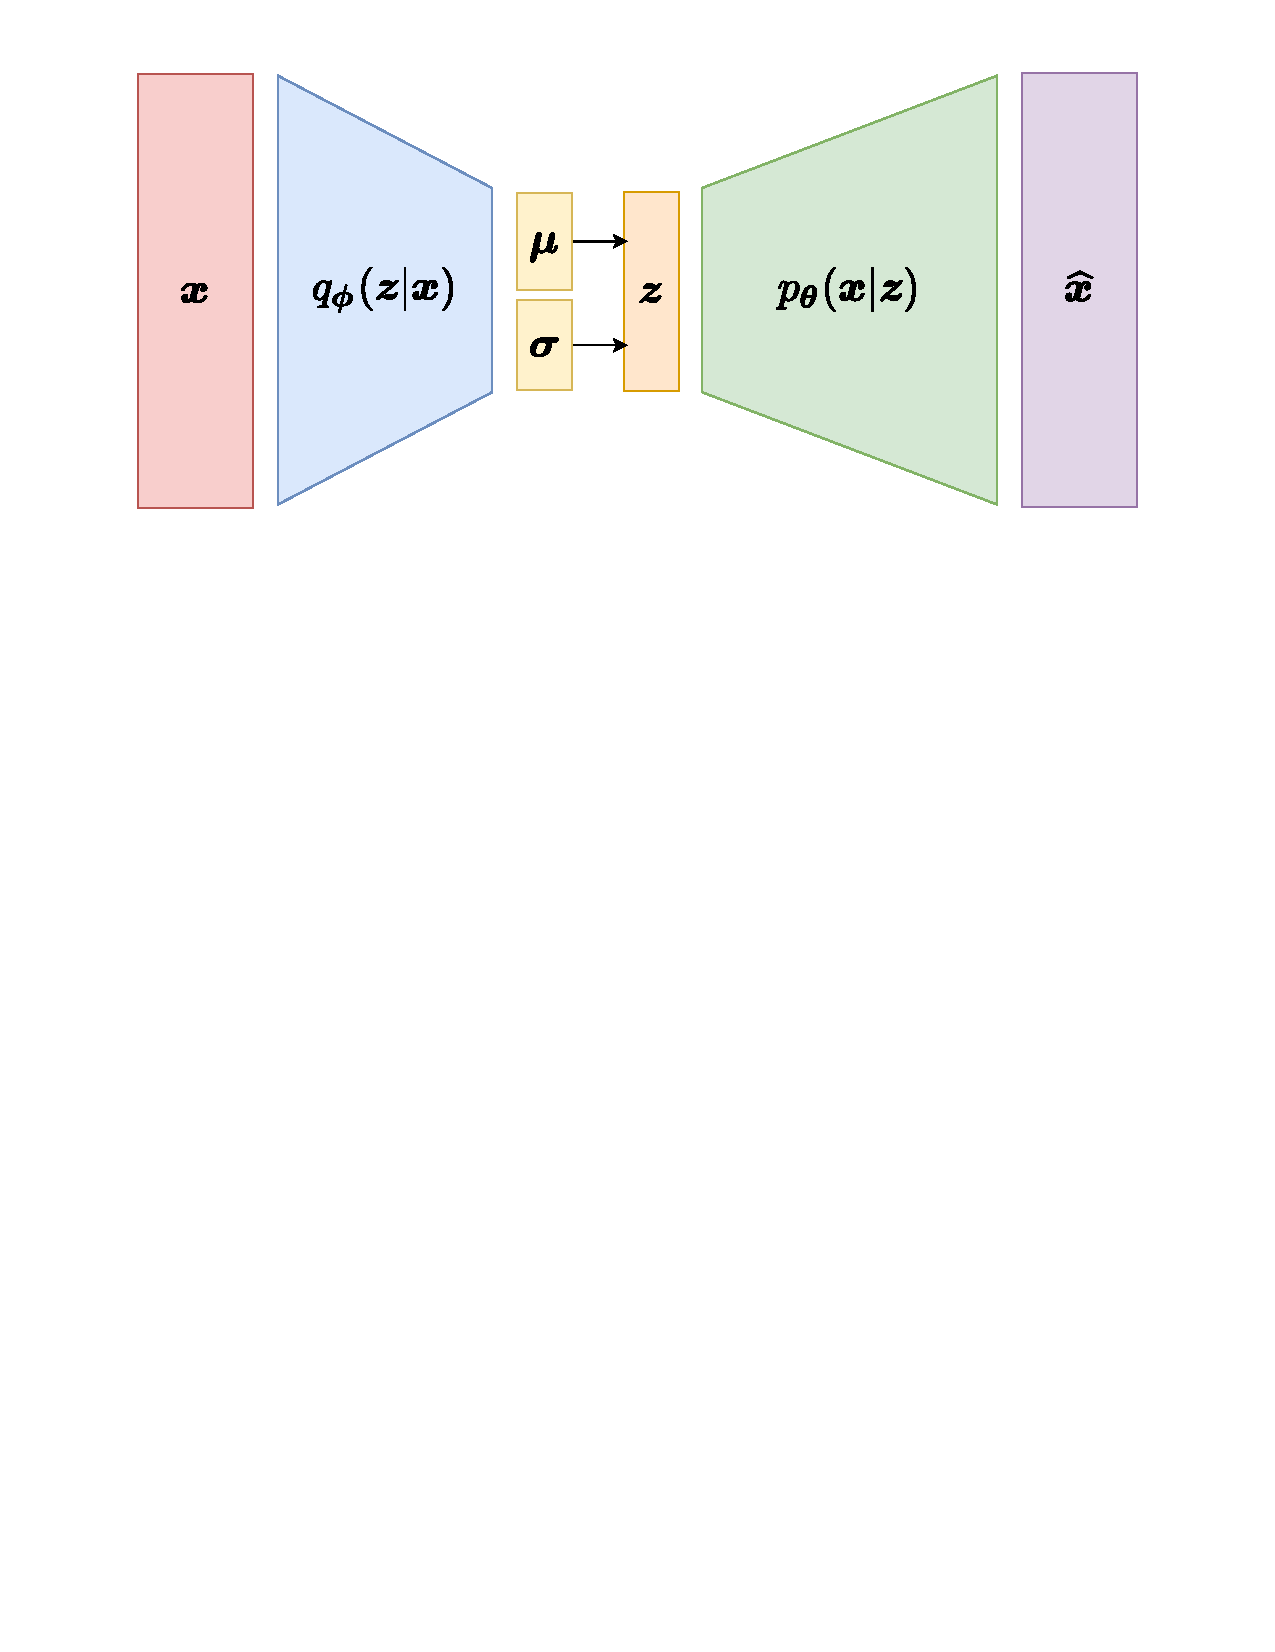
\includegraphics[width=\textwidth, trim={0 19cm 0 0cm}]{plots/Images/VAE_diagram.pdf}
	\caption{VAE diagram.}%
	\label{fig:VAE_architecture}%
\end{figure}

To solve this problem, it is necessary to introduce a further approximative posterior distribution $q_{\bphi}\left(\boldsymbol{z}\vert\bx\right) \approx p_{\bt}\left(\boldsymbol{z}\vert\bx\right)$ with parameters $\bphi$, preferably Gaussian. Standard terminology refers to the model $q_{\bphi}\left(\boldsymbol{z}\vert\bx\right)$ as a probabilistic \emph{encoder} and  $p_{\bt}\left(\bx\vert \boldsymbol{z}\right)$ is called a probabilistic \emph{decoder}. For VAE, the idea is to use the KL distance from $q_{\bphi}\left(\boldsymbol{z}\vert\bx\right)$ to $p_{\bt}\left(\boldsymbol{z}\vert \bx\right)$, which produces
\begin{equation}\label{eq:VAEloss}
\begin{split}
D_{\mathrm{KL}}\left(q_{\bphi}\left(\boldsymbol{z}\vert \bx \right) \Vert p_{\bt}\left(\boldsymbol{z}\vert \bx\right)\right) & = 
\int q_{\bphi}\left(\boldsymbol{z}\vert \bx \right) \log \frac{q_{\bphi}\left(\boldsymbol{z}\vert \bx \right)}{p_{\bt}\left(\boldsymbol{z}\vert \bx\right)} \d{\boldsymbol{z}} \\
& =  \int q_{\bphi}\left(\boldsymbol{z}\vert \bx \right) \log \frac{q_{\bphi}\left(\boldsymbol{z}\vert \bx \right)p_{\bt}\left(\bx\right)}{p_{\bt}\left(\bx \vert \boldsymbol{z}\right) p_{\bt}\left(\boldsymbol{z}\right)} \d{\boldsymbol{z}} \\
& = \log p_{\bt}\left(\boldsymbol{x}\right) +  \int q_{\bphi}\left(\boldsymbol{z}\vert \bx \right) \log \frac{q_{\bphi}\left(\boldsymbol{z}\vert \bx \right)}{p_{\bt}\left(\bx \vert \boldsymbol{z}\right)p_{\bt}\left(\boldsymbol{z}\right) } \d{\boldsymbol{z}} \\
& = \log p_{\bt}\left(\boldsymbol{x}\right) +  \mathbb{E}_{q_{\bphi}\left(\boldsymbol{z}\vert \bx \right)}\left[\log\frac{q_{\bphi}\left(\boldsymbol{z}\vert \bx \right)}{p_{\bt}\left(\boldsymbol{z}\right)} - \log p\left(\textbf{x}\vert \boldsymbol{z}\right)\right]\\
    & = \log p_{\bt}\left(\boldsymbol{x}\right) +\KL{q_{\bphi}\left(\boldsymbol{z}\vert \bx \right)}{p_{\bt}\left(\boldsymbol{z}\right)} -  \mathbb{E}_{q_{\bphi}\left(\boldsymbol{z}\vert \bx \right)}\left[\log p\left(\bx\vert \boldsymbol{z}\right)\right].
 \end{split}
\end{equation}
Using the last equality of \eqref{eq:VAEloss}, it is possible to rewrite the equation in its typical form
\begin{equation}
\log p_{\bt}\left(\bx\right) - D_{\mathrm{KL}}\left(q_{\bphi}\left(\boldsymbol{z}\vert \bx \right) \Vert p_{\bt}(\boldsymbol{z}\vert \bx)\right) = \underbrace{\mathbb{E}_{q_{\bphi}\left(\boldsymbol{z}\vert \bx \right)}\left[\log p_{\bt}(\bx\vert \boldsymbol{z}) \right] - D_{\mathrm{KL}}\left(q_{\bphi}\left(\boldsymbol{z}\vert\bx \right) \Vert p_{\bt}\left(\boldsymbol{z}\right)\right)}_{\text{= $L\left(\bt,\bphi; \bx\right)$}},
\end{equation}
where the right-hand side is called \emph{variational lower bound}. There is no uniformity in terminology, and thus one can also encounter the name evidence lower bound (ELBO). The first term on the right-hand side is known as reconstruction loss, and the second term is often called a regularization term. As a KL distance is always non-negative, it holds
\begin{equation}
    \log p_{\bt}\left(\bx\right) \geq L\left(\bt,\bphi; \bx\right).
\end{equation}
The objective is to maximize the log-likelihood $\log p_{\bt}\left(\bx\right)$ which is equivalent to minimizing the negative log-likelihood and that is what will be used here. At this point, we have a lower bound for one data point $\bx$, but we need to include all observations in the lower bound. The joint log-likelihood can be rewritten as a sum over the marginal log-likelihoods of individual observations $\log p_{\bt}\left(\bx_1,\bx_2,\dots,\bx_N\right)~=~\sum_{i=1}^N\log p_{\bt}\left(\bx_i\right)$ that completes all the building blocks needed to determine the optimization equation. This formulation provides one major advantage, which is that it is now possible to jointly optimize both the generative parameters $\bt$ and the variational parameters $\bphi$ as follows 
\begin{align}
   \widehat{\bt}, \widehat{\bphi} &= \argmin_{\bt,\bphi}-\sum_{i=1}^N\log p_{\bt}\left(\bx_i\right)\\
   &=\argmin_{\bt,\bphi}-\sum_{i=1}^N L\left(\bt,\bphi; \bx_i\right)\\
  &= \argmin_{\bt,\bphi}-\sum_{i=1}^N\mathbb{E}_{q_{\bphi}\left(\boldsymbol{z}\vert \bx_i \right)}\left[\log p_{\bt}(\bx_i\vert \boldsymbol{z}) \right] - D_{\mathrm{KL}}\left(q_{\bphi}\left(\boldsymbol{z}\vert\bx_i \right) \Vert p_{\bt}\left(\boldsymbol{z}\right)\right).\label{eq:VAEloss}
\end{align}
For a better understanding of the problem, a VAE diagram is shown in Figure \ref{fig:VAE_architecture}. Note that the latent space is usually much smaller than the input space, and for this reason, it is also sometimes called the bottleneck. 


\subsubsection{Reparameterization trick}
\begin{wrapfigure}{r}{0.45\textwidth}
  \begin{center}
    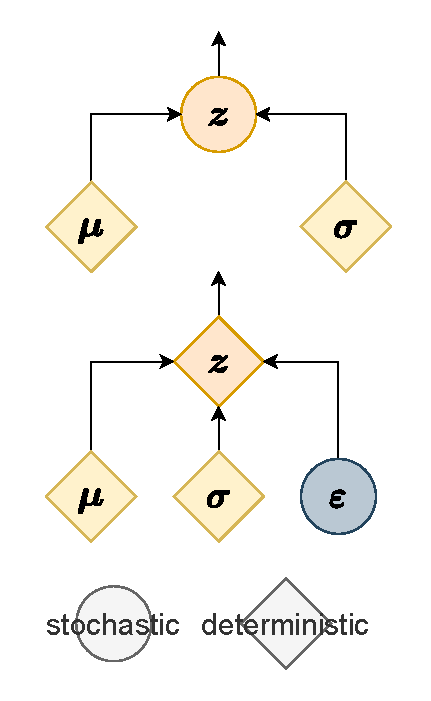
\includegraphics[trim={3cm 1.4cm 3cm 2.6cm}]{plots/Images/reparam_resized.pdf}
  \end{center}
  	\caption{Reparametrization trick.}%
	\label{fig:VAE_reparam}%
\end{wrapfigure}
The key success of VAE lies in the fact that \eqref{eq:VAEloss} can be efficiently computed using \emph{reparameterization trick}, where we express $\boldsymbol{z}$ as a deterministic variable
\begin{equation}\label{eq:reparam_general}
\boldsymbol{z} = g_{\bphi}\left(\boldsymbol{\varepsilon},\bx\right),
\end{equation}
 where $\boldsymbol{\varepsilon}$ stands for an auxiliary variable with independent marginal $p\left(\boldsymbol{\varepsilon}\right)$ and $g_{\bphi}\left(.\right)$ is a function parameterized by $\bphi$. 

A common explanation for this trick is that during the optimization the gradient cannot back--propagate through a random node. So, in the case of VAE, the reparameterization trick shifts the source of randomness to another variable different from $\boldsymbol{z}$ and allows differentiation with respect to $\boldsymbol{z}$. However, this explanation may not be sufficient and for this reason we will state a more formal justification. Consider taking the gradient with respect to $\bt$ of $\mathbb{E}_{p(\bz)}\left[\model{z} \right]$. It can be easily computed as
\begin{align}
    \nabla_{\bt}  \mathbb{E}_{p(\bz)}\left[\model{z} \right] &= \nabla_{\bt} \int p(\bz) \model{z} \d{\bz} \\
    &= \int p(\bz) \nabla_{\bt} \model{z} \d{\bz} \\
    &=  \mathbb{E}_{p(\bz)}\left[\nabla_{\bt}\model{z} \right].\label{eq:nonparametricexpectation}
\end{align}
The result is obvious; the gradient of the expectation is equal to the expectation of the gradient. However, the gradient of the expectation becomes much more interesting if the PDF $p_{\bt}(\bz)$ is also parameterized by $\bt$, resulting in 
\begin{align}
    \nabla_{\bt}  \mathbb{E}_{p_{\bt}(\bz)}\left[\model{z} \right] &= \nabla_{\bt} \int p_{\bt}(\bz) \model{z} \d{\bz} \\
    &= \int p_{\bt}(\bz) \nabla_{\bt} \model{z} \d{\bz} + \int  \model{z} \nabla_{\bt}p_{\bt}(\bz)\d{\bz} \\
    &=  \mathbb{E}_{p_{\bt}(\bz)}\left[\nabla_{\bt}\model{z} \right] + \int  \model{z} \nabla_{\bt}p_{\bt}(\bz)\d{\bz}. \label{eq:paramexpectation}
\end{align}
The second term of \eqref{eq:paramexpectation} is not guaranteed to be an expectation and this very fact indicates that backpropagation would not compute an estimate of $\nabla_{\bt}  \mathbb{E}_{p_{\bt}(\bz)}\left[\model{z} \right]$. That being the case, if we apply the reparameterization trick $\bz =g_{\bt}\left(\boldsymbol{\varepsilon},\bx\right)$ to this simple example, we get
\begin{equation}
\mathbb{E}_{p_{\bt}(\bz)}\left[\model{z} \right] = \mathbb{E}_{p(\boldsymbol{\varepsilon})}\left[f\left(g_{\bt}(\boldsymbol{\varepsilon}, \bx)\right) \right].
\end{equation}
At this point, it is possible to take the gradient $\nabla_{\bt} \mathbb{E}_{p(\boldsymbol{\varepsilon})}\left[f\left(g_{\bt}(\boldsymbol{\varepsilon}, \bx)\right) \right]$ analogously to that in \eqref{eq:nonparametricexpectation}. To be perfectly clear, the authors of [] proposed an easy exercise. Take the univariate Gaussian case $p(z|x) = \pazocal{N}\left(\mu, \sigma^2\right)$. In such a case, proper reparametrization takes the shape of
\begin{equation}\label{eq:VAE_reparam1D}
z = \mu + \sigma\varepsilon,
\end{equation}
where $\varepsilon\sim\pazocal{N}\left(0,1\right)$ and, therefore, the expectation
\begin{equation}
    \mathbb{E}_{\pazocal{N}\left(z;\mu, \sigma^2\right)}\left[f(z)\right] = \mathbb{E}_{\pazocal{N}\left(\varepsilon;0, 1\right)}\left[f(\mu + \sigma\varepsilon)\right] \approx \frac{1}{M}\sum_{j=1}^M f\left(\mu + \sigma\varepsilon_j\right).
\end{equation}
Note that this is nothing more than a transformation of a random variable. And this is exactly the problem with optimizing ELBO \eqref{eq:VAEloss}. We need to rewrite the expectation $\mathbb{E}_{q_{\bphi}\left(\boldsymbol{z}\vert\bx_i \right)}$ so that the Monte Carlo estimate of the expected value is differentiable with respect to $\boldsymbol{\phi}$.

\subsubsection{Variational autoencoder}
So far we have only dealt with VAE in general. In this section, we put everything together and specify the individual parts of the ELBO \eqref{eq:VAEloss}.
Let the probabilistic encoder be a multivariate Gaussian with a diagonal covariance matrix
\begin{equation}\label{eq:VAE_q}
q_{\bphi}\left(\boldsymbol{z}\vert \bx \right) = \pazocal{N}\left(\boldsymbol{z}; \boldsymbol{\mu},\boldsymbol{\sigma}^2\mathbb{I}_P  \right) 
\end{equation}
and let the probabilistic decoder takes the form depending on the type of given data and model.This is typically either multivariate Gaussian or Bernoulli. Finally, let the prior $p_{\bt}\left(\bz\right)$ be the centered izotropic multivariate Gaussian, i.e.
\begin{equation}
p_{\bt}\left(\boldsymbol{z} \right) = p\left(\boldsymbol{z} \right) = \pazocal{N}\left(\boldsymbol{z}; \boldsymbol{0},\mathbb{I}_P  \right),
\end{equation}
where the generative parameters $\bt$ are omitted, since the chosen prior distribution lacks parameters. When using \eqref{eq:VAE_q}, $\boldsymbol{\mu}$ and $\boldsymbol{\sigma}$ are non-linear functions of the data point $\bx$ and the variational parameters $\bphi$. This setting actually allows us to take the reparameterization trick in a form similar to that of Equation \eqref{eq:VAE_reparam1D}, which means that
\begin{equation}\label{eq:reparam_specific}
\boldsymbol{z}_{i,j} = \boldsymbol{\mu}_i + \boldsymbol{\sigma}_i\odot\boldsymbol{\varepsilon}_j ,
\end{equation}
where the symbol $\odot$ denotes the Hadamard product, i.e., the element-wise product and the auxiliary variable $\boldsymbol{\varepsilon} \sim \pazocal{N}\left(\boldsymbol{0},\mathbb{I} \right)$.
Another important fact is that the KL distance from a Gaussian distribution to a Gaussian distribution has an analytical solution, so $\KL{q_{\bphi}\left(\bz\vert \bx \right)}{p_{\bt}\left(\bz\right)}$ can be expressed in closed form:
\begin{equation}
\begin{split}
 \KL{q_{\bphi}\left(\bz\vert \bx \right)}{p_{\bt}\left(\bz\right)} & = \KL{\pazocal{N}\left(\boldsymbol{z}; \boldsymbol{\mu},\boldsymbol{\sigma}^2\mathbb{I}_P  \right) }{\pazocal{N}\left(\boldsymbol{z}; \boldsymbol{0},\mathbb{I}_P  \right)}\\ & =\frac{1}{2}\sum_{j=1}^P\left(1 + \log\sigma^2_j -\mu_j^2 -\sigma_j^2 \right).
\end{split}
\end{equation}
Now all that is left is to plug everything into equation \eqref{eq:VAEloss}, which leads to the final form
\begin{align}\label{řešení_VAE}
 \widehat{\bt}, \widehat{\bphi} & = \argmin_{\bt,\bphi}-\sum_{i=1}^N\mathbb{E}_{q_{\bphi}\left(\boldsymbol{z}\vert \bx_i \right)}\left[\log p_{\bt}(\bx_i\vert \boldsymbol{z}) \right] - D_{\mathrm{KL}}\left(q_{\bphi}\left(\boldsymbol{z}\vert\bx_i \right) \Vert p_{\bt}\left(\boldsymbol{z}\right)\right) \\
 & = \argmin_{\bt, \bphi}-\sum_{i = 1}^N\left(\frac{1}{P}\sum_{j = 1}^P \log p_{\bt}\left(\bx_i\vert \bz_{i,j}\right) +   \frac{1}{2}\sum_{j=1}^P\left(1 + \log\sigma^2_{i,j} -\mu_{i,j}^2 -\sigma_{i,j}^2 \right)\right).
\end{align}



\subsection{Noise--Contrastive Estimation}
Suppose one has to estimate a model that is specified by an non-normalized probability density function $q^0_{\bt}\left(\boldsymbol{x}\right)$. In such a case, one can utilize noise--contrastive estimation (NCE). The first step is to introduce another parameter $c$ among the estimated parameters $\bt$. For clarity, the symbol $\bt^\star=\left\lbrace\bt^{},c^{}_{}\right\rbrace$ is introduced for the set of estimated parameters, including
$c$. Using this notation, we can write the following equality
\begin{align}
    \log q_{\bt^\star}\left(\boldsymbol{x}\right) = \log q_{\bt^\star}^0\left(\boldsymbol{x}\right) + c,
    \end{align}
which means that the newly introduced parameter $c$ is an estimate of the negative logarithm of
the normalization constant $Z\left(\bt\right)$ \eqref{eq:partitionfunction}.
As the name suggests, we use noise to estimate. By our convention, let $\boldsymbol{X} = \left\lbrace\bx_1,\bx_2,\dots,\bx_N\right\rbrace$
be the observations and $\boldsymbol{\Xi} = \left\lbrace\boldsymbol{\varepsilon}_1,\boldsymbol{\varepsilon}_2,\dots,\boldsymbol{\varepsilon}_N\right\rbrace$ be the artificially generated noise data with known distribution $\psi\left(\boldsymbol{\varepsilon}\right)$. The estimate $\widehat{\bt^\star}$ is then defined as
\begin{align}
    \widehat{\bt^\star} &= \argmax_{\bt^\star} \pazocal{L}^{\mathrm{NC}}\left(\bt^\star\right)\\
   &= \argmax_{\bt^\star} \frac{1}{2N}\sum_{i=1}^N \log S_{\bt^\star}\left(\bx_i\right) + \log\left(1-S_{\bt^\star}\left(\boldsymbol{\varepsilon}_i\right) \right)\label{NCEloss1}\\
   &= \argmin_{\bt^\star} -\frac{1}{2N}\sum_{i=1}^N \log S_{\bt^\star}\left(\bx_i\right) + \log\left(1-S_{\bt^\star}\left(\boldsymbol{\varepsilon}_i\right) \right)\label{NCEloss2}
\end{align}
where $S_{\bt^\star}$ stands for a logistic function,
\begin{align}
S_{\bt^\star}\left(\bx\right) = \frac{1}{1 + \exp\left(-G_{\bt^\star}\left(\bx\right) \right)}
\end{align}
and finally, the function $G_{\bt^\star}$ represents the difference of the log-likelihoods of $q_{\bt^\star}$ and $\psi$, hence 
\begin{align}\label{eq:NCE_G}
    G_{\bt^\star}\left(\bx\right) = \log q_{\bt^\star}\left(\bx \right) - \log\psi\left(\bx \right).
\end{align}
It may be noted that equation \eqref{NCEloss1} also appears in SL tasks and is called binary
CE loss. It is actually a special case of CE itself. Thus, it is used for the classification of two classes. This gives an intuitive insight into how noise--contrastive estimation
really works. When data and noise are compared, the model is learned, so this method can be called
learning by comparison. To make the connection with SL more explicit, denote $U = \left\lbrace\boldsymbol{u}_1, \boldsymbol{u}_2,\dots,\boldsymbol{u}_{2N} \right\rbrace$ the union of two sets $\boldsymbol{X}$ and $\boldsymbol{\Xi}$. Then each data point $\boldsymbol{u}_i$ is assigned a binary class label $y_i$, where $y_i = 1$ if $\boldsymbol{u}_i \in \boldsymbol{X}$ and $y_i = 0$ if $\boldsymbol{u}_i \in \boldsymbol{\Xi}$. The aim is to estimate the posterior probabilities of the classes given the data $\boldsymbol{u}_i$. To do this, one needs the class--conditional PDFs that are given by
\begin{equation}
    p\left(\boldsymbol{u}\vert y =1 \right) =  q_{\bt^\star}\left(\boldsymbol{u} \right) \qquad p\left(\boldsymbol{u}\vert y =0 \right) =  \psi\left(\boldsymbol{u} \right).
\end{equation}
Class labels are equally likely, so that $\mathrm{Pr}\left(y = 1\right) =\mathrm{Pr}\left(y = 0\right)=\frac{1}{2}$ and the posteriors are determined as follows
\begin{align}
    \mathrm{Pr}\left( y=1 \vert\boldsymbol{u} \right) &= \frac{q_{\bt^\star}\left(\boldsymbol{u} \right)}{q_{\bt^\star}\left(\boldsymbol{u} \right) + \psi\left(\boldsymbol{u} \right)} = S_{\bt^\star}\left(\boldsymbol{u}\right),\\
    \mathrm{Pr}\left( y=0\vert \boldsymbol{u} \right) &= 1 - S_{\bt^\star}\left(\boldsymbol{u}\right).
\end{align}
The class labels $y_i$ are Bernoulli--distributed so that
for the log--likelihood of Bernoulli we get
\begin{align}
    \pazocal{L}^{\mathrm{NC}}\left(\bt\right) &= \sum_{i=1}^{2N} y_i\log \mathrm{Pr}\left( y=1 \vert\boldsymbol{u}_i \right) + \left(1-y_i\right)\log \mathrm{Pr}\left( y=0 \vert\boldsymbol{u}_i \right) \\
    &= \sum_{i=1}^{N}\log S_{\bt^\star}\left(\boldsymbol{x}_i\right) +\log \left(1 - S_{\bt^\star}\left(\boldsymbol{\epsilon}_i\right)\right),
\end{align}
which is the equation (up to extrinsic factor $\frac{1}{2N}$) that is optimized in \eqref{NCEloss1} or \eqref{NCEloss2}.
\subsubsection{Choice of the contrastive noise PDF}
The noise distribution $\psi\left(\boldsymbol{\varepsilon}\right)$ can be considered as a design parameter. But this choice is not completely arbitrary, because in practice the noise distribution should meet certain conditions. These are:
\begin{enumerate}
    \item It is easy to sample from, because NCE approach relies on artificially generated noise data $\boldsymbol{\varepsilon}_1,\boldsymbol{\varepsilon}_2,\dots,\boldsymbol{\varepsilon}_N$. 
    \item In order to smoothly evaluate \eqref{eq:NCE_G}, closed form for $\log\psi\left(. \right)$ is requisite.
    \item It leads to a small mean squared error $\mathbb{E}\left[\left(\widehat{\bt^\star} - \bt^\star\right)^2\right]$.
\end{enumerate}
The authors of [] suggest using a Gaussian or uniform distribution, eventually a Gaussian mixture. 
\begin{example}[One--dimensional Gaussian distribution]
\begin{figure}[h]
	\centering
	\subfloat[Loss function minimizing.]
	{{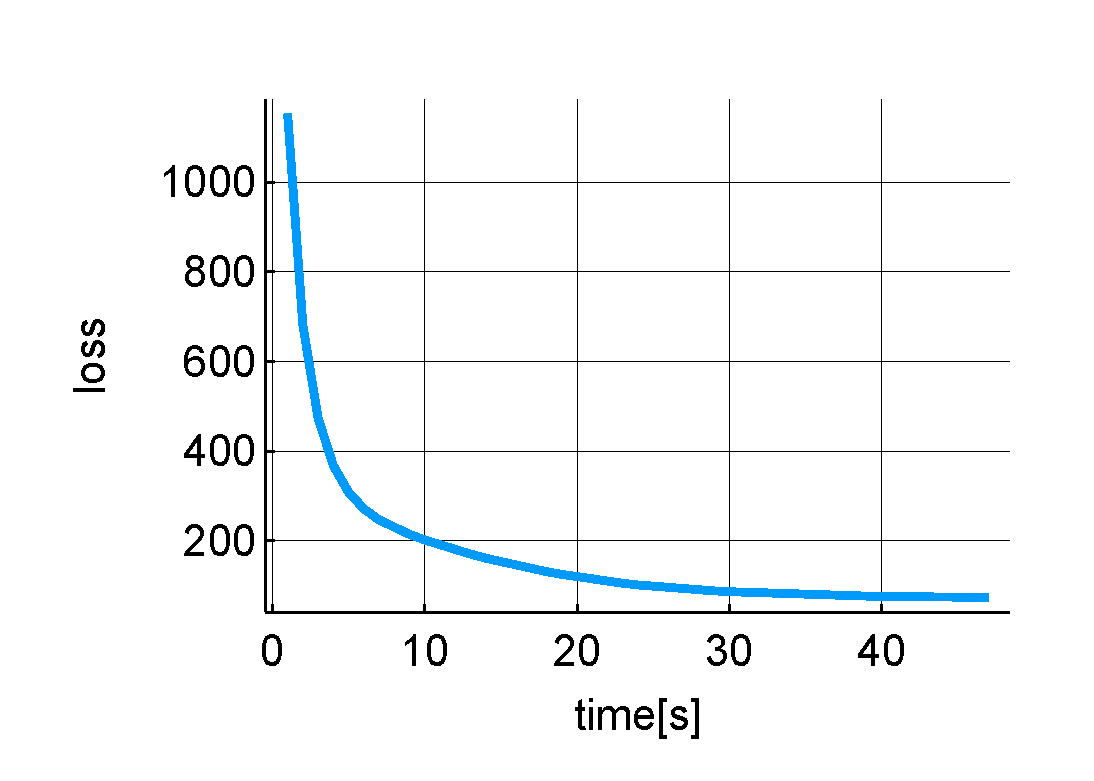
\includegraphics[width=8.0cm]{plots/Images/NCE_loss.pdf} }}%
	\subfloat[Comparison of true (blue) and estimated (red) PDF.]
	{{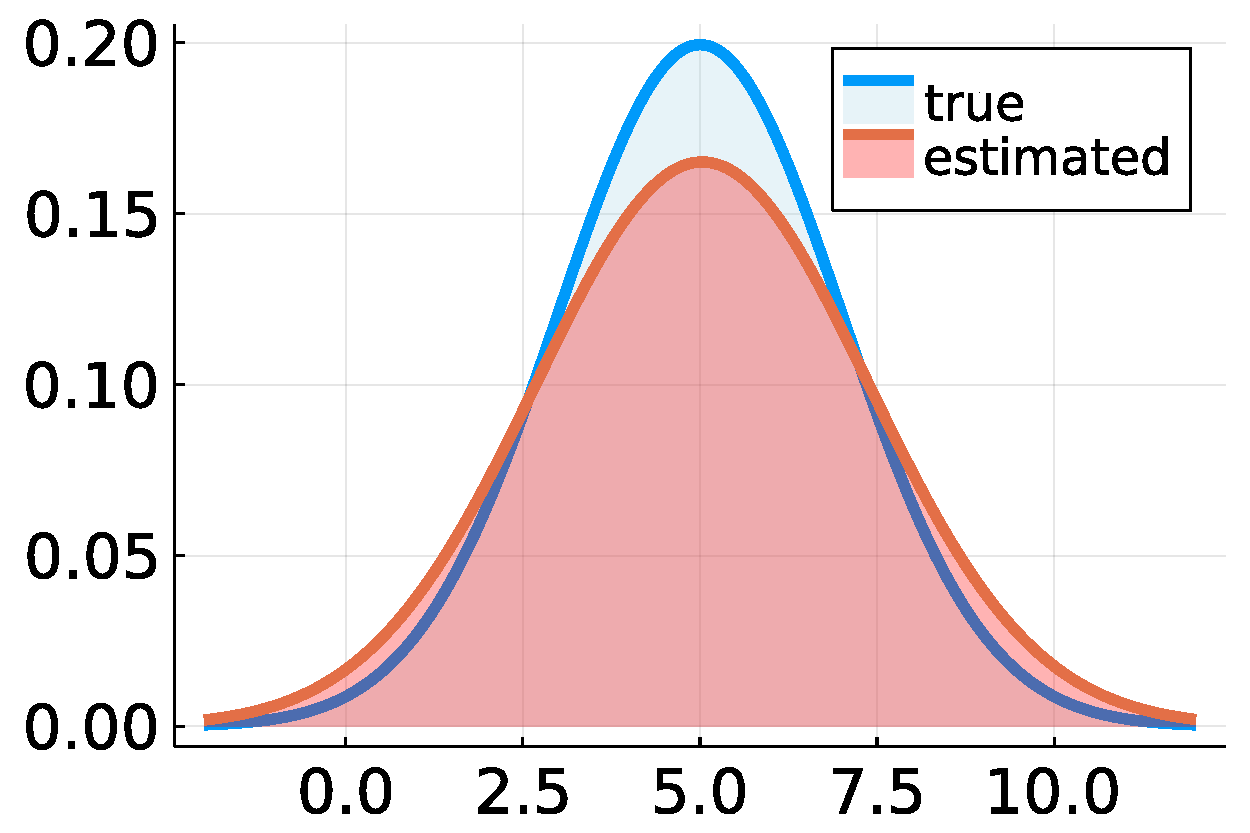
\includegraphics[width=8.0cm]{plots/Images/NCE_reselts2.pdf} }}%
	\caption{Results of the NCE experiment for one--dimensional Gaussian case.}%
	\label{ex:NCE_1}%
\end{figure}
\end{example}
To test this approach, we performed a simple experiment. There are a total of $N = 100$ i.i.d. and one-dimensional observations $x_1,x_2,\dots,x_N$ from an unknown distribution that is assumed to be non--normalized and Gaussian. Therefore, it is of the form
\begin{align}\label{eq:NCE_datadist1}
    q_{\bt^\star}\left(x\right) = \exp\left(-\frac{1}{2}\cdot\frac{\left(x-\mu\right)^2}{\sigma^2} + c \right),
\end{align} 
where $\bt^\star = \left\lbrace \mu, \sigma^2, c \right\rbrace$. Next, we artificially generate noise data $e_1,e_2,\dots,e_N$, which is again easier to do using a Gaussian distribution. This means that it can be chosen, for example,
\begin{align}\label{eq:NCE_noisedist1}
    \psi\left(e\right) = \frac{1}{\sqrt{2\pi 10}}\exp\left(-\frac{1}{2}\cdot\frac{e^2}{10} \right).
\end{align}
We choose the noise PDF intentionally so widely spread from its mean value because these two PDFs, i.e. \eqref{eq:NCE_datadist1} and \eqref{eq:NCE_noisedist1}, should at least partially overlap. At this point, we have all the components available and it is possible to construct a function $-\pazocal{L}^{\mathrm{NC}}\left(\bt^\star\right)$ that is minimized by using the ADAM optimization algorithm []. The following figure shows the training process and the comparison between
the estimated distribution and the true one. As can be seen in Figure \ref{ex:NCE_1}, this approach works quite well and for more observations, the results would be even better. In addition, the minimization of $-\pazocal{L}^{\mathrm{NC}}\left(\bt^\star\right)$ is very fast.


\begin{example}[Two--dimensional Gaussian distribution]
\begin{figure}[h]
	\centering
	\subfloat[Loss function minimizing.]
	{{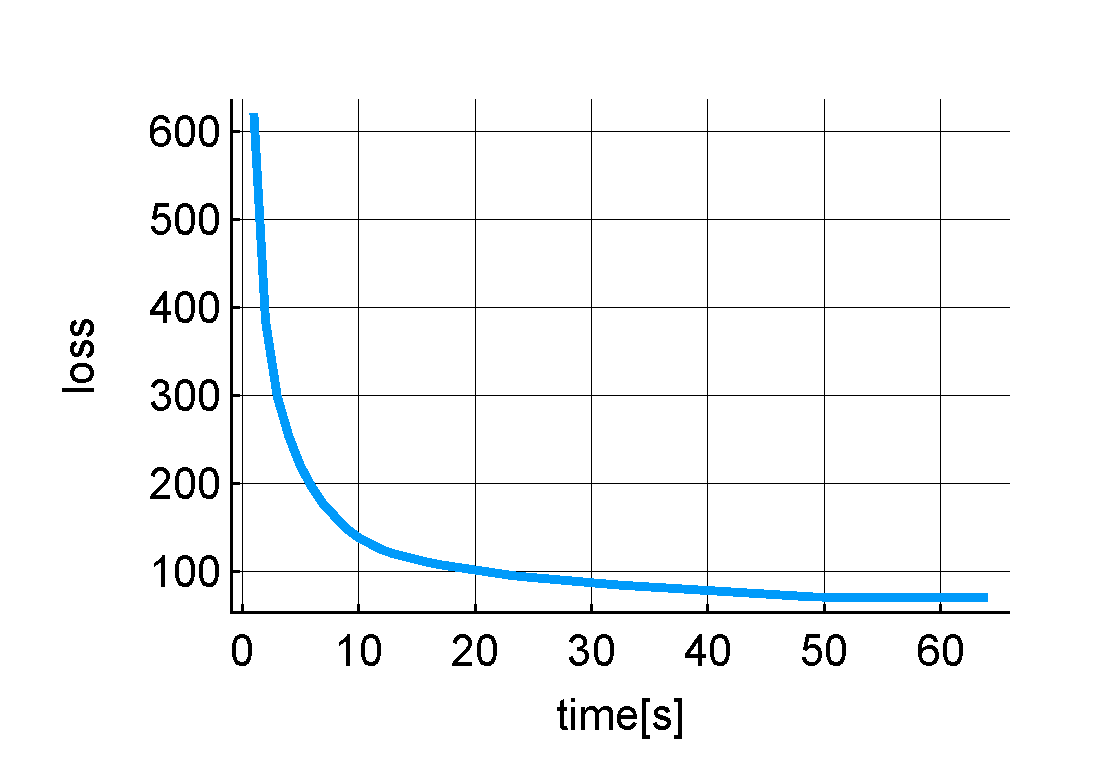
\includegraphics[width=8.0cm]{plots/Images/NCE_loss_2D} }}%
	\subfloat[Comparison of true (blue) and estimated (red) PDF.]
	{{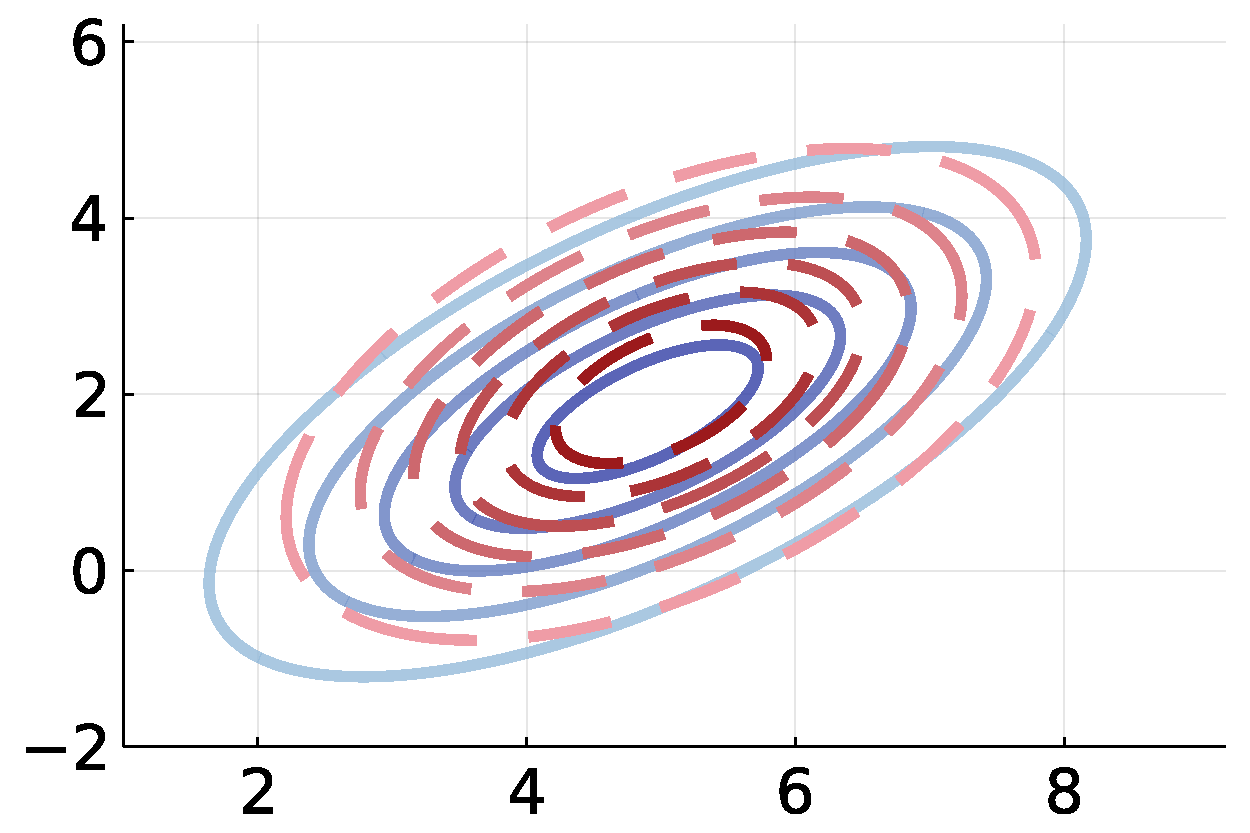
\includegraphics[width=8.0cm]{plots/Images/NCE_results_2D.pdf} }}%
	\caption{Results of the NCE experiment for two--dimensional Gaussian case.}%
	\label{ex:NCE_2}%
\end{figure}

The one--dimensional case may seem too simple, and therefore an example with a two-dimensional Gaussian distribution was performed. The experimental setup remains nearly the same; only the dimensionality of the problem differs. 

Recall that the non--normalized multivariate Gaussian distribution in $\R^2$ can be written as
\begin{equation}
   q_{\bt^\star}\left(\bx\right) = \exp\left(-\frac{1}{2}\left(\boldsymbol{x} - \boldsymbol{\mu}\right)^\top\boldsymbol{\Sigma}^{-1}\left(\boldsymbol{x} - \boldsymbol{\mu}\right)+ c \right),
\end{equation}
where $\boldsymbol{\mu} \in \R^2$ and $\boldsymbol{\Sigma}\in \R^{2\times 2}$ is a symmetric and positive semidefinite covariance matrix. As the noise PDF is chosen 
$\psi\left(\boldsymbol{e}\right)=\pazocal{N}\left(\boldsymbol{e}; \boldsymbol{\mu}_1,\boldsymbol{\Sigma}_1\right)$, where $\boldsymbol{\mu}_1 = \left(2,2\right)^\top$ and $\boldsymbol{\Sigma}_1=10\cdot\mathbb{I}_2$. Figure \ref{ex:NCE_2} shows the results in a similar vein to the previous case.
\end{example}


\chapter{Hybrid Generative and Discriminative models}

\section{Energy-Based Models}\label{EBM}
Energy-based models (EBM) was firstly introduced here \cite{energy}, but following nomenclature was established here \cite{energy2}. EBM assume that probability densities $p(\boldsymbol{x})$ for $\boldsymbol{x} \in \mathbb{R}^D$ can be expressed in the form
\begin{equation}
	p_{\boldsymbol{\theta}}\left(\boldsymbol{x}\right) = \frac{\exp\left(-E_{\boldsymbol{\theta}}(\boldsymbol{x})\right)}{Z(\boldsymbol{\theta})},
\end{equation}
where function $E_{\boldsymbol{\theta}} : \mathbb{R}^D \to \mathbb{R}$ is called Energy and maps each datapoint $\boldsymbol{x}$ to a scalar. The denominator $Z(\boldsymbol{\theta})$ is a normalization constant (also known as partition function), thus
\begin{equation}
	Z(\boldsymbol{\theta}) = \sum_{i=1}^N \exp\left(-E_{\boldsymbol{\theta}}(\boldsymbol{x}_i)\right),
\end{equation}
where  the summation is over all datapoints $\boldsymbol{x}$ available. The sum turns into integral for a continuous $\boldsymbol{x}$.   Very important observations made authors in \cite{energy2}, where they show, that classifiers in supervised learning are secretly energy-based models on $p(\boldsymbol{x},y)$ and can be expressed as
\begin{equation}
	p\left(\boldsymbol{x},y\right) = \frac{\exp\left({f_{\boldsymbol{\theta}}\left(\boldsymbol{x}\right)[y]}\right)}{Z(\boldsymbol{\theta})}.
\end{equation}
The obbjective above is called joint energy model and it is obvious that $f_{\boldsymbol{\theta}}\left(\boldsymbol{x}\right)[y] = -E_{\boldsymbol{\theta}}(\boldsymbol{x},y)$. It may come in handy to have only a density model of datapoints $p(\boldsymbol{x})$ without labels. This could be achieved by marginalizing $p(\boldsymbol{x},y)$ over $y$ 
\begin{equation}
	p\left(\boldsymbol{x}\right) = \frac{\sum_{i=1}^C\exp\left({f_{\boldsymbol{\theta}}\left(\boldsymbol{x}\right)[y_i]}\right)}{Z(\boldsymbol{\theta})},
\end{equation}
where energy is given by $E_{\boldsymbol{\theta}}(\boldsymbol{x}) = -\log\sum_{i=1}^C\exp\left({f_{\boldsymbol{\theta}}\left(\boldsymbol{x}\right)[y_i]}\right)$. Very useful property appears when computing $p(y|\boldsymbol{x})$. We can take advatage of the definition of conditional distribution $p(y|\boldsymbol{x})~=~\frac{p\left(\boldsymbol{x},y\right)}{p\left(\boldsymbol{x}\right)}$, yielding  
\begin{equation}\label{softmaxdef}
	p_{\boldsymbol{\theta}}\left(y|\boldsymbol{x}\right) = \frac{\exp\left({f_{\boldsymbol{\theta}}\left(\boldsymbol{x}\right)[y]}\right)}{\sum_{i=1}^C\exp\left({f_{\boldsymbol{\theta}}\left(\boldsymbol{x}\right)[y_i]}\right)}.
\end{equation}
Note that the normalization constant $Z(\boldsymbol{\theta})$ canceled out and we ended up with the same function, which was introduced in \eqref{softmax}. 
\section{Contrastive learning}
 Contrastive learning \cite{contrastive1, contrastive2} is a ML technique used to learn so-called general features of a dataset by teaching the model which datapoints are similar or different. This all happens without labels, therefore contrastive learning is often called \emph{self--supervised} technique of ML.  In contrastive learning problems, it is very usual to optimize an objective often called contrastive loss, which can be written in the form as follows
\begin{equation}\label{eq:contrastive}
	\min_{\boldsymbol{\theta}}- \mathbb{E}_{p_{\mathrm{data}}(\boldsymbol{x})}\left[\log \frac{\exp\left({h_{\boldsymbol{\theta}}\left(\boldsymbol{x}\right)\cdot h_{\boldsymbol{\theta}}\left(\boldsymbol{x}'\right)}\right)}{\sum_{i=1}^N\exp\left({h_{\boldsymbol{\theta}}\left(\boldsymbol{x}\right)\cdot h_{\boldsymbol{\theta}}(\boldsymbol{x}_i) }\right)} \right].
\end{equation}
Function $h_{\boldsymbol{\theta}}: \mathbb{R}^D \to \mathbb{R}^H$ maps each data point to a representation space with dimension $H$, while $\boldsymbol{x}$ and $\boldsymbol{x}'$ are two different augmented views of the same data point. If $\boldsymbol{x}$ is an image, then augmented view of $\boldsymbol{x}$ can be obtained for example by rotation or colorization of that image. Note that the inner product between two vectors can replaced with any distance metric, for example Euclidean distance. \\
What this objective does is that it tries to maximally distinguish an input $\boldsymbol{x}_i$ from an alternative input $\boldsymbol{x}'_i$. In other words, \eqref{eq:contrastive} reduces the distance between representations of different augmented views of the same image $\boldsymbol{x}, \boldsymbol{x}'$ (positive pairs) and increases the distance between representations of augmented viwes of from different images (negative pairs). This means that the model should be able to distinguish between different types of images without even knowing what these images really are. 
\section{Hybrid Dicriminative and Generative Models, HDGM}
In this section will be discussed an approach, how to combine both of the already mentioned models.
Authors of the article \cite{HDGEmain} proposed a solution, however the rationale of this objective originates from \cite{generativevsdisriminative}, where authors show that hybrid models can out--perform purely generative or purely discriminative counterparts.\\
The primary goal is to train a model that can classify $\boldsymbol{x}$ to classes $y$. Secondarily, learned models should be capable of out-of-distribution detection and serve as a generative model. To achieve these goals, a hybrid model consists of a discriminative conditional and a generative conditional by maximizing the sum of both conditional log-likelihoods
\begin{equation}\label{q1q2}
	\min_{\boldsymbol{\theta}}- \mathbb{E}_{p_{\mathrm{data}}(\boldsymbol{x},y)}\left[\log q_{\boldsymbol{\theta}}\left(y|\boldsymbol{x}\right)+ \log q_{\boldsymbol{\theta}}\left(\boldsymbol{x}|y\right) \right],
\end{equation}
where the first term 
\begin{equation}
q_{\boldsymbol{\theta}}\left(y|\boldsymbol{x}\right) = \frac{\exp\left({f_{\boldsymbol{\theta}}\left(\boldsymbol{x}\right)[y]}\right)}{\sum_{i=1}^C\exp\left({f_{\boldsymbol{\theta}}\left(\boldsymbol{x}\right)[y_i]}\right)}
\end{equation}

is a standard Softmax neural net classifier (as mentioned in Equation \eqref{softmax}) and the second term 
\begin{equation}
	q_{\boldsymbol{\theta}}\left(\boldsymbol{x}|y\right) = \frac{\exp\left({f_{\boldsymbol{\theta}}\left(\boldsymbol{x}\right)[y]}\right)}{\sum_{j=1}^N\exp\left({f_{\boldsymbol{\theta}}\left(\boldsymbol{x}_j\right)[y]}\right)},
\end{equation}
is a contrastive loss \eqref{eq:contrastive} attributed a label. This objective  often struggles with the unknown partition function $\sum_{j=1}^N\exp\left({f_{\boldsymbol{\theta}}\left({\boldsymbol{x}_j}\right)[y]}\right)$, which is often intractable, specifically if the number of datapoints is very high. This obstacle is typically addressed using an approximation 
\begin{align}\label{approxcontrasstive}
	&\mathbb{E}_{p_{\mathrm{data}}(\boldsymbol{x},y)}\left[ \log q_{\boldsymbol{\theta}}\left(\boldsymbol{x}|y\right) \right] \\
	&=\mathbb{E}_{p_{\mathrm{data}}(\boldsymbol{x},y)}\left[\log \frac{\exp\left({f_{\boldsymbol{\theta}}\left(\boldsymbol{x}\right)[y]}\right)}{\sum_{j=1}^N\exp\left({f_{\boldsymbol{\theta}}\left(\boldsymbol{x}_j\right)[y]}\right)} \right]  \\
	&\approx\mathbb{E}_{p_{\mathrm{data}}(\boldsymbol{x},y)}\left[\log \frac{\exp\left({f_{\boldsymbol{\theta}}\left(\boldsymbol{x}\right)[y]}\right)}{\sum_{j=1}^M\exp\left({f_\theta\left(\boldsymbol{x}_j\right)[y]}\right)} \right],
\end{align}
where $M < N$ denotes the number of normalization samples. In order to have an sufficient approximation, $M$ has to be sufficiently large - becoming exact in the limit $M \to N$. In practice, increasing $M$ is not simple as it requires a larger memory. However, that does not apply to our experiments. \\
Now it is possible to substitute approximation \eqref{approxcontrasstive} to Equation \eqref{q1q2} that gives a hybrid combination of supervised learning and constrastive learning in the form
\begin{align}\label{eq:q1q2final}
	&\min_{\boldsymbol{\theta}}- \mathbb{E}_{p_{\mathrm{data}}(\boldsymbol{x},y)}\left[\alpha\log q_{\boldsymbol{\theta}}\left(y|\boldsymbol{x}\right)+ \left(1-\alpha\right)\log q_{\boldsymbol{\theta}}\left(\boldsymbol{x}|y\right) \right]  \\
	&\label{eq:hybrid}\approx	\min_{\boldsymbol{\theta}}- \mathbb{E}_{p_{\mathrm{data}}(\boldsymbol{x},y)}\left[\alpha\log \frac{\exp\left({f_{\boldsymbol{\theta}}\left(\boldsymbol{x}\right)[y]}\right)}{\sum_{i=1}^C\exp\left({f_{\boldsymbol{\theta}}\left(\boldsymbol{x}\right)[y_i]}\right)}+ \left(1-\alpha\right)\log \frac{\exp\left({f_{\boldsymbol{\theta}}\left(\boldsymbol{x}\right)[y]}\right)}{\sum_{i=1}^M\exp\left({f_{\boldsymbol{\theta}}\left(\boldsymbol{x}_i\right)[y]}\right)} \right]. 
\end{align}
Parameter $\alpha$ is a weight between $\left[0,1\right]$. It is obvious that in the case of $\alpha = 1$, the objective reduces to the standard cross entropy loss, while $\alpha = 0$, the objective is reduced to a case called an \emph{end-to-end supervised version of contrastive learning}. The choice of parameter $\alpha$ is a decision of the experiment designer, however authors in \cite{HDGEmain} evaluated many possible variants in performed experiments and found out that the choice of $\alpha=0.5$ yields to the highest performance on a classification accuracy. As far as we know, these experiments involved only image classification, unfortunately. \\
Hybrid combination of supervised learning and contrastive learning \eqref{eq:hybrid} is for us absolutely crucial as we extend this approach to multiple instance learning problem, but this is discussed more in further sections.  


\section{Toy problem - Polynomial Regression}
At first, we would like to try out hybrid discriminative and generative approach on simple example before we head into more difficult cases. The goal is to train a model of the form \eqref{eq:hybrid} that was derived in previous section.\\
Assume data $\left\lbrace x_i,y_i \right\rbrace_{i=1}^N$, where $x_i,y_i\in \R$, therefore this is only 2-dimensional problem.  According to energy--based models \ref{EBM}, we know that for joint distribution it holds
\begin{equation}
	p(x,y) = \frac{\exp{\left(f_{\boldsymbol{\theta}}(x)[y]\right)}}{Z(\boldsymbol{\theta})},
\end{equation}
where the model model is given by 
\begin{equation}
	f_{\boldsymbol{\theta}}(x)[y] = -E_{\boldsymbol{\theta}}(x,y) .
\end{equation}
At this point, we should transform our problem to the polynomial regression. We need to be aware of the discriminative term in the Equation \eqref{q1q2}, because we do not want to classify, but we would like to find the best fit to the given data. For this reason, we replace that with the typical regression loss
\begin{equation}\label{S(theta)}
	S = S(\boldsymbol{\theta}) = \sum_{k=1}^N \left(y_k - \sum_{i=0}^{s-1} \theta_i x^i_k\right)^2.
\end{equation}	
Any joint probability distribution can be break down into parts via chain-rule 
\begin{equation}\label{eq:chainrule}
	p(x,y) =	p(y,x) = p(y\vert x)\cdot p(x),
\end{equation}
thus we need to find $p(y\vert x)$ and $p(x)$. From polynomial regression we can obtain conditional probability density 
\begin{equation}\label{eq:linregpdf}
	p(y\vert x, \boldsymbol{\theta}) = \pazocal{N}\left(\sum_{i=0}^{s-1} \theta_i x^i, \sigma^2 \right),
\end{equation}
where symbol $\pazocal{N}(\cdot)$ denotes probability density function of Normal distribution and $\sigma^2$ is known variance. In this case, we also need to determine prior distribution on $x$. To keep this example simple, let the pdf takes the form
\begin{equation}\label{eq:tauprior}
	p(x|\tau) = \pazocal{N}\left(0, \tau^2\right),
\end{equation}
where the choice of parameter $\tau$ is based on the fact that we would like to have a non--informative prior, thus $\tau$ should be adequately high. If the value of $\tau$ is high, data are spread very far from their expected value.  Subtituting Equation \eqref{eq:tauprior} and \eqref{eq:linregpdf} to the \eqref{eq:chainrule} results to
\begin{equation}
	p(x,y) = \pazocal{N}\left(0,\tau^2\right) \cdot \pazocal{N}\left(\sum_{i=0}^{s-1} \theta_i x^i, \sigma^2 \right)  =  \frac{1}{2\pi\sigma\tau}\exp\left(-\frac{\left(y-\sum_{i=0}^{s-1} \theta_i x^i\right)^2}{2\sigma^2}-\frac{x^2}{2\tau^2}\right),
\end{equation}
whereas our desirable model is given by
\begin{equation}\label{modelflinreg}
	f_{\boldsymbol{\theta}}(x)[y] = -\frac{\left(y-\sum_{i=0}^{s-1} \theta_i x^i\right)^2}{2\sigma^2} - \frac{x^2}{2\tau^2}.
\end{equation}
We can now substite \eqref{modelflinreg} and \eqref{S(theta)} into Equation \eqref{q1q2}, yielding
\begin{align}\label{eq:SSEq}
	&\min_{\boldsymbol{\theta}}\Big\lbrace \alpha~S(\boldsymbol{\theta}) - \mathbb{E}_{p_{\mathrm{data}}(x,y)}\left[ \left(1-\alpha\right)\log q_{\boldsymbol{\theta}}\left(x|y\right) \right] \Big\rbrace  =\\
	&\min_{\boldsymbol{\theta}}\Bigg\lbrace \alpha~S(\boldsymbol{\theta}) - \mathbb{E}_{p_{\mathrm{data}}(x,y)}\left[ \left(1-\alpha\right)\log \frac{\exp\left({f_{\boldsymbol{\theta}}\left(x\right)[y]}\right)}{\sum_{i=1}^N\exp\left({f_{\boldsymbol{\theta}}\left(x_i\right)[y]}\right)} \right] \Bigg\rbrace  =\\
	&\min_{\boldsymbol{\theta}}\left\lbrace \alpha~S(\boldsymbol{\theta}) - \mathbb{E}_{p_{\mathrm{data}}(x,y)}\left[ \left(1-\alpha\right)\log \frac{\exp\left({-\frac{\left(y- \sum_{i=0}^{s-1} \theta_i x^i     \right)^2}{2\sigma^2} - \frac{x^2}{2\tau^2}}\right)}{\sum_{k=1}^N\exp\left({-\frac{\left(y-\sum_{i=0}^{s-1} \theta_i x_k^i\right)^2}{2\sigma^2} - \frac{x_k^2}{2\tau^2}}\right)} \right] \right\rbrace.  
\end{align}
Finally, we simplify the generative term $\log q_{\boldsymbol{\theta}}\left(x|y\right)$ into
\begin{equation}
	\log q_{\boldsymbol{\theta}}\left(x|y\right) =  \left(-\frac{\left(y-\sum_{i=0}^{s-1} \theta_i x^i\right)^2}{2\sigma^2} - \frac{x^2}{2\tau^2}\right) - \log \sum_{k=1}^N\exp\left({-\frac{\left(y-\sum_{i=0}^{s-1} \theta_i x_k^i\right)^2}{2\sigma^2} - \frac{x_k^2}{2\tau^2}}\right).
\end{equation}
Note that for $\alpha =1$ we get purely polynomial regression and for $\alpha =0$, the term $S(\boldsymbol{\theta})$ is not involved at all. Now, we have everything we need to perform the experiment.
\subsection{Experiment setup and results}
We would like to test the sensitivity of this approach on the unknown parameter $\tau$ and order of the polynomial $s-1$. In addition, we would like to observe, how the estimated model behaves in relation to $\alpha$. \\
We generated synthetic data, two clusters consisting of 5 datapoints each, then the model was fitted for different weight $\alpha \in \left\{0.0, 0.1, 0.2,\dots,1.0\right\}$, giving 11 different models in total. Models estimated for $\alpha \in \left\{0.0, 0.5, 1.0 \right\}$ are highlighted as they are more important to us then the other models.\\
At first, we trained the mentioned models for the fixed order of the polynomial, but for 6 different values of the parameter $\tau$. Obtained results (Figure \ref{fig:linregtoy_tau}) for small $\tau$ barely vary from those for high $\tau$, that is exactly what we hoped for, since the prior distribution should be non--informative \eqref{eq:tauprior}.  This is very exciting discovery, because there is no need to know much information about the data distribution.\\
Secondly, we trained our polynomial models for the fixed value of $\tau$ with 6 different values of the order of the polynomial. The goal of this part of the experiment is to observe how the contrastive part of Equation \eqref{eq:SSEq} affects the polynomial regression loss for different values of $s-1$. As can be seen in Figure \ref{fig:linregtoy_s}, for small $s-1$, such as $s-1 = 2$, term $\log q_{\theta}\left(x|y\right)$ does not affect polynomial regression too much. However, we get considerable difference for higher orders of the polynomial. Furthermore, it seems that the curve $\alpha = 0$ prefers not to oscillate. This also could be very interesting, because combining of discriminative and generative models could result in better model predictions.    

\begin{figure}[h] 
	\centering
	\subfloat[Estimated model for $\tau=1$ and $s=11$.]
	{{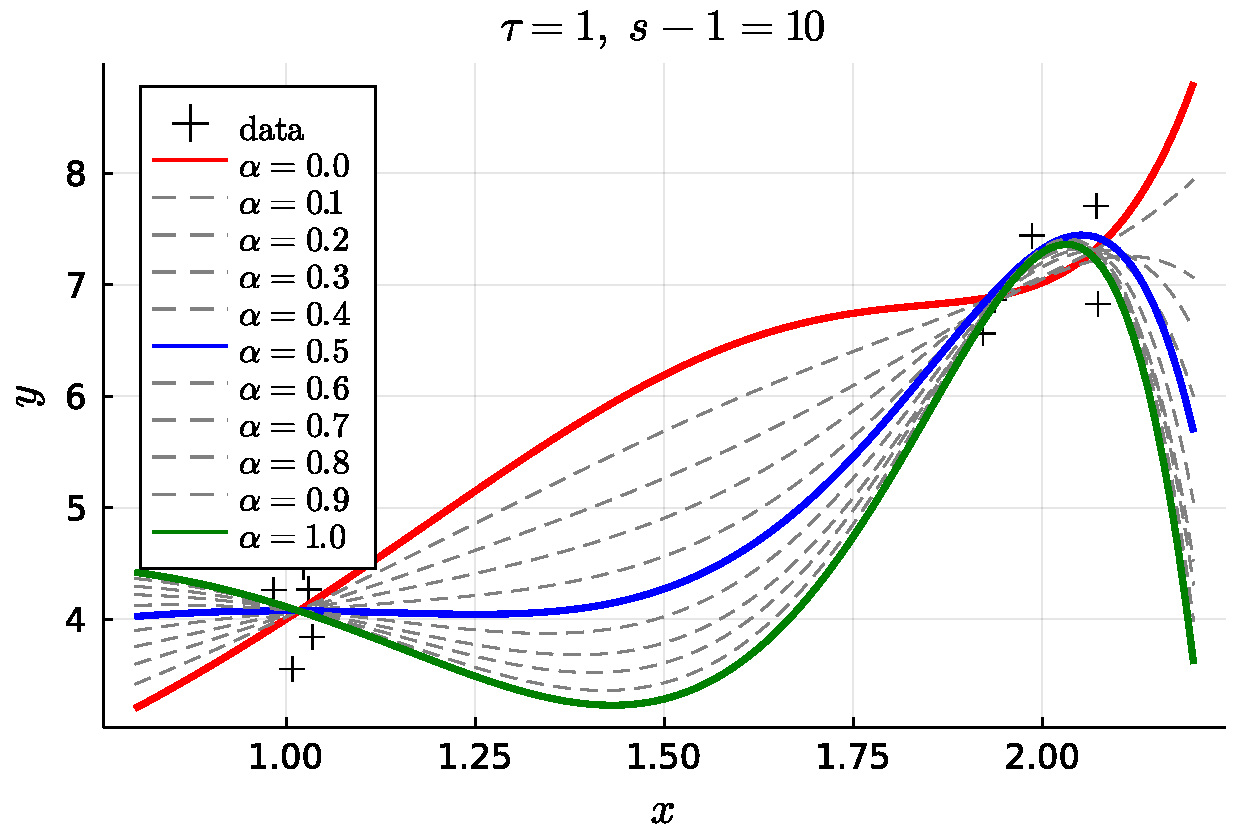
\includegraphics[width=8.0cm]{plots/Images/tau1.pdf} }}%
	\subfloat[Estimated model for $\tau=10$ and $s=11$.]
	{{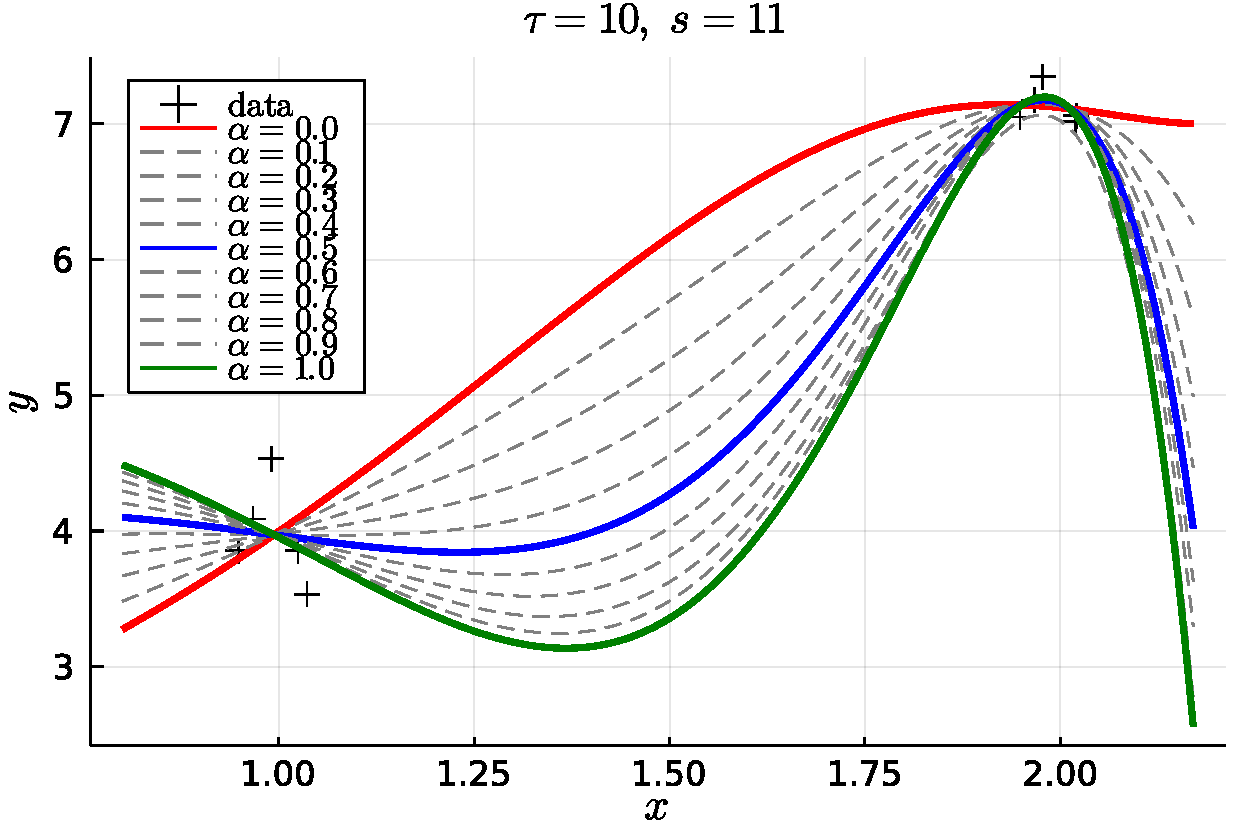
\includegraphics[width=8.0cm]{plots/Images/tau10.pdf} }}%
	\
	\subfloat[Estimated model for $\tau=100$ and $s=11$.]
	{{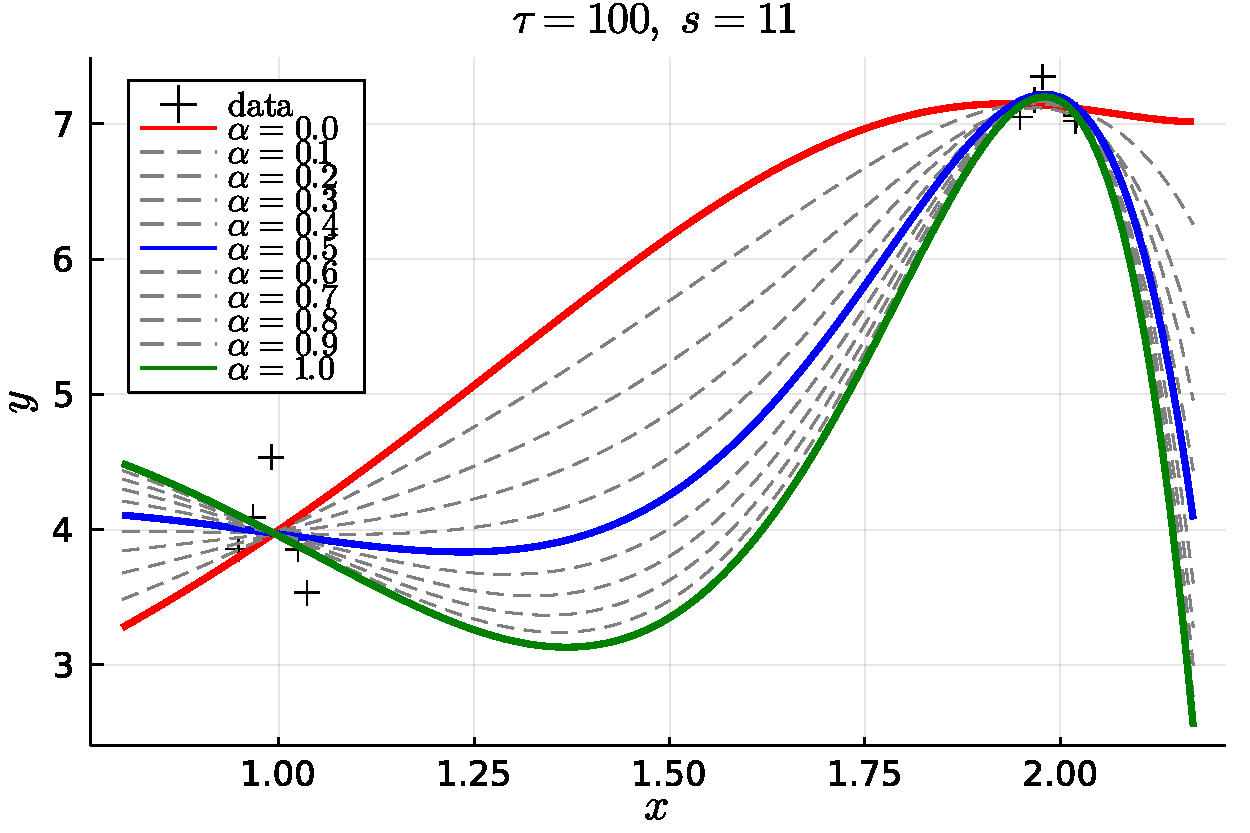
\includegraphics[width=8.0cm]{plots/Images/tau100.pdf} }}%,
	\subfloat[Estimated model for $\tau=1000$ and $s=11$.]
	{{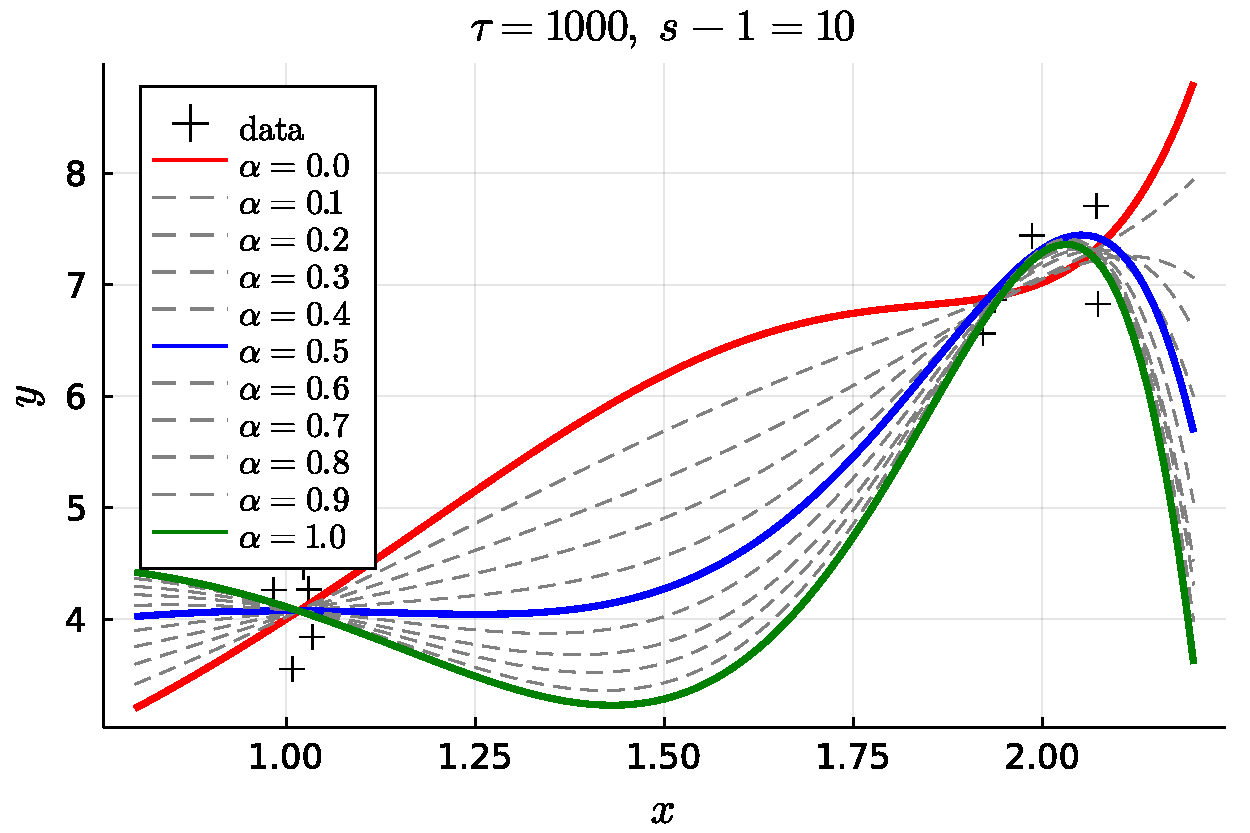
\includegraphics[width=8.0cm]{plots/Images/tau1000.pdf} }}%
	\
	\subfloat[Estimated model for $\tau=100000$ and $s=11$.]
	{{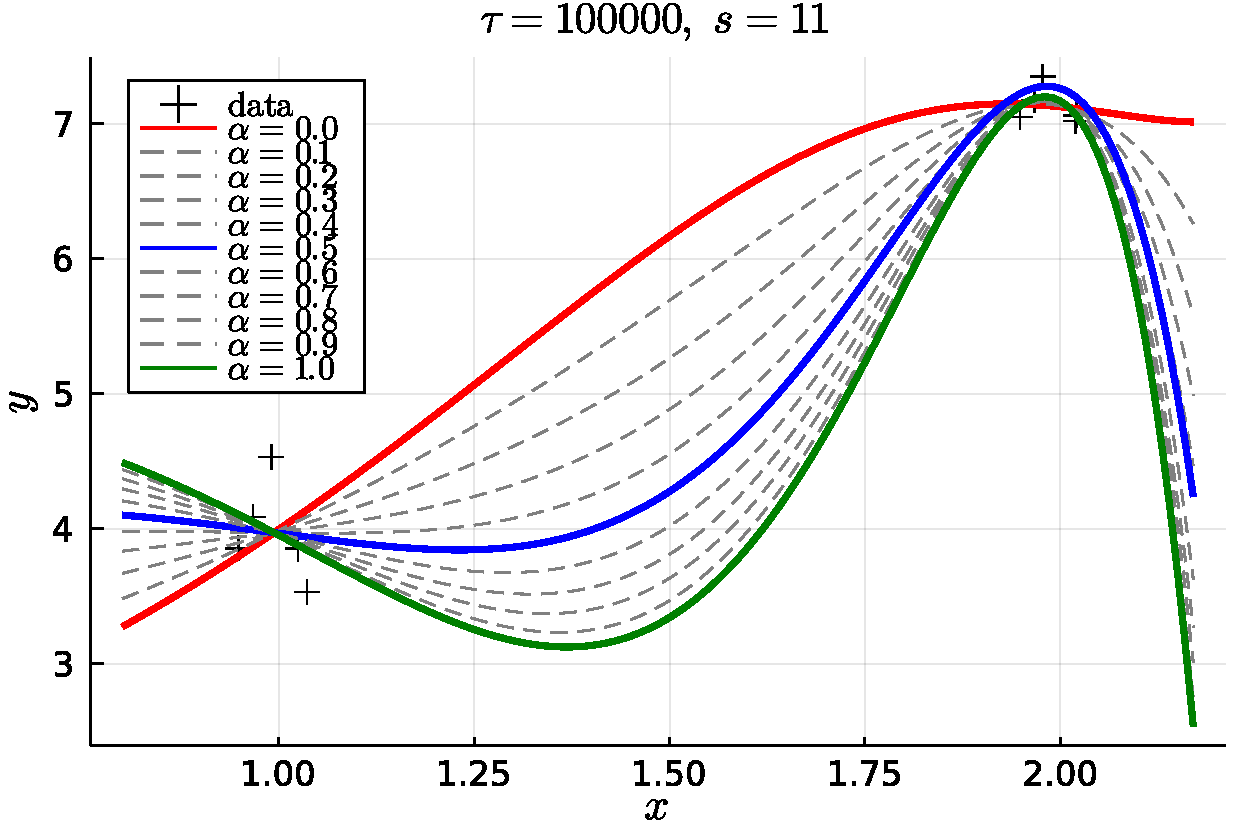
\includegraphics[width=8.0cm]{plots/Images/tau100000.pdf} }}%,
	\subfloat[Estimated model for $\tau=1000000$ and $s=11$.]
	{{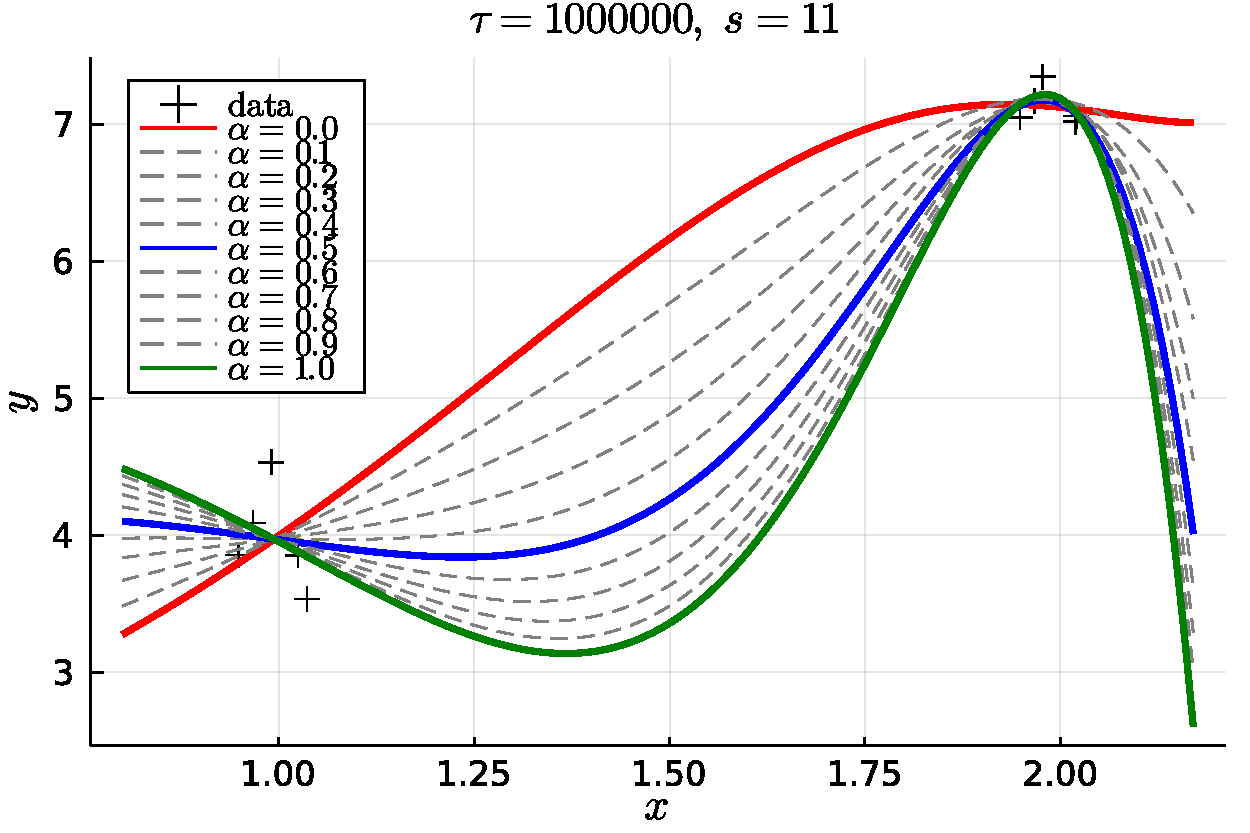
\includegraphics[width=8.0cm]{plots/Images/tau1000000.pdf} }}%
	\caption{Sensitivity of the polynomial model to parameter $\tau$ with parameter $s$ held fixed for six different cases.}%
	\label{fig:linregtoy_tau}%
\end{figure}

\begin{figure}[h]
	\centering
	\subfloat[Estimated model for $\tau=100$ and $s-1=2$.]
	{{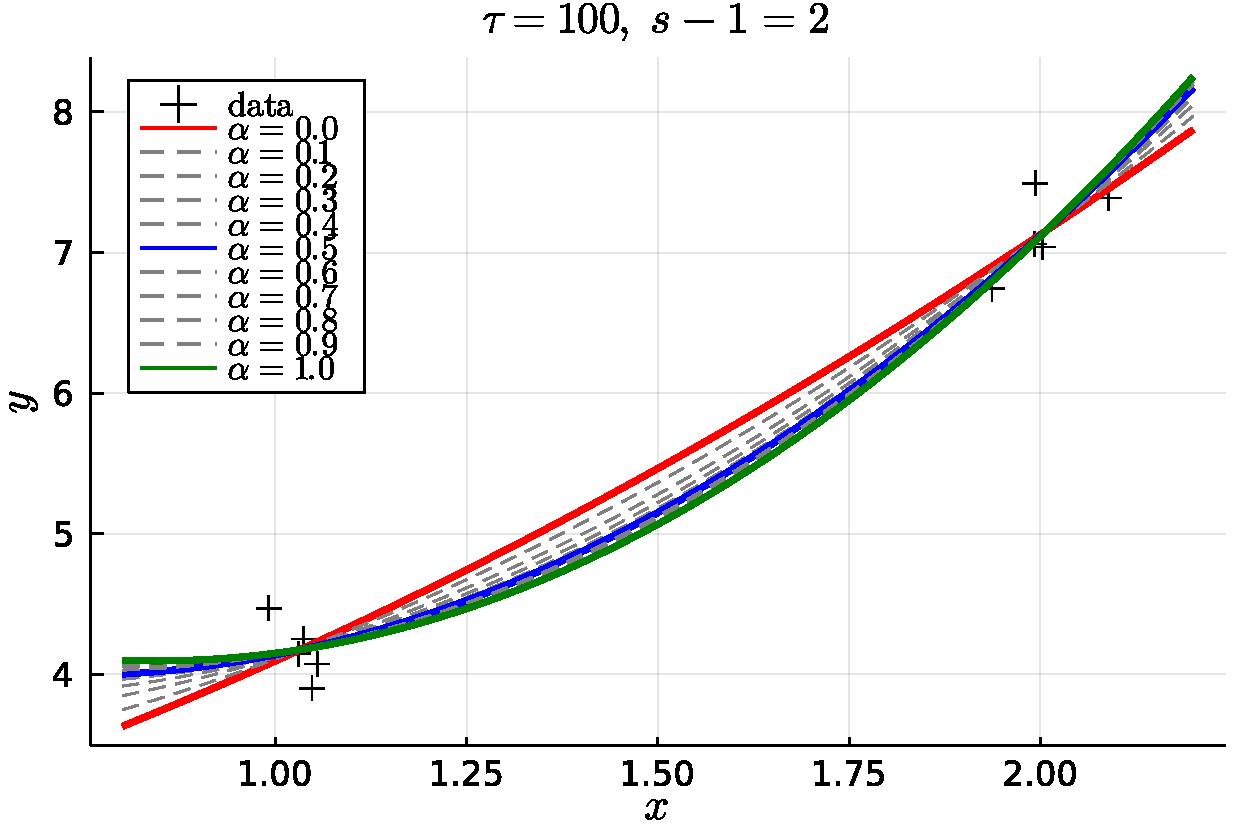
\includegraphics[width=8.0cm]{plots/Images/n2.pdf} }}%
	\subfloat[Estimated model for $\tau=100$ and $s-1=4$.]
	{{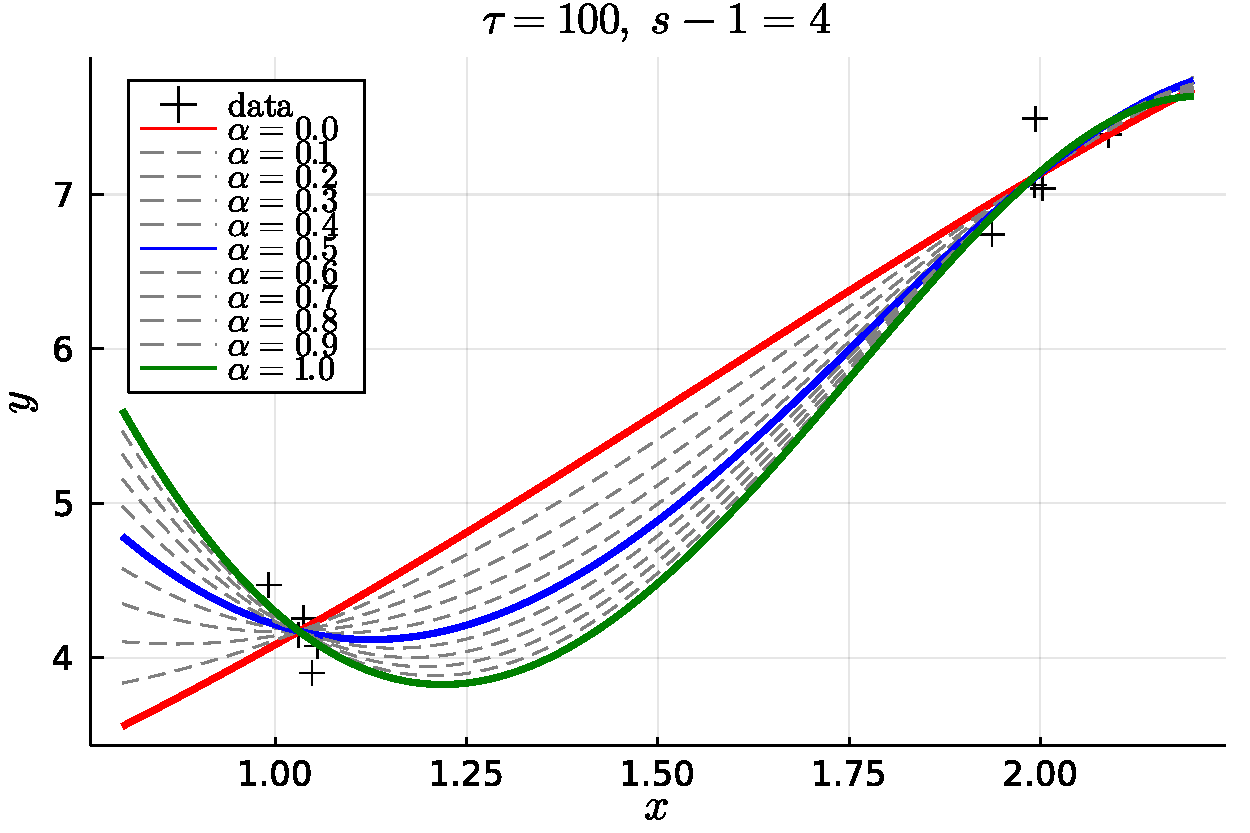
\includegraphics[width=8.0cm]{plots/Images/n4.pdf} }}%
	\
	\subfloat[Estimated model for $\tau=100$ and $s-1=5$.]
	{{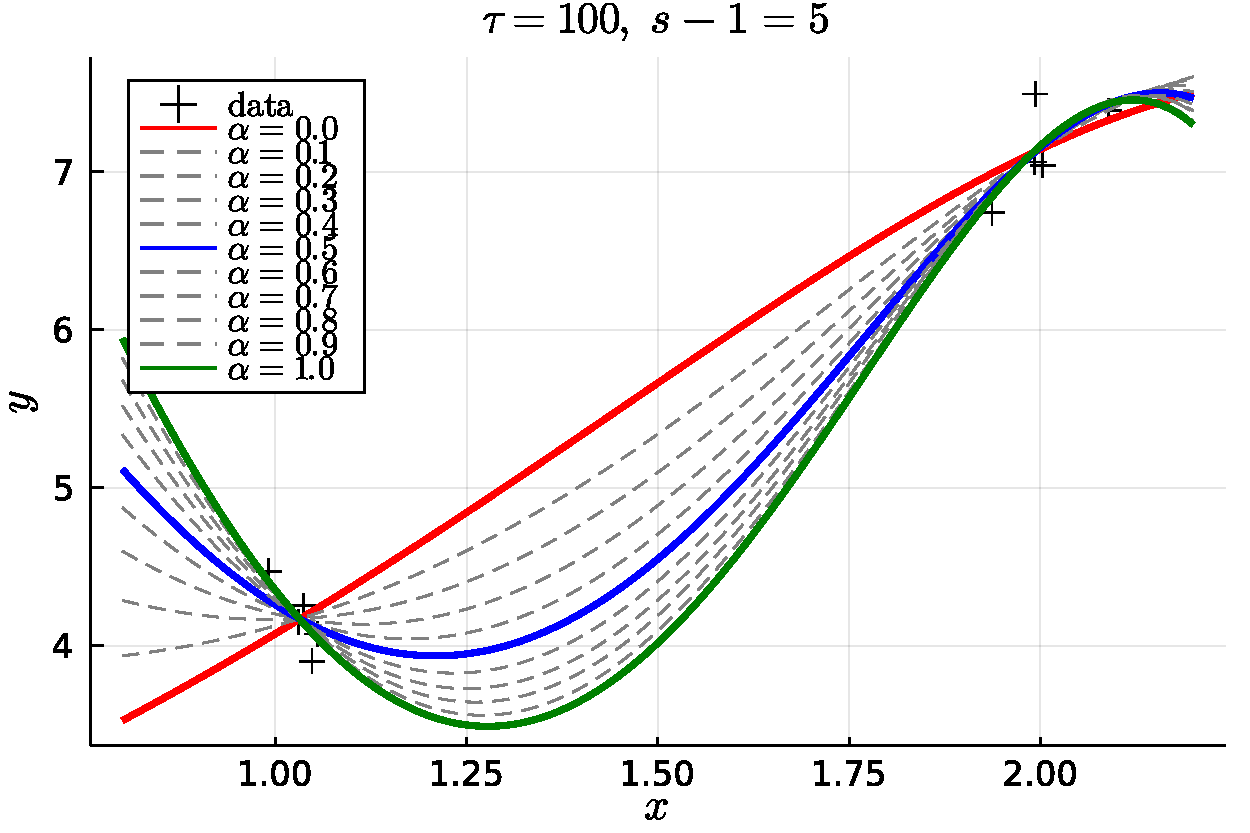
\includegraphics[width=8.0cm]{plots/Images/n5.pdf} }}%,
	\subfloat[Estimated model for $\tau=100$ and $s-1=6$.]
	{{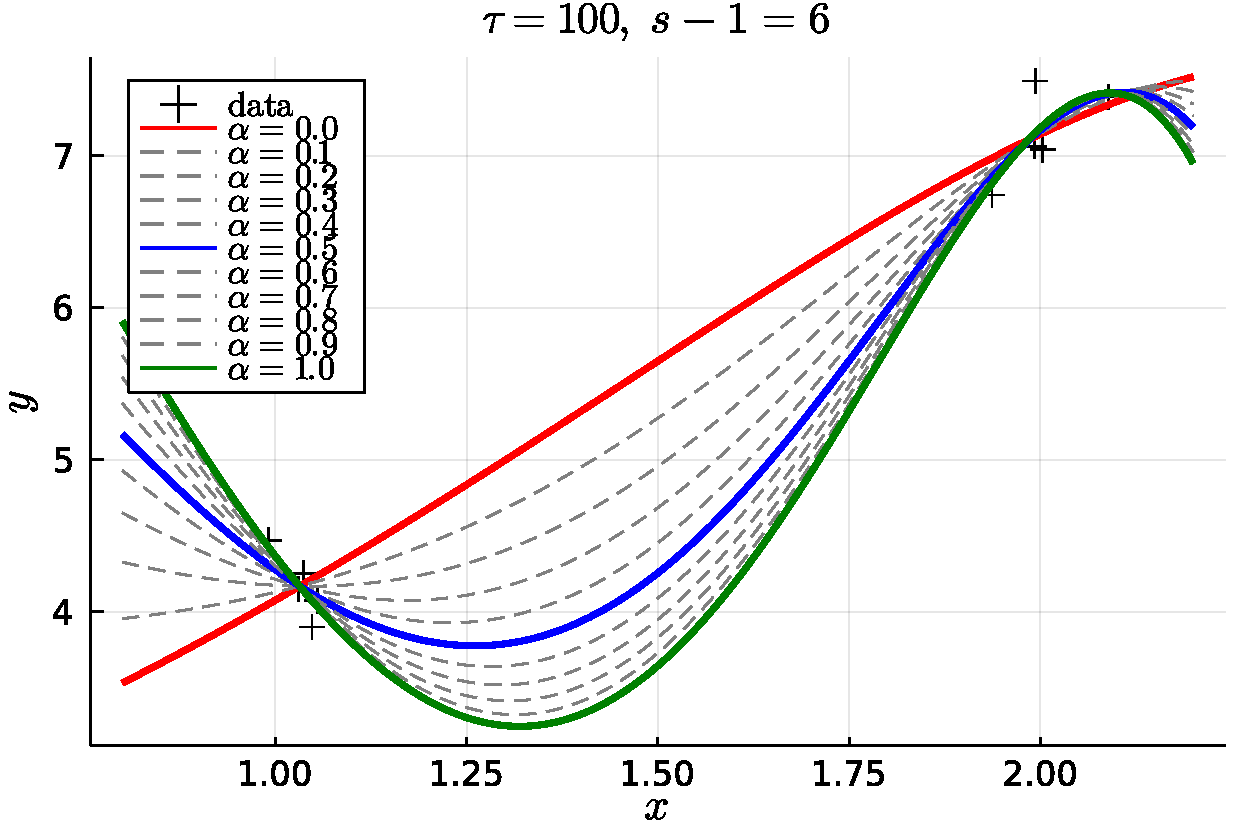
\includegraphics[width=8.0cm]{plots/Images/n6.pdf} }}%
	\
	\subfloat[Estimated model for $\tau=100$ and $s-1=8$.]
	{{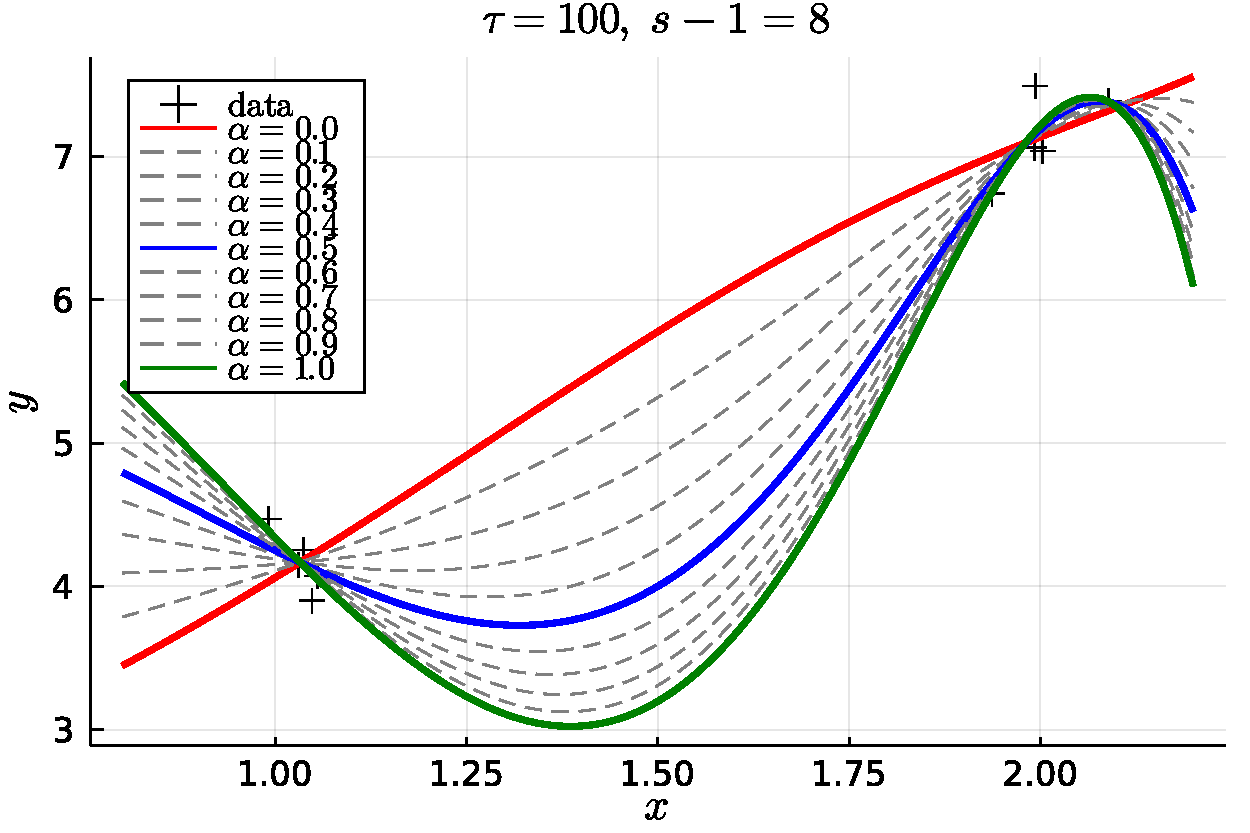
\includegraphics[width=8.0cm]{plots/Images/n8.pdf} }}%,
	\subfloat[Estimated model for $\tau=100$ and $s-1=10$.]
	{{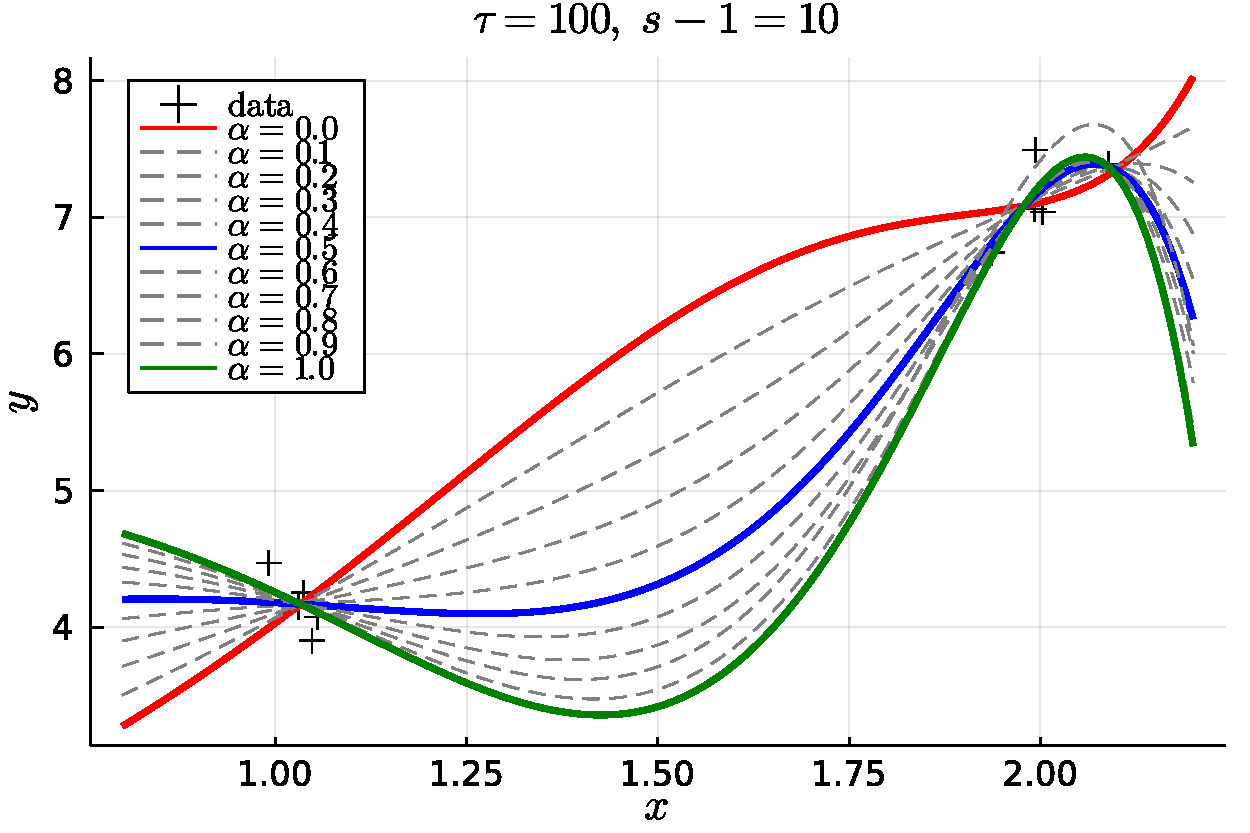
\includegraphics[width=8.0cm]{plots/Images/n10.pdf} }}%
	\caption{Sensitivity of the polynomial model to the order of polynomial $s-1$ for six different cases.}%
	\label{fig:linregtoy_s}%
\end{figure}

\chapter{Multiple Instance Learning}
\section{Fundamentals}
The term multiple instance learning originates from \cite{MILfirstly} and in \cite{mandlik}, authors proposed following nomenclature for MIL, which will be reviewed and gladly used in our work. \\
In standard machine learning problems each sample is represented by a fixed vector $\boldsymbol{x}$ of observations, however in multiple instance learning (MIL) it is dealt with samples which are represented by a set of vectors. These vectors are called \emph{instances} and come from an instance space $\pazocal{X}$, for example $\mathbb{R}^n$. Sets of these instances are called \emph{bags} and come from bag space $\pazocal{B} = \pazocal{P}_F\left(\pazocal{X}\right)$, where $\pazocal{P}_F\left(\pazocal{X}\right)$ denotes all finite subsets of $\pazocal{X}$. With this in mind, we can easily write down any bag as $b = \left\lbrace \boldsymbol{x} \in  \pazocal{X} \right\rbrace_{\boldsymbol{x} \in b}$. Each bag $b$ can be arbitrarily large or empty thus the size of bag is defined in the form $\vert b\vert \in \mathbb{N}_0$. There may exist intrinsic labeling of instances, but we are only interested in labeling at the bag levels. Bag labels come from a finite set $\pazocal{C}$ and what we want in MIL is learning a predictor in the form $f_{\boldsymbol{\theta}}: \pazocal{B}\left(\pazocal{X}\right) \rightarrow \pazocal{C}$ which can also be rewritten in the form $f_{\boldsymbol{\theta}}\left(\left\lbrace \boldsymbol{x}\right\rbrace_{\boldsymbol{x}\in b}\right)$. In contrast to ML, where a predictor is learned in the form  $f_{\boldsymbol{\theta}}: \mathbb{R}^n \rightarrow \pazocal{C}$.  We consider supervised setting, in which each sample of the dataset is attributed a label. We can denote available data by notation $\pazocal{D} = \Big\lbrace \left(b_i, y_i\right) \in \pazocal{B}\times\pazocal{C} \ | \ i \in \big\lbrace 1,2,\dots,\vert \pazocal{D} \vert \big\rbrace \Big\rbrace$, where $\vert \pazocal{D} \vert$ apparently denotes the size of $\pazocal{D}$. 
\begin{figure}[h]
	\centering
	\subfloat[Standard machine learning]
	{{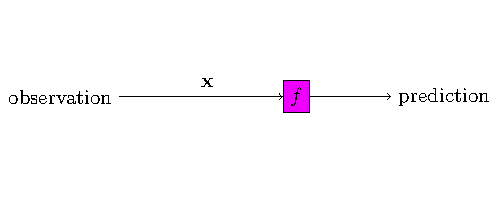
\includegraphics[width=8.0cm]{plots/Images/tikzit_image1} }}%
	\subfloat[Multiple instance learning]
	{{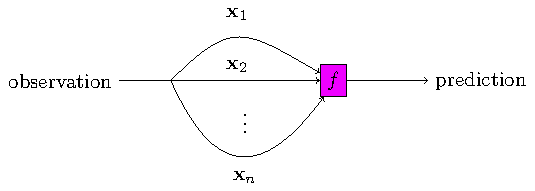
\includegraphics[width=8.0cm]{plots/Images/tikzit_image3} }}%
	\caption{The difference between standard ML and MIL \cite{mandlik}. Standard ML is special case of MIL with $\vert b \vert = 1$. }%
	\label{ggm}%
\end{figure}
\section{Embedded-space paradigm}
Embedded space paradigm \cite{mandlik} defines a vector space for bag representation and specify a mapping from each bag $b\in \pazocal{B}$ to this space. Assume that target vector space is $\R^d$, then partial mapping $\phi_i$: $\pazocal{B} \to \R,~~\forall i=1,2\dots d$~~is defined and overall embedding $\boldsymbol{\phi}: \pazocal{B} \to \R^d $ is given by
\begin{equation}
	\boldsymbol{\phi}(b) = \left(\phi_1(b), \phi_2(b), \dots, \phi_d(b)\right).
\end{equation}
Mappings $\phi_i$ are instrumentals towards extraction and suitable aggregation of information on the level of instances. They can be defined via some instance transformation $k:\pazocal{X}\to \R^d$ and aggregation function $g:\pazocal{P}_F\left(\R^d\right) \to \R^s$ in the form 
\begin{equation}
	\phi_i(b)=g\left( k\left\lbrace\boldsymbol{x}\right\rbrace_{\boldsymbol{x} \in b}\right).
\end{equation}
On the resulting embedded representation of bag samples can be applied any standard machine learning algorithm, which is training bag-level classifier $f_{\boldsymbol{\theta}}^B :\R^s \to \pazocal{C}$ using adjusted dataset $D_{\mathrm{ES}}~=~\Big\lbrace \left(\phi(b_i), y_i\right)~\in~\R^s\times\pazocal{C}~\ ~|~\ i~\in~\big\lbrace 1,2,\dots,\vert D\vert\big\rbrace\Big\rbrace$. The most used aggregation functions are minimum, maximum or mean value.
\section{Training}\label{MILtraining}
Authors of \cite{mandlik} proposed a versatile, unified framework called HMill (Hierarchical multi--instance learning library) for model definition, training and even implemented this functionality in \emph{Julia} programming language. Furthermore, the framework was published as an open--source project entitled \emph{Mill.jl} under MIT license. The aim of this work does not lie in rigorous derivation of the MIL model, since it is fairly complicated and requires considerable amount of work. Considering that, we settle with the MIL model being a neural network (NN) utilizing aggregation functions on the level of instances and we refer to \cite{mandlik} for more details about the model definition and its composition.   \\
Learning of the MIL model $f_{\boldsymbol{\theta}}$ is also supervised, a specific case called binary classification, and therefore accomplished by minimizing standard cross--entropy 
\begin{equation}\label{crossentropy52}
	\min_{\boldsymbol{\theta}}- \mathbb{E}_{p_{\mathrm{data}}(\boldsymbol{x},y) }\left[\log \frac{\exp\left({f_{\boldsymbol{\theta}}\left(\boldsymbol{x}\right)[y]}\right)}{\sum_{i=1}^C\exp\left({f_{\boldsymbol{\theta}}\left(\boldsymbol{x}\right)[y_i]}\right)} \right],
\end{equation}   
already mentioned in section \ref{discriminative_modelinmg}. This is very important for us and we will take advantage of that in our experiments.
 
\section{Cross--validation on MIL datasets}\label{experimentCV}
For testing MIL, we have available four datasets, namely Musk1, Musk2, Tiger and Fox. All of them will be used to assess performance of the MIL model.
\subsection{Setup}
In this experiment, datasets are 100 times randomly split into 2 sets in advance, train and test sets, with 80\% of observations being in train set and 20\% of observations belonging to test set. For a future simplification, let a number of random splits be denoted by $r$, thus $r=100$.  We fit the model on train set, then we evaluate the prediction error on the train data via cross--entropy \ref{crossentropy}. The objective here is to plot the prediction error dependency on the model complexity. Smaller number of random splits $r$ were tested, but obtained results were too noisy. For this reason, such high $r$ was selected, although the experiment became noticeably expensive to compute.    \\

\begin{figure}[h]
	\centering
	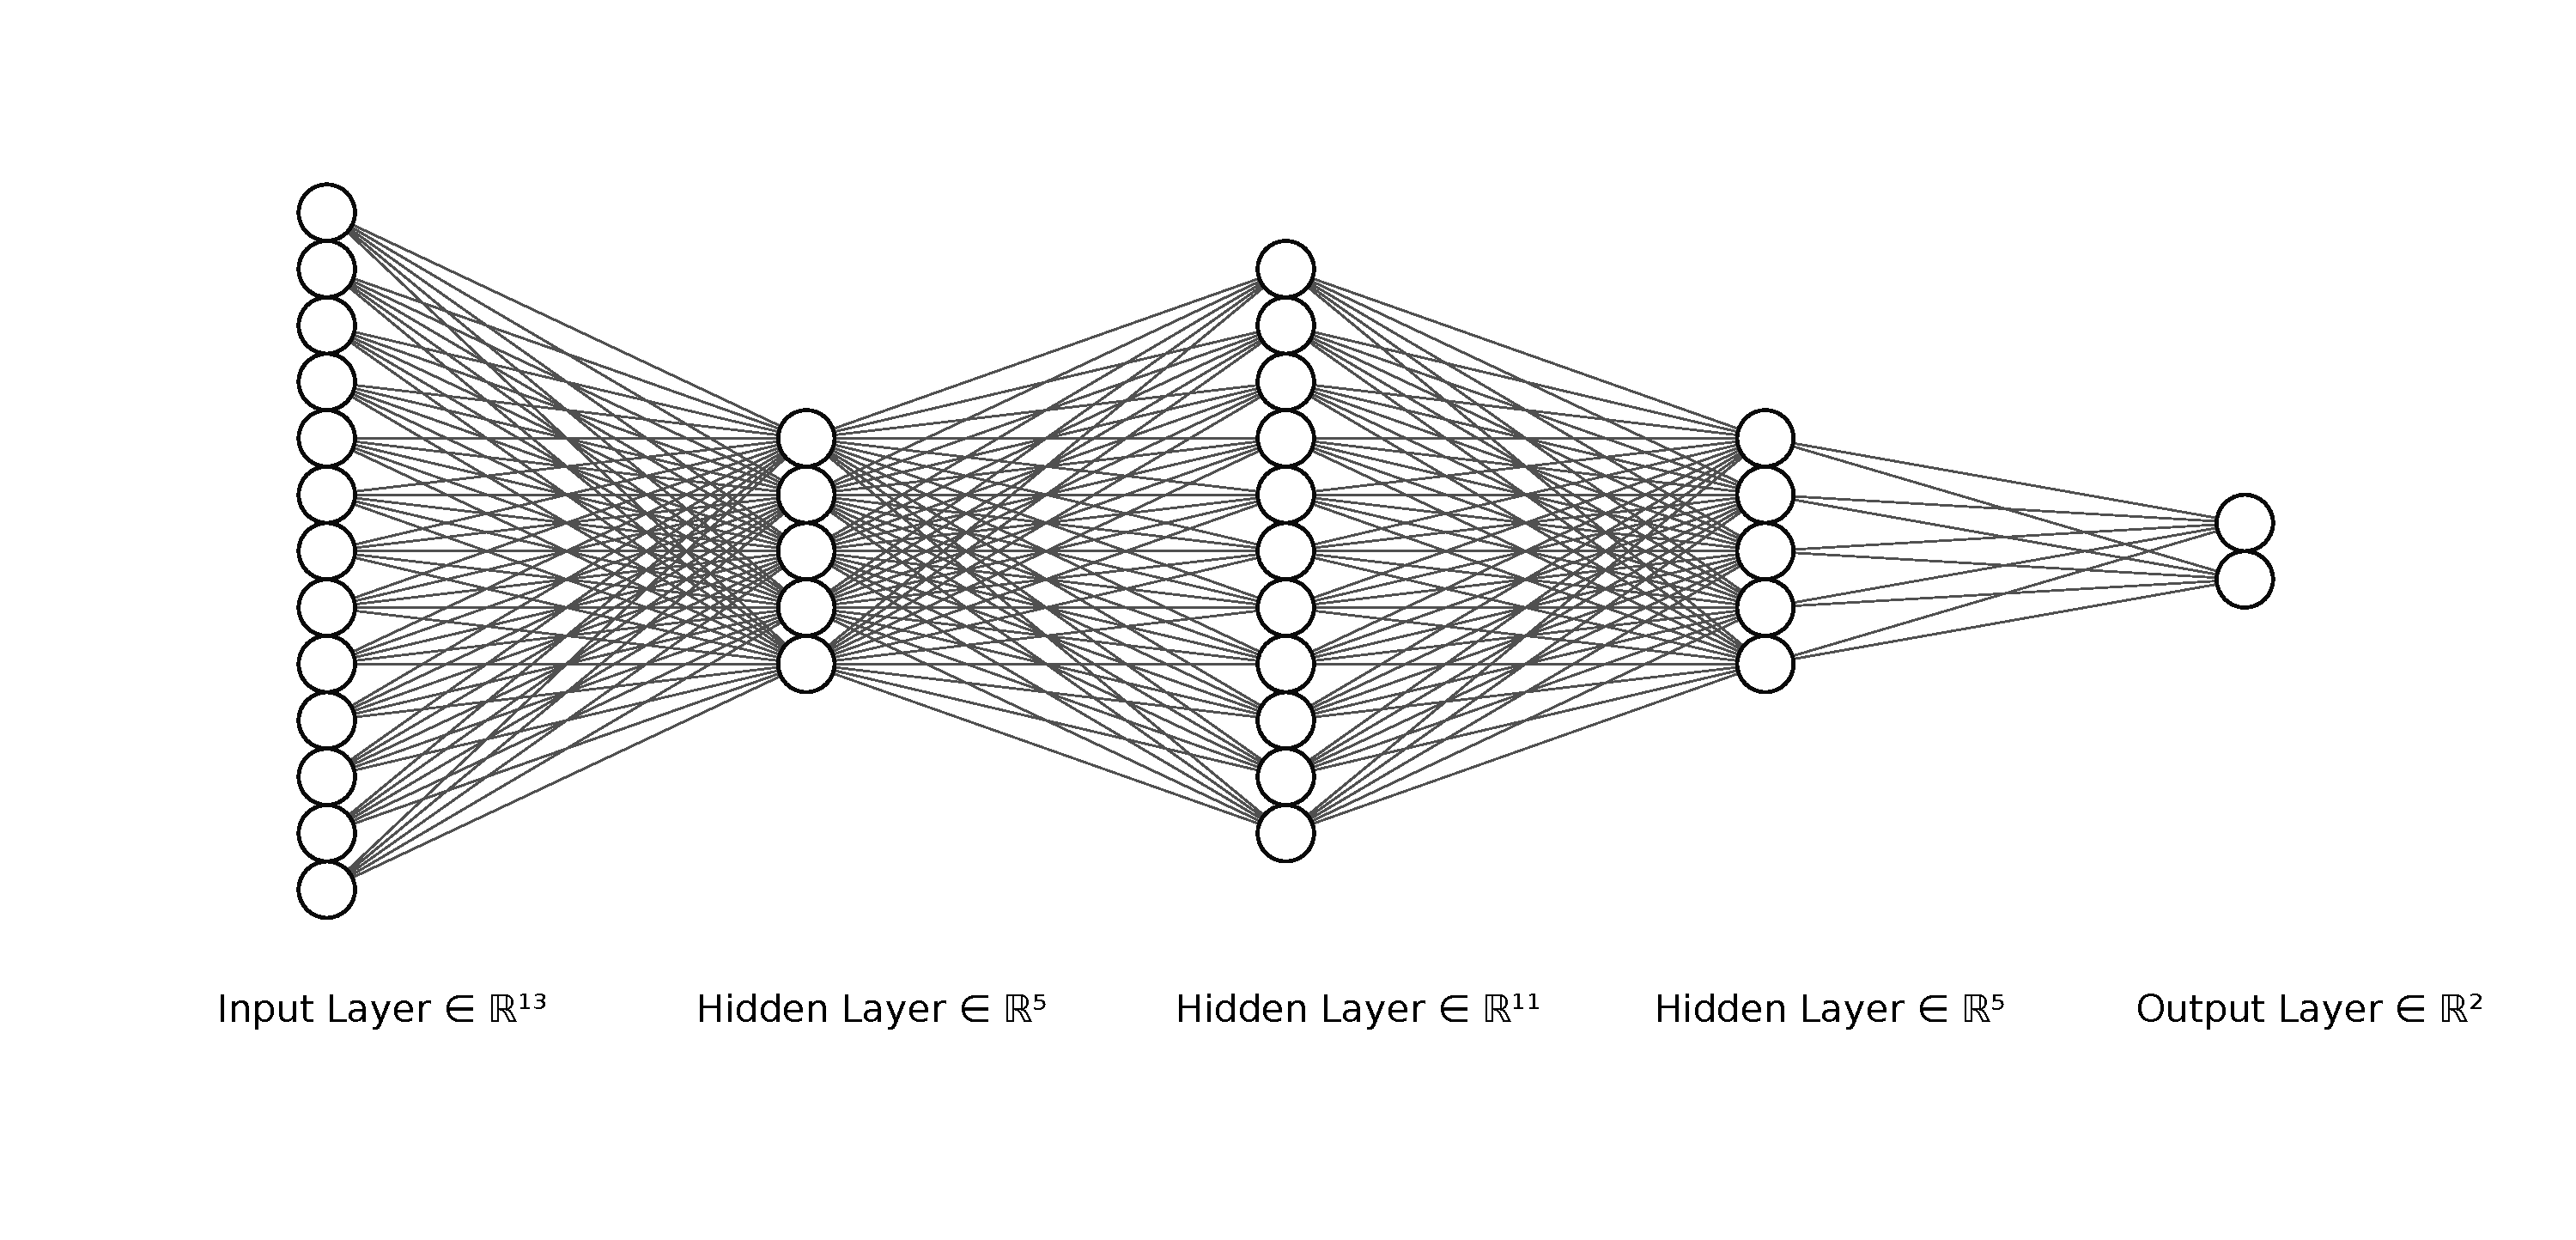
\includegraphics[width=16.0cm, trim={4cm 4.0cm 0.5cm 3.5cm},clip]{plots/Images/nn.pdf}
	\caption{NN example for $z=5$, where input and output layer are only illustrative.}
	\label{NN}
\end{figure}

\begin{para}{Model Complexity}As was mentioned in section \ref{MILtraining}, defining such model for the MIL problem is very complex task, therefore choosing a right model complexity metric is not trivial. Consider a neural network consisting of input layer, 3 hidden layers $h_1\in \R^z, h_2\in \R^{2z+1}, h_3\in \R^z$ and output layer. Then $z \in \left\{1,2,3\dots,20 \right\}$ was selected as model complexity metrics, because this is one of the easiest ways, how to control complexity of the defined MIL model. To gain a better insight, example of such NN is illustrated in Figure \ref{NN}, however this is not the exact NN used in HMill.
\end{para}     

\begin{para}{Prediction Error}
For prediction error metrics will be simply used standard cross--entropy loss  as outlined at the beginning of this section.  There is no need for any trickier objective. Let the total cross--entropy loss evaluated on $k^{\mathrm{th}}$ random split for fixed $z$ be denoted by $\pazocal{L}_k(z)$, then the estimated prediction error is given by 
\begin{equation}
	\widehat{\mathrm{Err}}(z) = \frac{1}{r}\sum_{k=1}^r \pazocal{L}_k(z).
\end{equation}
\end{para}
\vspace{1cm}

To summarize,  we fit 100 models for selected $z$ on train data and evaluate prediction error for all of them on test data, then we take mean value. This process is repeated for each $z~\in~\left\{1,2,3\dots,20 \right\}$, giving 2000 models in total. 
\subsection{Results}
As can be seen in Figure \ref{CV}, obtained results are totally expected. The prediction error evaluated on the training data for higher model complexity approaches zero. However, testing data give oscillating curves with an increasing trend (with a little exception of Musk1), therefore the model selection is necessary. This applies for each dataset.  In addition, following table \ref{tab:resultsCV} numerically summarizes the results evaluated on testing data. 

\begin{figure}[h]
	\centering
	\subfloat[CV for dataset Musk1.]
	{{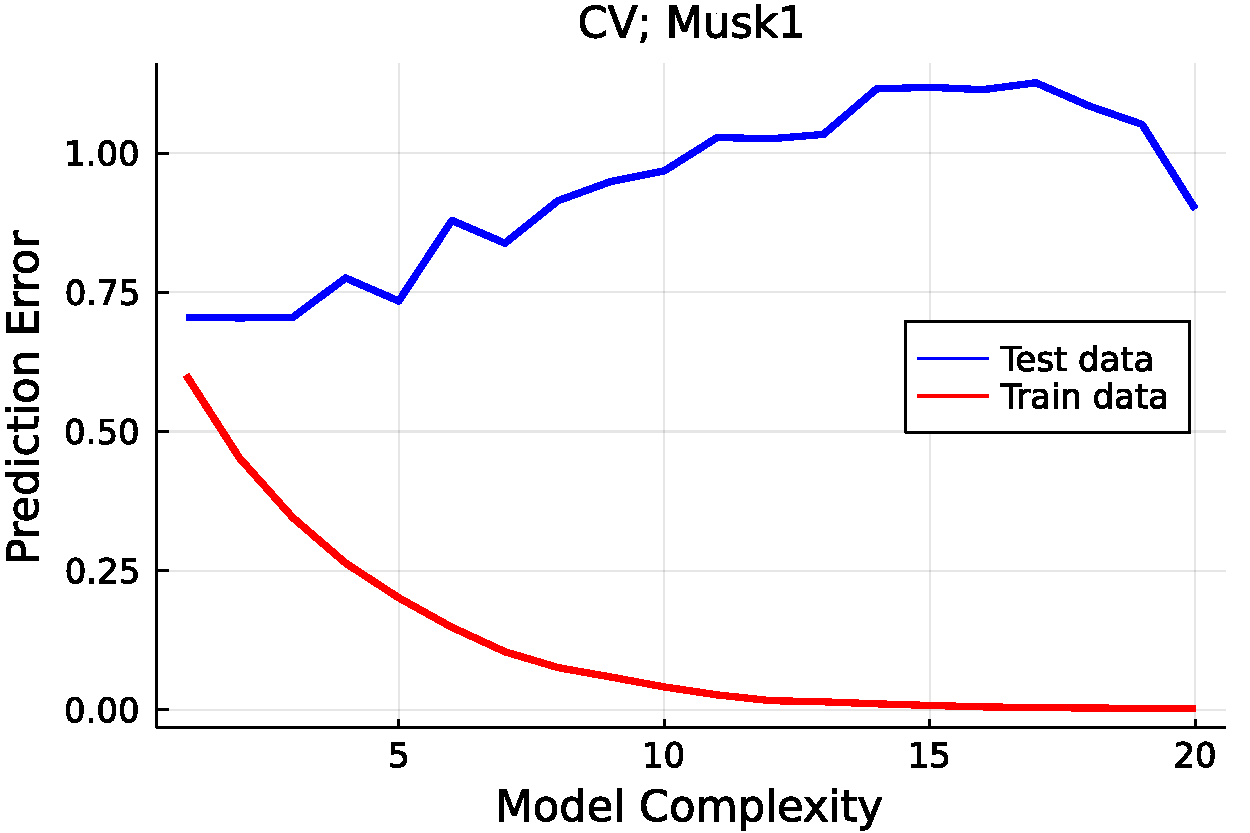
\includegraphics[width=8.0cm]{plots/Images/KFCV_Musk4.pdf} }}%
	\subfloat[CV for dataset Musk2.]
	{{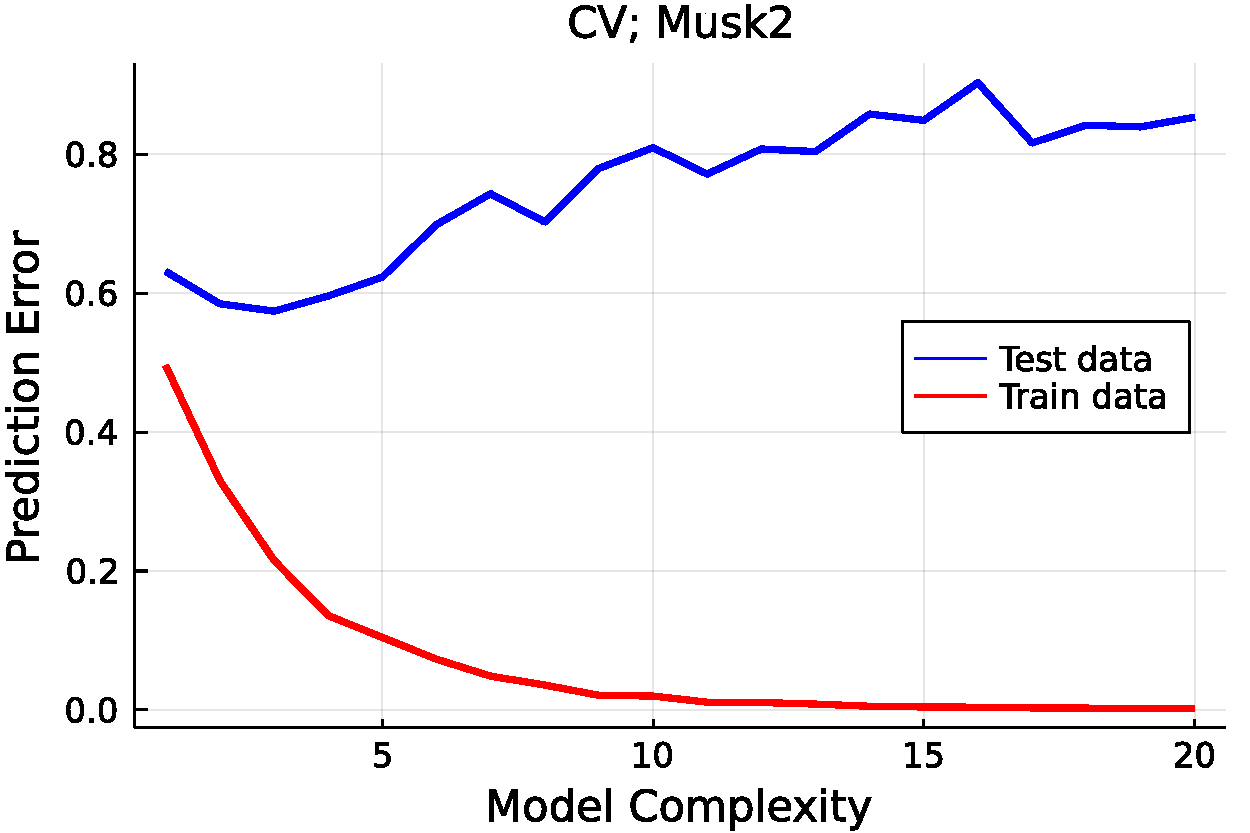
\includegraphics[width=8.0cm]{plots/Images/KFCV_Musk2.pdf} }}%
	\
	\subfloat[CV for dataset Fox.]
	{{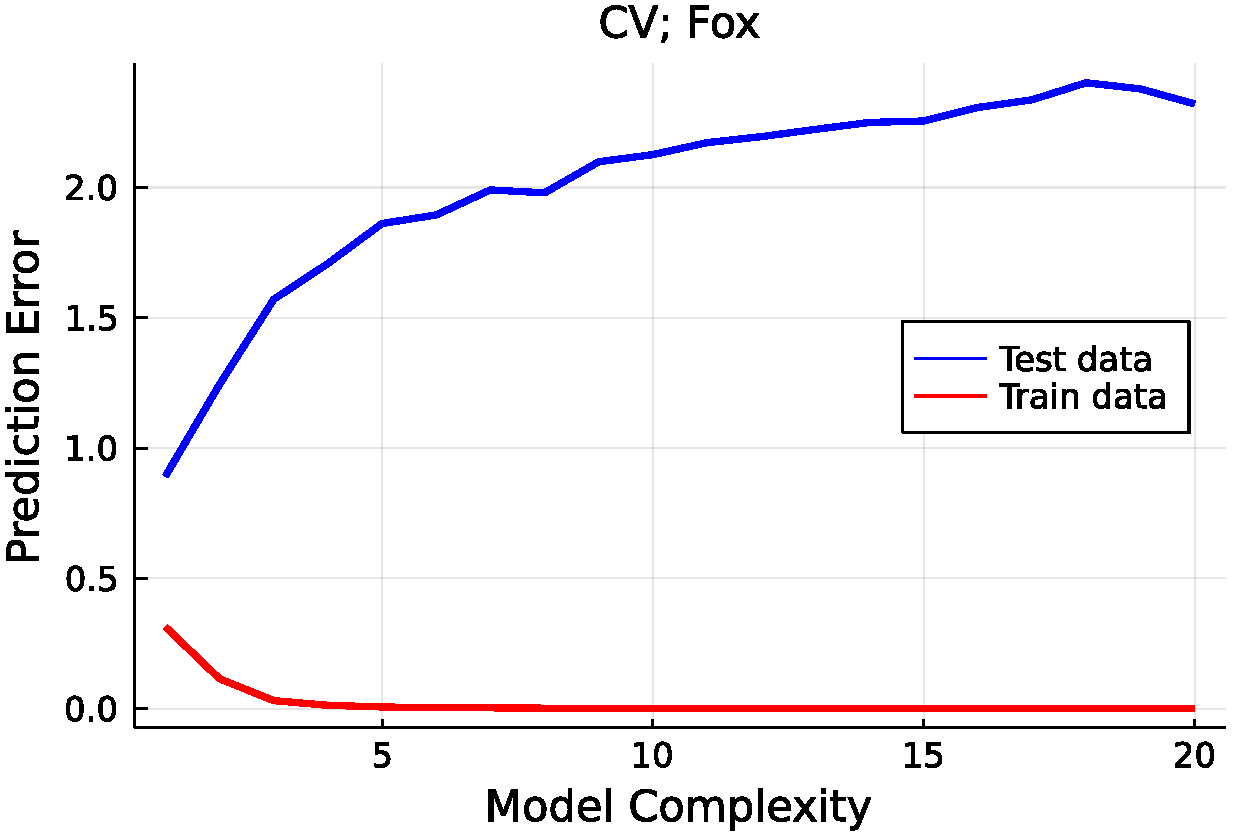
\includegraphics[width=8.0cm]{plots/Images/KFCV_Fox.pdf} }}%
	\subfloat[CV for dataset Tiger.]
	{{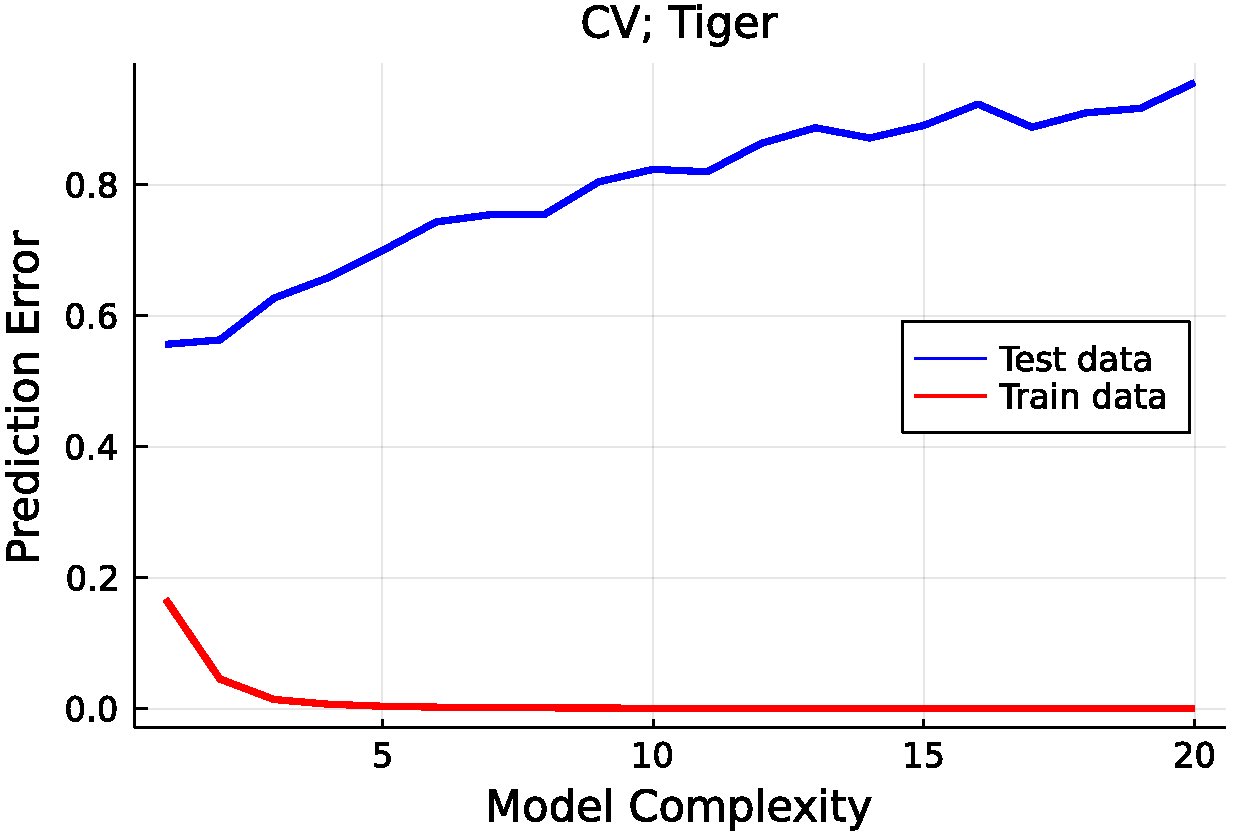
\includegraphics[width=8.0cm]{plots/Images/KFCV_Tiger.pdf} }}%
	\caption{Evaluation of prediction error with the use of training data and testing data on MIL datasets Musk1, Musk2, Fox and Tiger. }%
	\label{CV}%
\end{figure}

\begin{table}[h]
	\centering
	\begin{tabular}{|l|l|l|l|}
		\hline
		Dataset  &$\argmin \widehat{\mathrm{Err}}(z)$ & $ \min \widehat{\mathrm{Err}}(z)$ &$\widehat{\mathrm{Err}}(z=10)$ \\ \hline
		Musk1              & 2        & 0.70& 0.97   \\ \hline
		Musk2              & 3        & 0.57& 0.81   \\ \hline
		Fox               & 1        & 0.89 &  2.13 \\ \hline
		Tiger               & 1        & 0.56  & 0.82    \\ \hline
	\end{tabular}
	\caption{Results of CV evaluated on the testing data.}
	\label{tab:resultsCV}
\end{table}




\section{MIL to HDGM problem}
In the previous part was performed the CV experiment with expected results. However, the estimated prediction error seems to be rather high. Logically, the question has been raised whether the prediction error can be reduced and also whether it is possible to make $r$ smaller.
\subsection{Setup}
On the initiative of reducing the prediction error, it is proposed to train a MIL model that is obtained by minimizing the hybrid loss function 

\begin{equation}
	\min_{\boldsymbol{\theta}}- \mathbb{E}_{p_{\mathrm{data}}(\boldsymbol{x},y)}\left[\alpha\log \frac{\exp\left({f_{\boldsymbol{\theta}}\left(\boldsymbol{x}\right)[y]}\right)}{\sum_{i=1}^C\exp\left({f_{\boldsymbol{\theta}}\left(\boldsymbol{x}\right)[y_i]}\right)}+ \left(1-\alpha\right)\log \frac{\exp\left({f_{\boldsymbol{\theta}}\left(\boldsymbol{x}_i\right)[y]}\right)}{\sum_{j=1}^N\exp\left({f_{\boldsymbol{\theta}}\left(\boldsymbol{x}_j\right)[y]}\right)} \right].
	\end{equation}
Since the discriminative part is already used in HMill framework, the only task is to add the generative part into it. At this point are available all normalization samples, thus $M=N$. This modification should lead to a reduced prediction error evaluated on training data.\\
In the first part of this experiment, we would like to train models in relation to parameter $\alpha$. For this setup, we need to choose fixed $z$. Since authors of \cite{mandlik} usually use $z=10$, we use this value as well. For the prediction error evaluation is used standard cross--entropy as in the previous experiment, again with $r=100$ and $\alpha \in \left\{0.0, 0.1, 0.2,\dots,1.0\right\}$. Therefore estimated prediction error can be written in the form
\begin{equation}
	\widehat{\mathrm{Err}}(\alpha) = \frac{1}{r}\sum_{k=1}^r \pazocal{L}_k(z=10, \alpha).
\end{equation}
We hope to see a curve in the shape of a bowl, having its global minimum in a point $\alpha=0.5$ or somewhere near.\\ 
In the second part, evaluating of the prediction error is approached the other way. Fixed $\alpha = 0.5$ is selected and the dependency on $z~\in~\left\{1,2,3\dots,20 \right\}$ is evaluated as in the section \ref{experimentCV}. Finally, estimated prediction error in this case is defined by
\begin{equation}
	\widehat{\mathrm{Err}}(z) = \frac{1}{r}\sum_{k=1}^r \pazocal{L}_k(z, \alpha =0.5).
\end{equation}
In other words, the setup is the same as in the \ref{experimentCV}, therefore obtained results will be added to the Figure \ref{CV} and table \ref{tab:resultsCV} for a convenient comparison. Note that curves for train data from this experiment will be omitted, since they are not important at this point. We are only interested in predictions for test data.  
\clearpage
\subsection{Results}



Results of the first part are represented in Figure \ref{fig:HDGE} and in Table \ref{tab:resultsHDGE}, where can be seen that adding the generative term into the MIL loss function decreased the prediction error evaluated on all datasets. This improvement is considerable on datasets Musk1 and Musk2, where a can be seen a nice bowl. On datasets Fox and Tiger such improvement does not occur. This means that HDGM approach works, thus a regularization in the form of very simple generative term may bring improvement in predictions. Unfortunately, the choice of $\alpha=0.5$ was not confirmed as the best in our experiment, see Table \ref{tab:resultsHDGE}.   \\
In the second part of the experiment results are shown in Figure \ref{fig:resultsHDGMz} and in Table \ref{tab:HDGMz}. Here is the situation very similar to the previous part of this experiment. Improvement of the prediction error is quite noticeable on first two datasets Musk1 and Musk2, while Fox and Tiger does not look so convincingly. In addition, number of random splits $r=100$ is still needed to get rid of the noise on the prediction error. \\
Overall, it can be said that HDGM approach leads to the decreased prediction error in a small way. 
\begin{table}[h]
	\centering
	\begin{tabular}{|l|l|l|l|}
		\hline
		Dataset  &  $\argmin \widehat{\mathrm{Err}}(\alpha)$& $\min \widehat{\mathrm{Err}}(\alpha)$ \\ \hline
		Musk1              & 0.4      & 0.68   \\ \hline
		Musk2             & 0.2      & 0.54   \\ \hline
		Fox                 & 0.7      & 1.89  \\ \hline
		Tiger            & 0.4      & 0.74      \\ \hline
	\end{tabular}
	\caption{Prediction error statistics for HDGM in case of $z=10$.}
	\label{tab:resultsHDGE}
\end{table}
\begin{figure}[h]
	\centering
	\subfloat[HDGM for dataset Musk1.]
	{{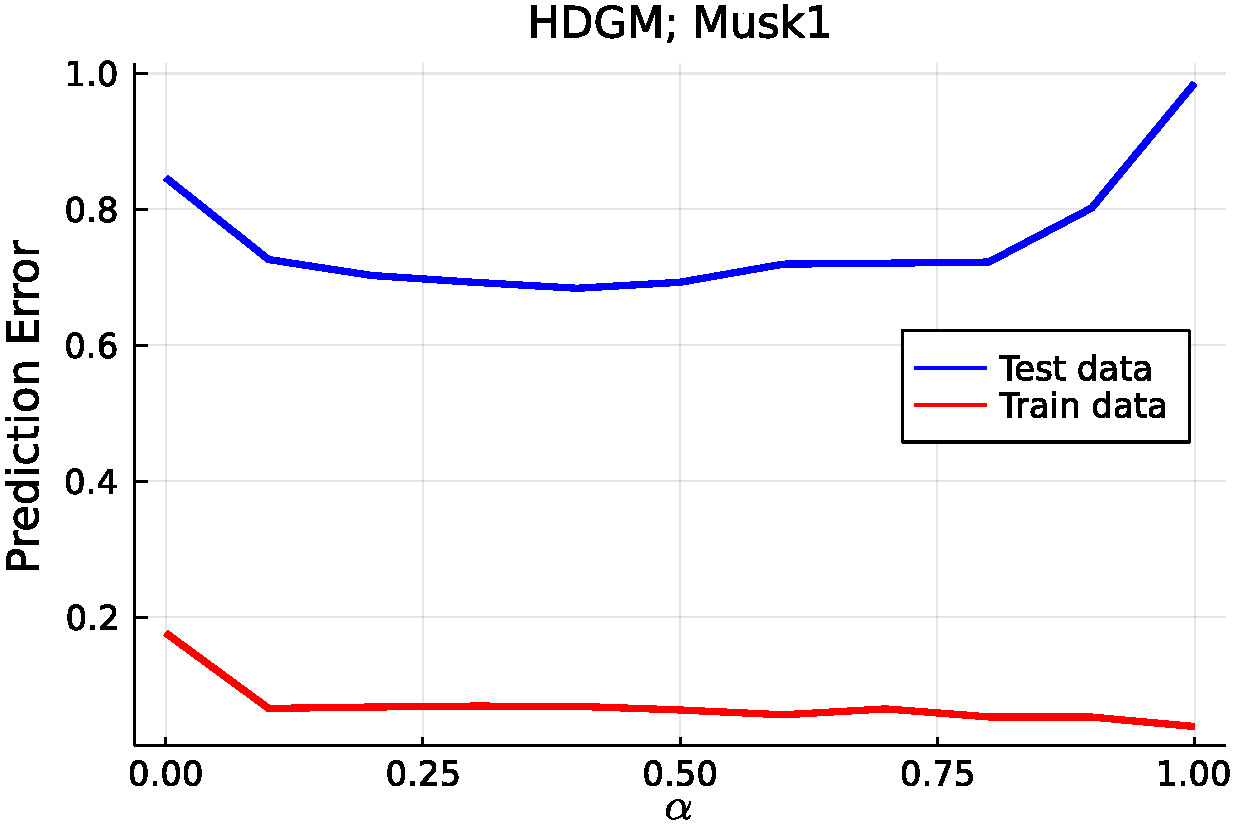
\includegraphics[width=8.2cm]{plots/Images/HDGM_Musk3.pdf} }}%
	\subfloat[HDGM for dataset Musk2.]
	{{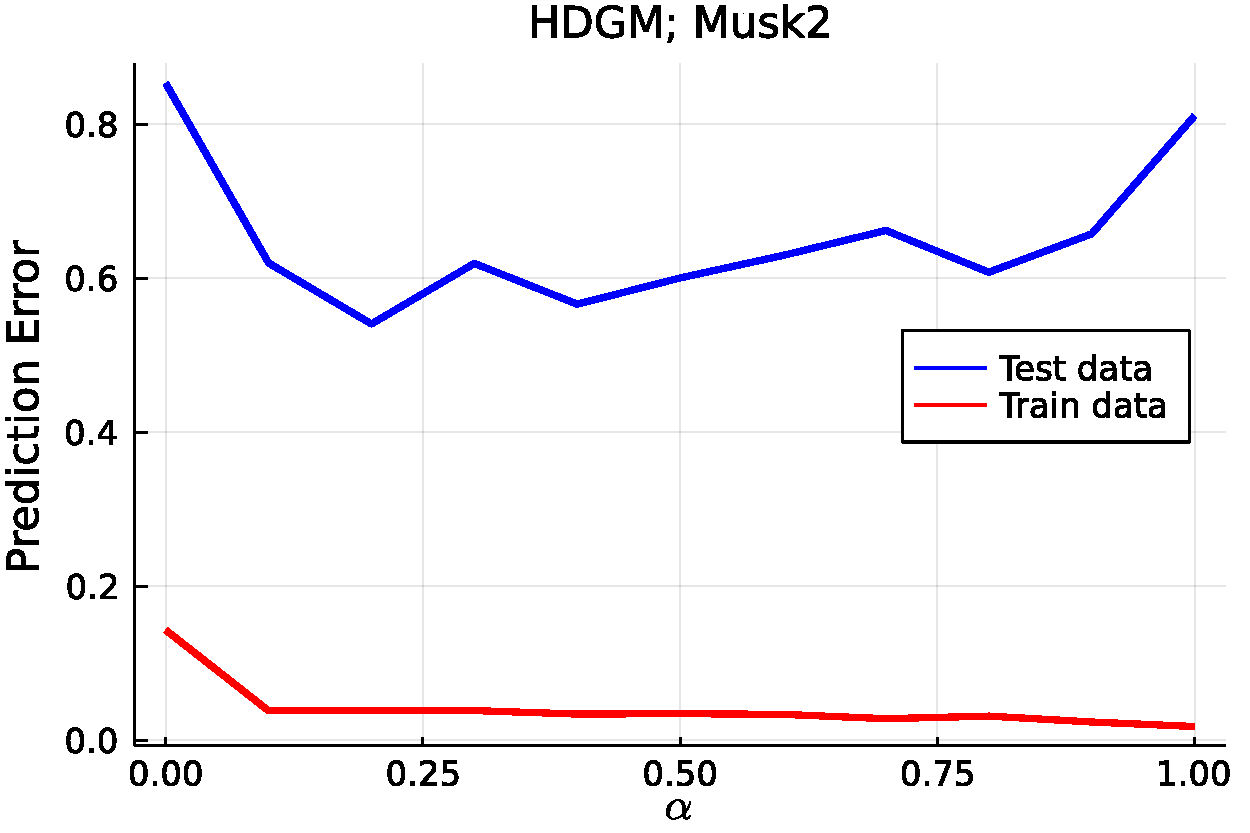
\includegraphics[width=8.2cm]{plots/Images/HDGM_Musk4.pdf} }}%
	\
	\subfloat[HDGM for dataset Fox.]
	{{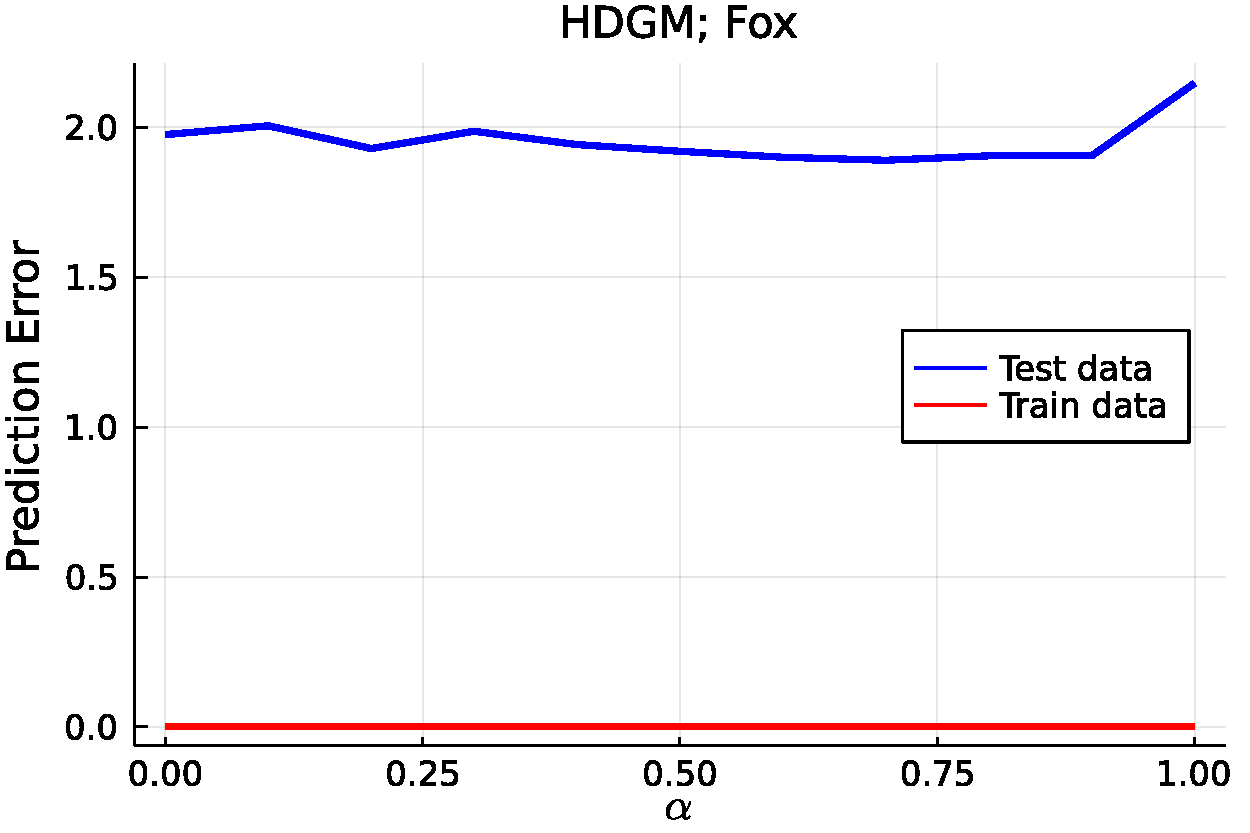
\includegraphics[width=8.2cm]{plots/Images/HDGM_Fox.pdf} }}%
	\subfloat[HDGM for dataset Tiger.]
	{{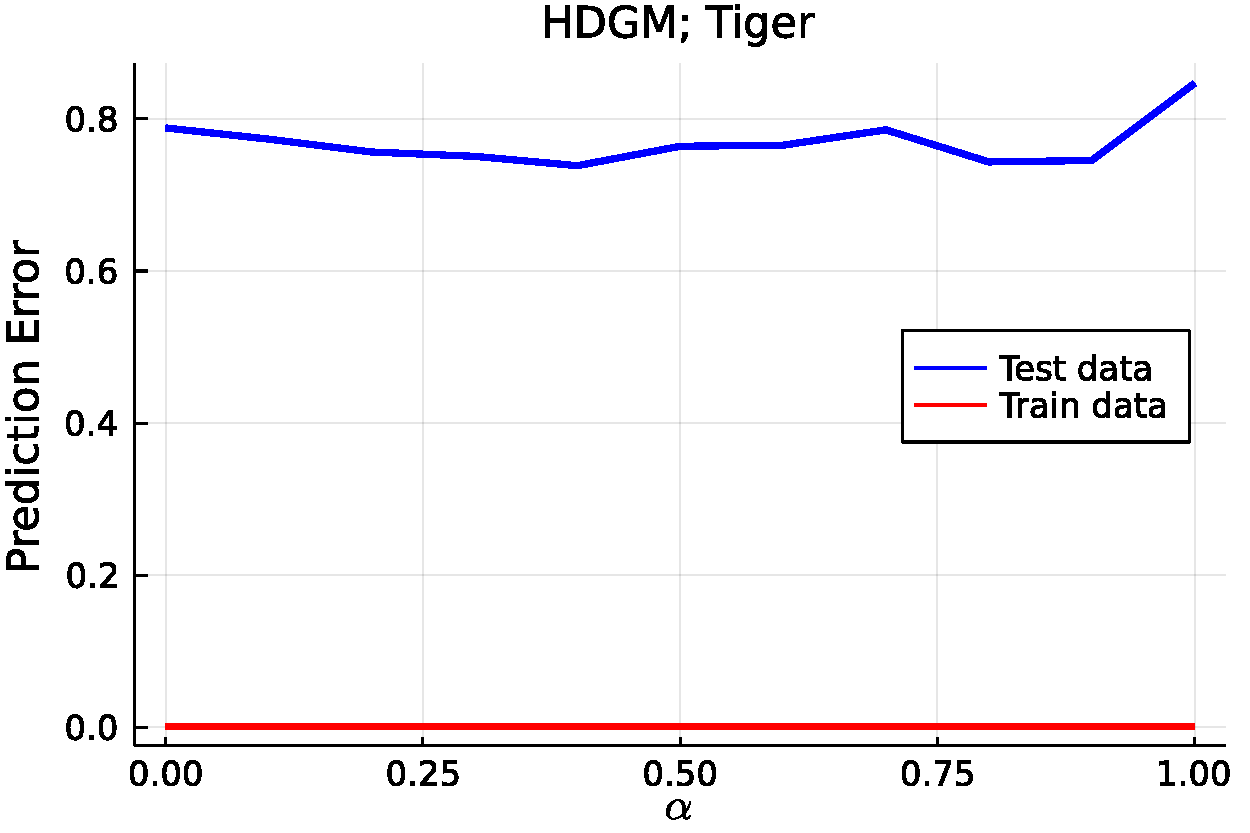
\includegraphics[width=8.2cm]{plots/Images/HDGM_Tiger.pdf} }}
	\caption{Evaluation of the prediction error $\widehat{\mathrm{Err}}(\alpha)$ with the use of training data and testing data on MIL datasets. }%
	\label{fig:HDGE}%
\end{figure}


\begin{table}[h]
	\centering
	\begin{tabular}{|l|l|l|l||l|l|l|}
		\hline
		& \multicolumn{3}{l||}{~~~~~~~~~~~\textbf{Discriminative part only}} & \multicolumn{3}{l|}{~~~~~~~~~~~~~~~~~\textbf{HDGM}; $\alpha=0.5$} \\ \hline
		Dataset & $\argmin \widehat{\mathrm{Err}}(z)$   & $\min \widehat{\mathrm{Err}}(z)$ &$\widehat{\mathrm{Err}}(z=10)$  &   $\argmin \widehat{\mathrm{Err}}(z)$             &     $\min \widehat{\mathrm{Err}}(z)$       &     $\widehat{\mathrm{Err}}(z=10)$         \\ \hline
		Musk1   & 2             & 0.70         & 0.97    &    6          &  0.64           &  \textbf{0.69}           \\ \hline
		Musk2   & 3              & 0.57         & 0.81    &    6          & 0.55            &  \textbf{0.66}           \\ \hline
		Fox     & 1              & 0.89         & 2.13    &    1          &  0.95           &   \textbf{1.96}          \\ \hline
		Tiger   & 1              & 0.56          & 0.82       &   2           &   0.58          &   \textbf{0.80}          \\ \hline
	\end{tabular}
	\caption{Comparison of prediction error statistics for HDGM $\alpha=0.5$ and discriminative part only. Pay attention especially to the last column in each approach, $\widehat{\mathrm{Err}}(z=10)$.}
	\label{tab:HDGMz}
\end{table}

\begin{figure}[h]
	\centering
	\subfloat[HDGM: $\alpha=0.5$ vs Discriminative; Musk1.]
	{{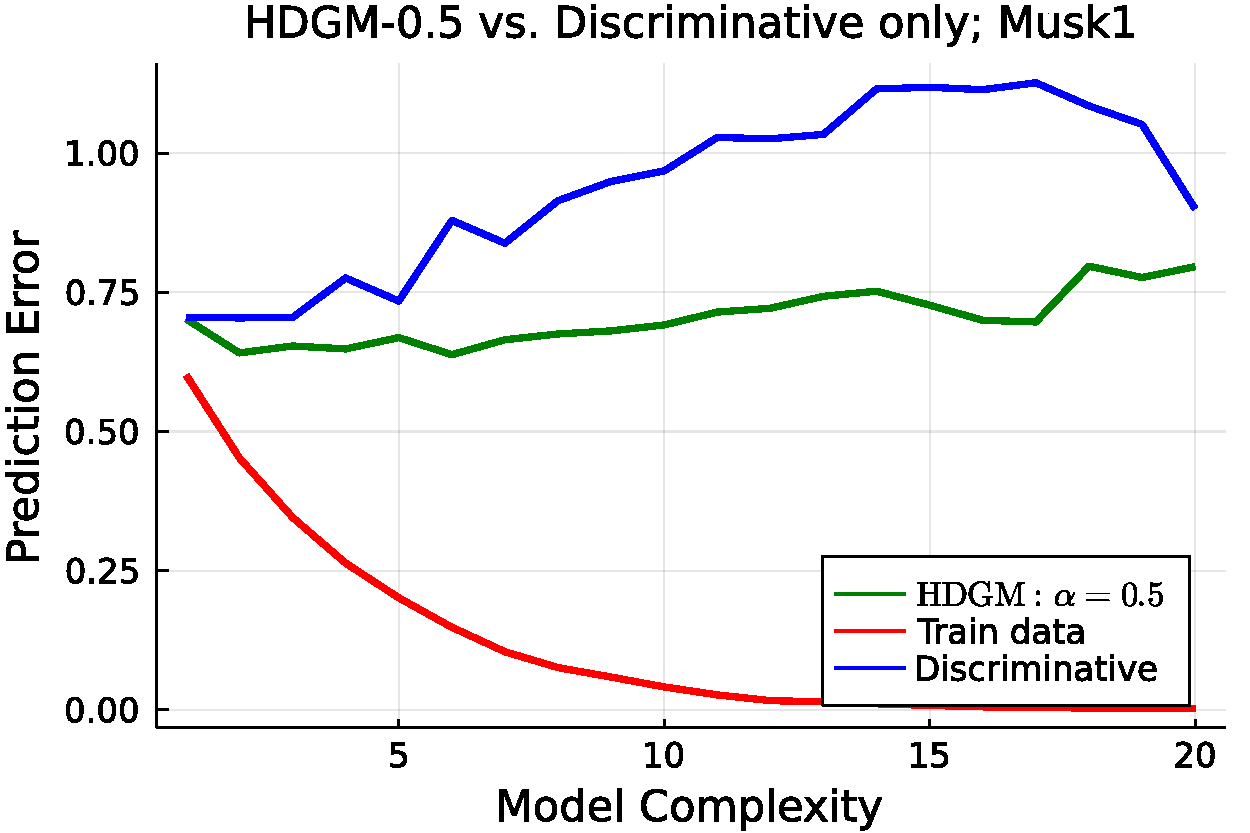
\includegraphics[width=8.2cm]{plots/Images/supervisedvsHDGM0_5_Musk1.pdf} }}%
	\subfloat[HDGM: $\alpha=0.5$ vs Discriminative; Musk2.]
	{{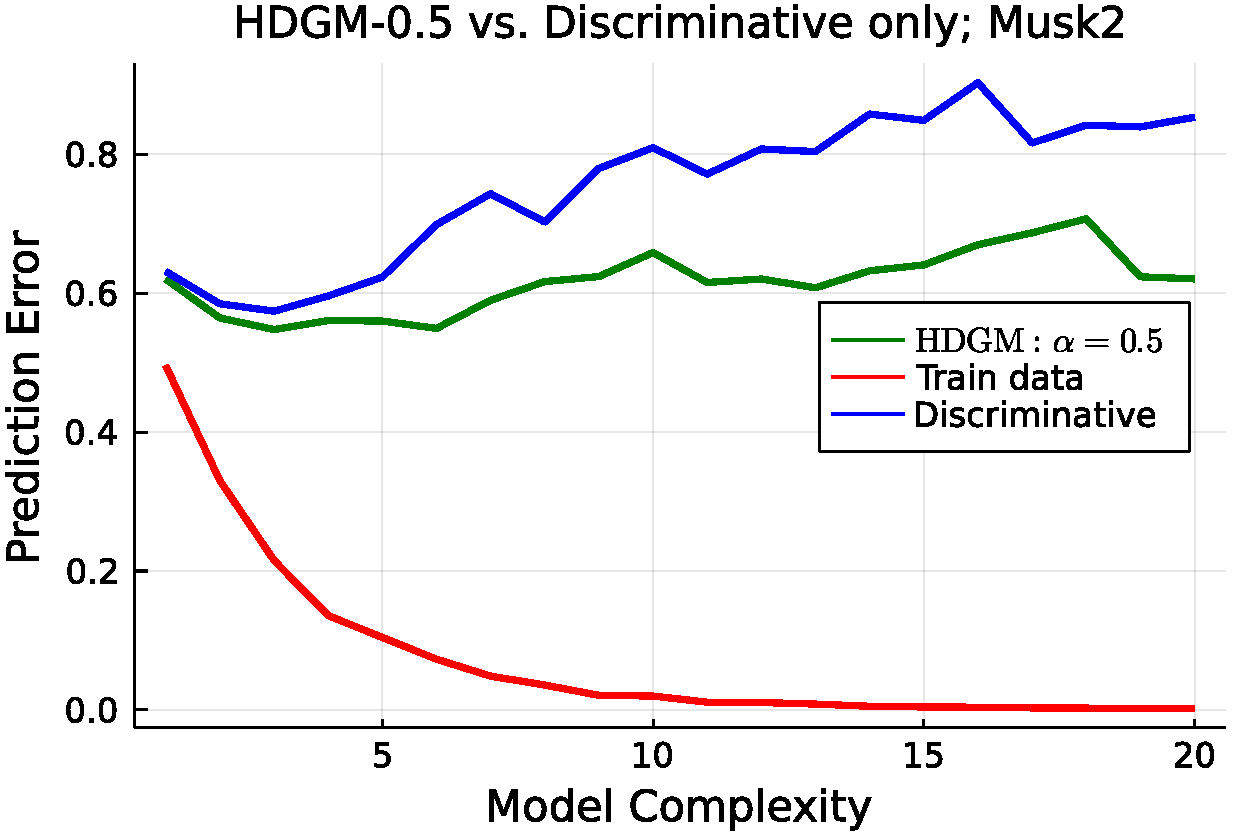
\includegraphics[width=8.2cm]{plots/Images/supervisedvsHDGM0_5_Musk2.pdf} }}%
	\
	\subfloat[HDGM: $\alpha=0.5$ vs Discriminative; Fox.]
	{{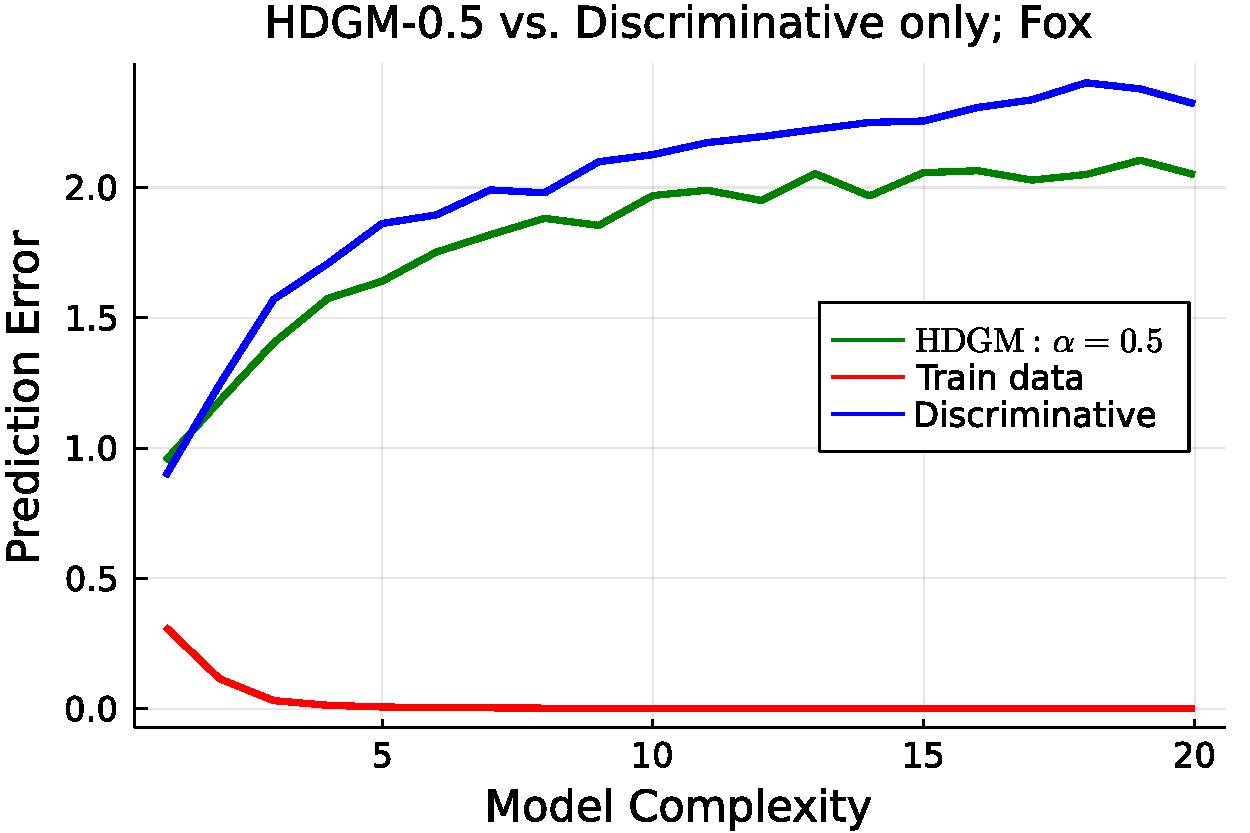
\includegraphics[width=8.2cm]{plots/Images/supervisedvsHDGM0_5_Fox.pdf} }}%
	\subfloat[HDGM: $\alpha=0.5$ vs Discriminative; Tiger.]
	{{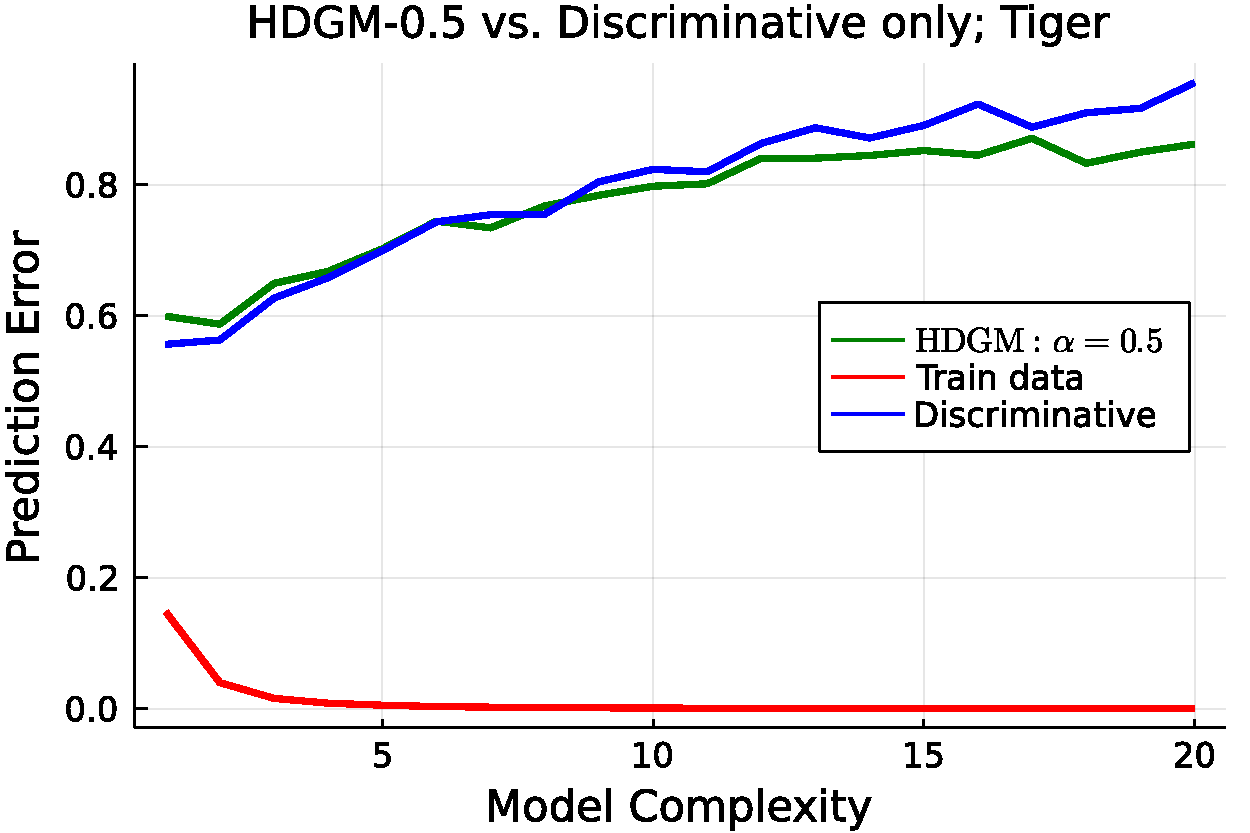
\includegraphics[width=8.2cm]{plots/Images/supervisedvsHDGM0_5_Tiger.pdf} }}
\caption{Comparison of the prediction error  $\widehat{\mathrm{Err}}(z)$ for HDGM $\alpha=0.5$ and discriminative part only. }%
	\label{fig:resultsHDGMz}%
\end{figure}


\chapter*{Conclusion}

\pagestyle{plain}

\addcontentsline{toc}{chapter}{Conclusion}
At the beginning of this work, supervised learning and energy-based models were introduced. The following passage consists of contrastive learning, which was briefly reviewed, and thereafter supervised learning and contrastive learning was merged into hybrid discriminative and generative models. Subsequently, this approach was applied and tested on a simple example consisting of polynomial regression.
After this example, we briefly introduce multiple instance learning with a short description of the embedded space and its way of training. As a first MIL experiment, cross--validation was performed on four MIL datasets, where enough space was given to a proper definition of the model complexity metrics.  The results obtained were completely expected; they included decreasing prediction errors for train data and increasing for test data. In the next step, a solution was searched on how to decrease the prediction error evaluated on the test data. In this initiative, HDGM was trained instead of a standard discriminative model. In the consecutive result, HDGM was found to lead to a decrease in prediction error, however, nothing significant. In addition, a large number of random splits of the data set were still necessary to eliminate the noise from the prediction error.
In conclusion, this approach has proven to be functional, although a proposed generative regularization is very simple and can be replaced by much more complicated models. From this point of view, this approach has great potential that has not yet been fully exploited.


\begin{thebibliography}{1}

\bibitem{bishop}Christopher M.Bishop: \emph{Pattern recognition and machine learning}. [New York]: Springer, 2006. Information science and statistics. ISBN 0-387-31073-8.

\bibitem{mandlik}S.Mandlik.: \emph{Mapping the Internet: Modelling Entity
	Interactions in Complex Heterogeneous Networks}. arXiv preprint arXiv:2104.09650.

\bibitem{Pevnak}T. Pevny and P. Somol: 	\emph{Discriminative models for multi-instance problems with tree structure.} In Proceedings of the 2016 ACM Workshop on Artificial Intelligence and Security, 2016, 83-91.

\bibitem{MIL}J. Wu, S. Pan, X. Zhu, C. Zhang, X. Wu: \emph{Multi-instance learning with discriminative bag mapping.} IEEE Transactions on Knowledge and Data Engineering, 30(6), 2018, 1065-1080.

\bibitem{jeffrey}H. Jeffrey: \emph{An invariant form for the prior probability in estimation problems.} Proceedings of the Royal Society of London. Series A. Mathematical and Physical Sciences. 1946, 1--9.

\bibitem{generativevsdisriminative} M. I. Jordan and A. Y. Ng. :\emph{On discriminative vs. generative classifiers: A comparison of logistic regression and naive bayes.} Advances in neural information processing systems.  2002.

\bibitem{KL}D. Commenges: \emph{Information Theory and Statistics: an overview.} ArXiv preprint arXiv:1511.00860, 2015,  1--22.

\bibitem{Bigp}J. Brownlee: \emph{How to Handle Big-p, Little-n (p >> n) in Machine Learning}. (2020). [on-line]. Available from: \url{https://machinelearningmastery.com/how-to-handle-big-p-little-n-p-n-in-machine-learning/}.

\bibitem{smidl} V. Smidl: \emph{The Variational Bayes Approach in Signal procesing}. PhD Thesis. Trinity College Dublin. 2004.

\bibitem{contrastive1} M. Zhuang and M. Collins: \emph{Ma, Zhuang, and Michael Collins. "Noise contrastive estimation and negative sampling for conditional models: Consistency and statistical efficiency.} arXiv preprint arXiv:1809.01812, 2018.

\bibitem{contrastive2} M. Gutmann and A. Hyvärinen: \emph{Noise-contrastive estimation: A new estimation principle for unnormalized statistical models.}  Proceedings of the thirteenth international conference on artificial intelligence and statistics. JMLR Workshop and Conference Proceedings, 2010.

\bibitem{HDGEmain} H. Liu and P. Abbeel: \emph{Hybrid discriminative-generative training via contrastive learning.} arXiv preprint arXiv:2007.09070, 2020.

\bibitem{EM} S.K. Ng, T. Krishnan and G.J.McLachlan: \emph{Handbook of computional statistics}. The EM algorithm. Springer, Berlin, Heidelberg. 2012, 139-172.

\bibitem{energy} W. Gratwohl, K.C. Wang and J.H. Jacobsen: \emph{Your classifier is secretly an energy based model and you should treat it like one.} GRATHWOHL, Will, et al. Your classifier is secretly an energy based model and you should treat it like one. arXiv preprint arXiv:1912.03263, 2019.

\bibitem{energy2} Y. LeCun, S. Chopra, R.Hadsell, M. Ranzato and F. Huang: \emph{A tutorial on energy-based learning.}  Predicting structured data, 2006, 1.0.

\bibitem{MILfirstly} T.G. Dietterich, R.H. Lathrop and T. Lozano-Pérez: \emph{Solving the multiple instance problem with axis-parallel rectangles.}  Artificial intelligence, 1997, 89.1-2: 31-71.

\bibitem{statistics} J. Friedman, T. Hastie and R. Tibshirani: \emph{The elements of statistical learning.} [New York]: Springer, 2001. Series in statistics.

\bibitem{supervised} M. Talabis, R. McPherson, I. Miyamoto, J. Martin and D.Kaye: \emph{Information Security Analytics.} Syngress, 2015.

\bibitem{Julia} J.Bezanson, S. Karpinski, V.B. Skah:\emph{A fast dynamic language for technical computing.} arXiv preprint arXiv:1209.5145, 2012.

\bibitem{speech} D. Yu and L. Deng: \emph{Automatic Speech Recognition.} Springer london limited, 2016.
\end{thebibliography}

\appendix
\chapter{Computional formulas}

\section{Solution of $\KL{\pazocal{N}\left(\boldsymbol{z}; \boldsymbol{\mu},\sigma^2\mathbb{I}_P  \right) }{\pazocal{N}\left(\boldsymbol{z}; \boldsymbol{0},\mathbb{I}_P^{}  \right)}$}
In the VAE section, the ELBO \eqref{eq:VAEloss} is derived and subsequently optimized. One of the ELBO expressions is the KL distance mentioned above. For two multivariate Gaussian distributions we have a KL distance analytical solution. The complete calculation is given here. First, recall that PDF for a multivariate Gaussian distribution in $\R^P$ with mean $\boldsymbol{\mu}$ and covariance matrix $\boldsymbol{\Sigma}$ is defined as
\begin{equation}
    \pazocal{N}\left(\boldsymbol{z}; \boldsymbol{\mu},\boldsymbol{\Sigma}  \right) = \frac{1}{\sqrt{\left(2\pi\right)^P\det\boldsymbol{\Sigma}}}\exp\left(-\frac{1}{2}\left(\boldsymbol{z} - \boldsymbol{\mu}\right)^\top\boldsymbol{\Sigma}^{-1}\left(\boldsymbol{z} - \boldsymbol{\mu}\right) \right).
\end{equation}


\begin{align}
    \mathrm{KL} &= \KL{\pazocal{N}\left(\boldsymbol{z}; \boldsymbol{\mu}_1,\boldsymbol{\Sigma}_1  \right)}{\pazocal{N}\left(\boldsymbol{z}; \boldsymbol{\mu}_2,\boldsymbol{\Sigma}_2  \right)}  = \mathbb{E}_{\pazocal{N}\left(\boldsymbol{\mu}_1,\boldsymbol{\Sigma}_1\right)}\left[\log\pazocal{N}\left(\boldsymbol{\mu}_1,\boldsymbol{\Sigma}_1\right) - \log\pazocal{N}\left(\boldsymbol{\mu}_2,\boldsymbol{\Sigma}_2\right) \right]  
    \\
    &= \frac{1}{2}\mathbb{E}_{\pazocal{N}\left(\boldsymbol{\mu}_1,\boldsymbol{\Sigma}_1\right)}\left[-\log\det\boldsymbol{\Sigma}_1 - \left(\boldsymbol{z} - \boldsymbol{\mu}_1\right)^\top\boldsymbol{\Sigma}^{-1}_1\left(\boldsymbol{z}-\boldsymbol{\mu}_1\right) + \log\det\boldsymbol{\Sigma}_2+\left(\boldsymbol{z} - \boldsymbol{\mu}_1\right)^\top\boldsymbol{\Sigma}^{-1}_1\left(\boldsymbol{z}-\boldsymbol{\mu}_1\right) \right] \\
    &= \frac{1}{2}\log\frac{\det\boldsymbol{\Sigma}_2}{\det\boldsymbol{\Sigma}_1} + \frac{1}{2}\mathbb{E}_{\pazocal{N}\left(\boldsymbol{\mu}_1,\boldsymbol{\Sigma}_1\right)} \left[-\left(\boldsymbol{z} - \boldsymbol{\mu}_1\right)^\top\boldsymbol{\Sigma}^{-1}_1\left(\boldsymbol{z}-\boldsymbol{\mu}_1\right) + \left(\boldsymbol{z} -\boldsymbol{\mu}_2\right)^\top\boldsymbol{\Sigma}^{-1}_2\left(\boldsymbol{z}-\boldsymbol{\mu}_2\right)\right]
    \\
    &= \frac{1}{2}\log\frac{\det\boldsymbol{\Sigma}_2}{\det\boldsymbol{\Sigma}_1} + \frac{1}{2}\mathbb{E}_{\pazocal{N}\left(\boldsymbol{\mu}_1,\boldsymbol{\Sigma}_1\right)} \left[-\Tr\left(\boldsymbol{\Sigma}_1^{-1}\left(\boldsymbol{z} - \boldsymbol{\mu}_1\right)\left(\boldsymbol{z} - \boldsymbol{\mu}_1\right)^\top\right) + \Tr\left(\boldsymbol{\Sigma}_2^{-1}\left(\boldsymbol{z} - \boldsymbol{\mu}_2\right)\left(\boldsymbol{z} - \boldsymbol{\mu}_2\right)^\top\right) \right]
    \\
    &= \frac{1}{2}\log\frac{\det\boldsymbol{\Sigma}_2}{\det\boldsymbol{\Sigma}_1} + \frac{1}{2}\mathbb{E}_{\pazocal{N}\left(\boldsymbol{\mu}_1,\boldsymbol{\Sigma}_1\right)} \left[-\Tr\left(\boldsymbol{\Sigma}_1^{-1}\boldsymbol{\Sigma}_1\right) +  \Tr\left(\boldsymbol{\Sigma}_2^{-1}\left(\bz\bz^\top - 2\bz\boldsymbol{\mu}_2^\top + \boldsymbol{\mu}_2\boldsymbol{\mu}_2^\top \right) \right)\right] 
    \\
    &= \frac{1}{2}\log\frac{\det\boldsymbol{\Sigma}_2}{\det\boldsymbol{\Sigma}_1} - \frac{1}{2}n + \frac{1}{2}\Tr\left(\boldsymbol{\Sigma}_2^{-1}\left(\boldsymbol{\Sigma}_1 +\boldsymbol{\mu}_1\boldsymbol{\mu}_1^\top - 2\boldsymbol{\mu}_2\boldsymbol{\mu}_1^\top  + \boldsymbol{\mu}_2\boldsymbol{\mu}_2^\top \right)\right)
    \\
     &= \frac{1}{2}\left( \log\frac{\det\boldsymbol{\Sigma}_2}{\det\boldsymbol{\Sigma}_1} - n +\Tr\left(\boldsymbol{\Sigma}_2^{-1}\boldsymbol{\Sigma}_1\right) + \Tr\left(\boldsymbol{\mu}_1^\top\boldsymbol{\Sigma}_2^{-1}\boldsymbol{\mu}_1 - 2\boldsymbol{\mu}_1^\top\boldsymbol{\Sigma}_2^{-1}\boldsymbol{\mu}_2 + \boldsymbol{\mu}_2^\top\boldsymbol{\Sigma}_2^{-1}\boldsymbol{\mu}_2 \right)\right)
     \\
      &=\frac{1}{2}\left( \log\frac{\det\boldsymbol{\Sigma}_2}{\det\boldsymbol{\Sigma}_1} - n +\Tr\left(\boldsymbol{\Sigma}_2^{-1}\boldsymbol{\Sigma}_1\right) + \left(\boldsymbol{\mu}_2 - \boldsymbol{\mu}_1\right)^\top\boldsymbol{\Sigma}_2^{-1}\left(\boldsymbol{\mu}_2 - \boldsymbol{\mu}_1\right)\right)
\end{align}
\end{document}
